\chapter[The \index{B^n@\({B}^{n}\)!fundamental group}Fundamental Group]{The Fundamental Group}
\vspace{6.5cm}
\chaptermark{The Fundamental Group}


One of the basic problems of topology is to determine whether two given topological spaces are homeomorphic or not. There is no method for solving this problem in general, but techniques do exist that apply in particular cases.

Showing that two spaces are homeomorphic is a matter of constructing a continuous mapping from one to the other having a continuous inverse, and constructing continuous functions is a problem that we have developed techniques to handle.

Showing that two spaces are not homeomorphic is a different matter. For that, one must show that a continuous function with continuous inverse does not exist. If one can find some topological property that holds for one space but not for the other, then the problem is solved一the spaces cannot be homeomorphic. The closed interval \([  {0,1}]\) cannot be homeomorphic to the open interval(0,1), for instance, because the \index{first homotopy group (see fundamental group)@First homotopy group (see Fundamental group)} first space is compact and the second one is not. And the real line \(\mathbb{R}\) cannot be homeomorphic to the ``long line'' \(L\) , because \(\mathbb{R}\) has a countable basis and \(L\) does not. Nor can the real line \(\mathbb{R}\) be homeomorphic to the plane \({\mathbb{R}}^{2}\) ; deleting a point from \({\mathbb{R}}^{2}\) leaves a connected space remaining, and deleting a point from \(\mathbb{R}\) does not.

But the \index{Covering space!topological properties}\index{Covering space!topological properties}\index{Covering space!topological properties}topological properties we have studied up to now do not carry us very far in solving the problem. For instance, how does one show that the plane \({\mathbb{R}}^{2}\) is not homeomorphic to three-dimensional space \({\mathbb{R}}^{3}\) ? As one goes down the list of topological properties—compactness, connectedness, local connectedness, metrizability, and so on-one can find no topological property that d\index{\({P}^{2}\)!is surface}istinguishes between them. As another example, consider such surfaces as the 2-sphere \({S}^{2}\) , the \index{Torus} \(T\) (surface \index{Covering space!of torus}of a doughnut), and the double \index{torus@Torus}\index{torus@Torus}\index{torus@Torus}torus \(T\# T\) (surface of a two-holed doughnut). None of the topological properties we have studied up to now will distinguish between them.

So we must introduce new properties and new techniques. One \index{Fundamental group!of \({S}^{n}\)}of the most natural such properties is that of \index{\({S}^{n}\) (unit sphere)!simple connectedness}\index{\({S}^{n}\) (unit sphere)!simple connectedness}\index{\({S}^{n}\) (unit sphere)!simple connectedness}simple connectedness. You probably have studied this notion already, when you studied line integrals in the plane. Roughly speaking, one says that a space \(X\) is \index{Simply connected} if every closed curve in \(X\) can be shrunk to a point in \(X\) . (We shall make this more precise later.) The property of simple connectedness, it turns out, will distinguish between \({\mathbb{R}}^{2}\) and \({\mathbb{R}}^{3}\) , deleting a point from \({\mathbb{R}}^{3}\) leaves a \index{simply connected@Simply connected}\index{simply connected@Simply connected}\index{simply connected@Simply connected}simply connected space remaining, but deleting a point from \({\mathbb{R}}^{2}\) does not. It will also distinguish between \({S}^{2}\) (which is simply connected) and the torus \(T\) (which is not). But it will not distinguish between \(T\) and \(T\# T\) ; neither of them is simply connected.

There is an idea more general than the idea of simple connectedness, an idea that includes simple connectedness as a \index{Seifert-van Kampen theorem!special case}\index{Seifert-van Kampen theorem!special case}\index{Seifert-van Kampen theorem!special case}special case. It involves a certain group that is called the \index{Fundamental group} of the space. Two spaces that are homeomorphic have \index{\({B}^{n}\)!fundamental group}\index{\({B}^{n}\)!fundamental group}fundamental groups that are isomorphic. And the condition of simple connectedness is just the condition that the \index{Deformation retract!fundamental group of}\index{Deformation retract!fundamental group of}\index{Deformation retract!fundamental group of}fundamental group of \(X\) is the trivial (one-element) group. Thus, the proof that \({S}^{2}\) and \(T\) are not homeomorphic can be rephrased by saying that the fundamental group of \({S}^{2}\) is trivial and the fundamental group of \(T\) is not. The fundamental group will distinguish between more spaces than the condition of simple connectedness will. It can be used, for example, to show that \(T\) and \(T\# T\) are not homeomorphic; it turns out that \(T\) has an abelian fundamental group and \(T\# T\) does not.

In this chapter, we define the fundamental group and study its properties. Then we apply it to a number of problems, including the problem of showing that various spaces, such as those already mentioned, are not homeomorphic.

Other applications include theorems about fixed points and \index{Antipode-preserving} maps of the sphere, as well as the well-known \index{Fundamental theorem of algebra}, which says that every polynomial equation with real or complex coefficients has a root. Finally, there is the famous Jordan curve theorem, which we shall study in the next chapter; it states that every simple closed curve \(C\) in the plane separates the plane into two components, of which \(C\) is the common boundary.

Throughout, we assume familiarity with the \index{quotient group@Quotient group} quotient topology (\$22) and local connectedness (§25).

\section*{§ 51 Homotopy of Paths}

Be\index{Lifting lemma: general!for paths}fore defining the fundamental group \index{Initial point: of an oriented line segment!of a path}of a space \(X\) , we shall consider paths on \(X\) and an equivalence relation called path \index{Homotopy} between them. And we shall define a certain operation on the collection of the equivalence classes that makes it into what is called in algebra a groupoid.

\begin{definition}
	If \(f\) and \({f}^{\prime }\) are continuous maps of the space \(X\) into the space \(Y\) , we say that \(f\) is homotopic to \({f}^{\prime }\) if there is a continuous map \(F : X \times  I \rightarrow  Y\) such that

\[
F( {x,0})  = f( x) \;\text{ and }\;F( {x,1})  = {f}^{\prime }( x)
\]

for each \(x\) . (Here \(I = [  {0,1}]\) .) The map \(F\) is called a \index{homotopy@Homotopy}\index{homotopy@Homotopy}\index{homotopy@Homotopy}homotopy between \(f\) and \({f}^{\prime }\) . If \(f\) is homotopic to \({f}^{\prime }\) , we write \(f \simeq  {f}^{\prime }\) . If \(f \simeq  {f}^{\prime }\) and \({f}^{\prime }\) is a constant map, we say that \(f\) is \index{nulhomotopic map@Nulhomotopic map} nulhomotopic.
\end{definition}

We think of a homotopy as a continuous one-parameter family of maps from \(X\) to \(Y\) If we imagine the parameter \(t\) as representing time, then the homotopy \(F\) represents a continuous ``deforming'' of the map \(f\) to the map \({f}^{\prime }\) , as \(t\) goes from 0 to 1.

Now we consider the special case in which \(f\) is a path in \(X\) . Recall that if \(f\) : \([  {0,1}]   \rightarrow  X\) is a continuous map such that \(f( 0)  = {x}_{0}\) and \(f( 1)  = {x}_{1}\) , we say that \(f\) is a path in \(X\) from \({x}_{0}\) to \({x}_{1}\) . We also say that \({x}_{0}\) is the initial point, and \({x}_{1}\) the final point, of the path \(f\) . In this chapter, we shall for convenience use the interval \(I = [  {0,1}]\) as the domain for all paths.

If \(f\) and \({f}^{\prime }\) are two paths in \(X\) , there is a stronger relation between them than mere homotopy. It is defined as follows:

\begin{definition}
	Two paths \(f\) and \({f}^{\prime }\) , mapping the interval \(I = [  {0,1}]\) into \(X\) , are said to be path homotopic if they have the same initial point \({x}_{0}\) and the same final point \({x}_{1}\) , and if there is a continuous map \(F : I \times  I \rightarrow  X\) such that

\[
F( {s,0})  = f( s) \;\text{ and }\;F( {s,1})  = {f}^{\prime }( s) ,
\]

\[
F( {0,t})  = {x}_{0}\;\text{ and }\;F( {1,t})  = {x}_{1},
\]

for each \(s \in  I\) and each \(t \in  I\) . We call \(F\) a \index{path homotopy@Path homotopy}\index{path homotopy@Path homotopy}\index{path homotopy@Path homotopy}path homotopy between \(f\) and \({f}^{\prime }\) See Figure 51.1. If \(f\) is path homotopic to \({f}^{\prime }\) , we write \(f{ \simeq  }_{p}{f}^{\prime }\) .
\end{definition}

\begin{center}
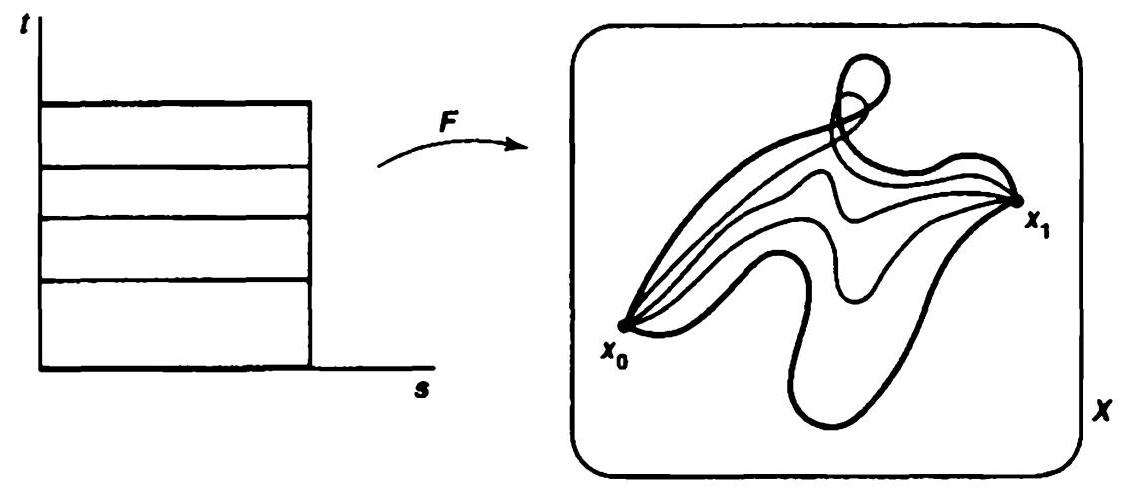
\includegraphics[width=1.0\textwidth]{images/51.1.jpg}
\end{center}
\hspace*{3em} 

Figure 51.1

The first condition says simply that \(F\) is a homotopy between \(f\) and \({f}^{\prime }\) , and the second says that for each \(t\) , the path \({f}_{t}\) defined by the equation \({f}_{t}( s)  = F( {s,t})\) is a path from \({x}_{0}\) to \({x}_{1}\) . Said differently, the first condition says that \(F\) represents a continuous way of deforming the path \(f\) to the path \({f}^{\prime }\) , and the second condition says that the end points of the path remain fixed during the deformation.

\section*{Lemma 51.1. The relations \(\simeq\) and \({ \simeq  }_{p}\) are equivalence relations.}

If \(f\) is a path, we shall denote its path-\index{Homotopy equivalence} class by \([  f]\) .

\begin{proof}
	Let us verify the properties of an equivalence relation.
Given \(f\) , it is trivial that \(f \simeq  f\) ; the map \(F( {x,t})  = f( x)\) is the required homotopy. If \(f\) is a path, \(F\) is a path homotopy.

Given \(f \simeq  {f}^{\prime }\) , we show that \({f}^{\prime } \simeq  f\) . Let \(F\) be a homotopy between \(f\) and \({f}^{\prime }\) . Then \(G( {x,t})  = F( {x,1 - t})\) is a homotopy between \({f}^{\prime }\) and \(f\) . If \(F\) is a path homotopy, so is \(G\) .

Suppose that \(f \simeq  {f}^{\prime }\) and \({f}^{\prime } \simeq  {f}^{\prime \prime }\) . We show that \(f \simeq  {f}^{\prime \prime }\) . Let \(F\) be a homotopy between \(f\) and \({f}^{\prime }\) , and let \({F}^{\prime }\) be a homotopy between \({f}^{\prime }\) and \({f}^{\prime \prime }\) . Define \(G : X \times  I \rightarrow\)  \(\gamma\) by the equation

\[
G( {x,t})  = \{  \begin{array}{ll} F( {x,{2t}}) & \text{ for }t \in  [  {0,\frac{1}{2}}]  , \\  {F}^{\prime }( {x,{2t} - 1}) & \text{ for }t \in  [  {\frac{1}{2},1}]  . \end{array}.
\]

The map \(G\) is well defined, since if \(t = \frac{1}{2}\) , we have \(F( {x,{2t}})  = {f}^{\prime }( x)  = {F}^{\prime }( {x,{2t} - 1})\) . Because \(G\) is continuous on the two closed subsets \(X \times  [  {0,\frac{1}{2}}]\) and \(X \times  [  {\frac{1}{2},1}]\) of \(X \times  I\) , it is continuous on all of \(X \times  I\) , by the pasting lemma. Thus \(G\) is the required homotopy between \(f\) and \({f}^{\prime \prime }\) .

You can check that if \(F\) and \({F}^{\prime }\) are path homotopies, so is \(G\) . See Figure 51.2. is a homotopy between them. It is called a \index{Straight-line homotopy} because it moves the point \(f( x)\) to the point \(g( x)\) along the straight-line segment joining them.

\begin{center}
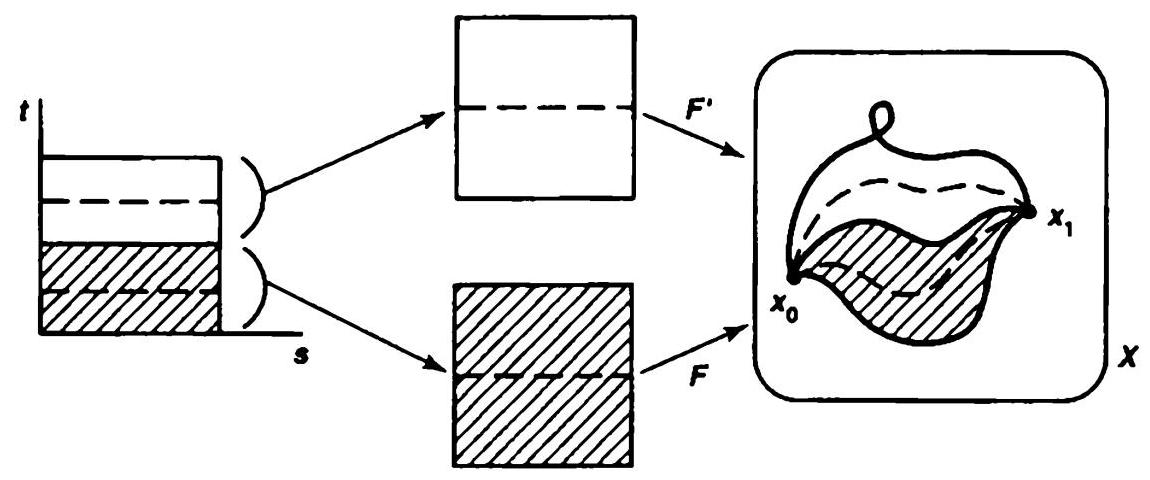
\includegraphics[width=1.0\textwidth]{images/51.2.jpg}
\end{center}
\hspace*{3em} 

Figure 51.2

\begin{centeredblock}
\begin{example}
	Let \(f\) and \(g\) be any two maps of a space \(X\) into \({\mathbb{R}}^{2}\) It is easy to see that \(f\) and \(g\) are homotopic; the map

\[
F( {x,t})  = ( {1 - t}) f( x)  + {tg}( x)
\]

If \(f\) and \(g\) are paths from \({x}_{0}\) to \({x}_{1}\) , then \(F\) will be a path homotopy, as you can check. This situation is pictured in Figure 5.1.3.
\end{example}
\end{centeredblock}

More generally, let \(A\) be any convex subspace of \({\mathbb{R}}^{n}\) . (This means that for any two points \(a,b\) of \(A\) , the straight line segment joining \(a\) and \(b\) is contained in \(A\) .) Then any two paths \(f,g\) in \(A\) from \({x}_{0}\) to \({x}_{1}\) are path homotopic in \(A\) , for the \index{straight-line homotopy@Straight-line homotopy}straight-line homotopy \(F\) between them has image set in \(A\)

\begin{center}
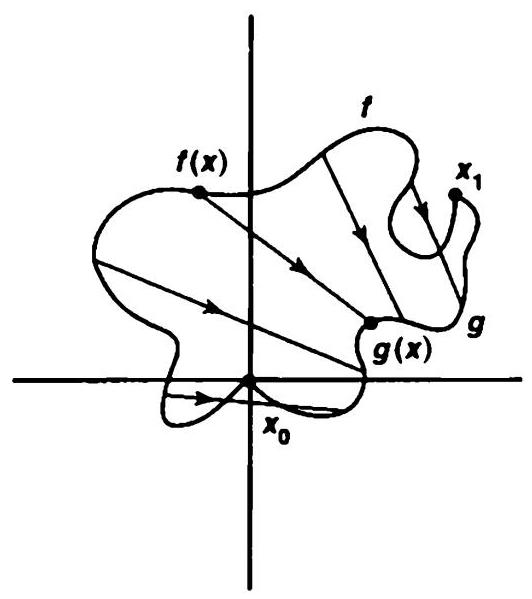
\includegraphics[width=0.4\textwidth]{images/51.3.jpg}
\end{center}
\hspace*{3em} 

Figure 51.3

\begin{center}
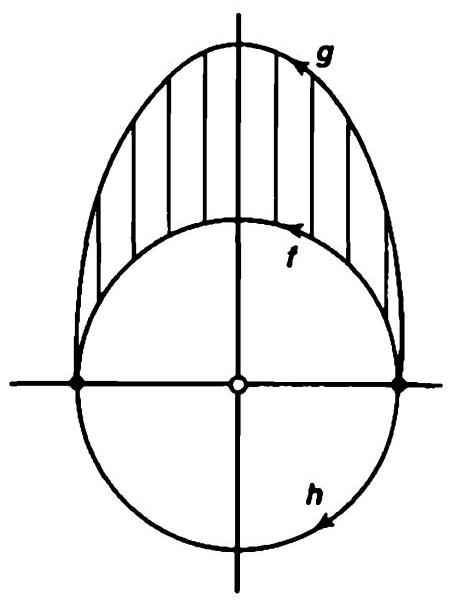
\includegraphics[width=0.4\textwidth]{images/51.4.jpg}
\end{center}
\hspace*{3em} 

Figure 51.4

\begin{centeredblock}
\begin{example}
	Let \(X\) denote the punctured plane, \({\mathbb{R}}^{2} - \{ 0\}\) , which we shall denote by \(\index{R@\({\mathbb{R}}^{2} - 0\)} \index{R@${\mathbb{R}}^{2} - 0$}{\mathbb{R}}^{2} - 0\) for short The following paths in \(X\) ,

\[
f( s)  = ( {\cos {\pi s},\sin {\pi s}}) ,
\]

\[
g( s)  = ( {\cos {\pi s},2\sin {\pi s}})
\]

are path homotopic, the straight-line homotopy between them is an acceptable path homotopy But the straight-line homotopy between \(f\) and the path

\[
h( s)  = ( {\cos {\pi s}, - \sin {\pi s}})
\]

is not acceptable, for its image does not lie in the space \(X = {\mathbb{R}}^{2} - 0\) . See Figure 51.4.

Indeed, there exists no path homotopy in \(X\) between paths \(f\) and \(h\) This result is hardly surprising, it is intuitively clear that one cannot ``deform \(f\) past the hole at 0 `` without introducing a discontinuity. But it takes some work to prove. We shall return to this example later

This example illustrates the fact that you must know what the range space is before you can tell whether two paths are path homotopic or not The paths \(f\) and \(h\) would be path homotopic if they were paths in \({\mathbb{R}}^{2}\)
\end{example}
\end{centeredblock}

Now we introduce some algebra into this geometric situation. We define a certain operation on \index{Path-homotopy class}s as follows:
\end{proof}
\begin{definition}
	If \(f\) is a path in \(X\) from \({x}_{0}\) to \({x}_{1}\) , and if \(g\) is a path in \(X\) from \({x}_{1}\) to \({x}_{2}\) , we define the product \(\index{f@\(f * g\)} \index{f@$f * g$}f * g\) of \(f\) and \(g\) to be the path \(h\) given by the equations

\[
h( s)  = \{  \begin{array}{ll} f( {2s}) & \text{ for }s \in  [  {0,\frac{1}{2}}]  , \\  g( {{2s} - 1}) & \text{ for }s \in  [  {\frac{1}{2},1}]  . \end{array}.
\]

The function \(h\) is well-defined and continuous, by the pasting lemma; it is a path in \(X\) from \({x}_{0}\) to \({x}_{2}\) . We think of \(h\) as the path whose first half is the path \(f\) and whose second half is the path \(g\) .
\end{definition}

The product operation on paths induces a well-defined operation on path-homotopy classes, defined by the equation

\[
[  f]   * [  g]   = [  {f * g}]
\]

To verify this fact, let \(F\) be a path homotopy between \(f\) and \({f}^{\prime }\) and let \(G\) be a path homotopy between \(g\) and \({g}^{\prime }\) . Define

\[
H( {s,t})  = \{  \begin{array}{ll} F( {{2s},t}) & \text{ for }s \in  [  {0,\frac{1}{2}}]  , \\  G( {{2s} - 1,t}) & \text{ for }s \in  [  {\frac{1}{2},1}]  . \end{array}.
\]

Because \(F( {1,t})  = {x}_{1} = G( {0,t})\) for all \(t\) , the map \(H\) is well-defined; it is continuous by the pasting lemma. You can check that \(H\) is the required path homotopy between \(f * g\) and \({f}^{\prime } * {g}^{\prime }\) It is pictured in Figure 51.5.

\begin{center}
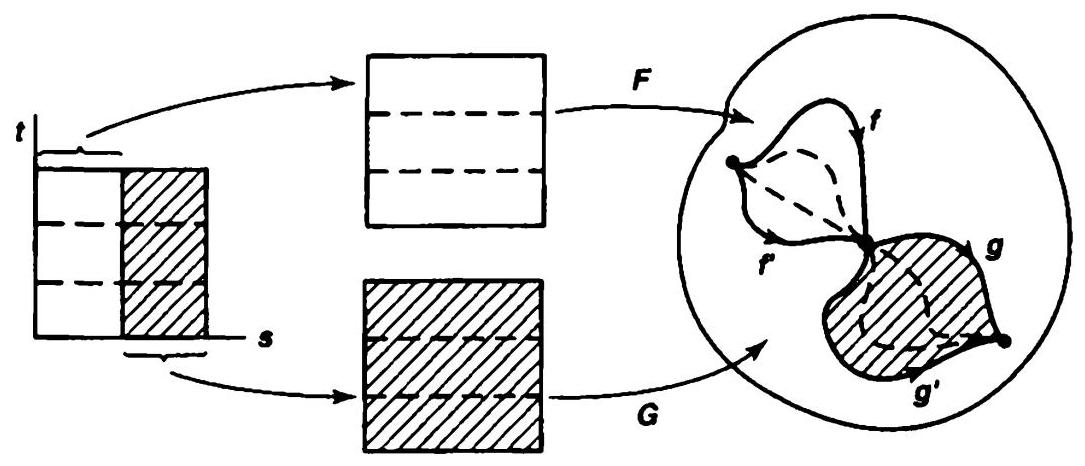
\includegraphics[width=1.0\textwidth]{images/51.5.jpg}
\end{center}
\hspace*{3em} 

Figure 51.5

The operation \(*\) on \index{path-homotopy class@Path-homotopy class}path-homotopy classes turns out to satisfy properties that look very much like the axioms for a group. They are called the \index{Groupoid properties} of \(*\) . One difference from the properties of a group is that \([  f]   * [  g]\) is not defined for every pair of classes, but only for those pairs \([  f]  ,[  g]\) for which \(f( 1)  = g( 0)\) .

\begin{theorem}
	The operation \(*\) has the following properties:

(I) (Associativity) If \([  f]   * ( {[  g]   * [  h]  })\) is defined, so is \(( {[  f]   * [  g]  })  * [  h]\) , and they are equal.

(2) (Right and left identities) Given \(x \in  X\) , let \(\index{e@\({e}_{x}\)} {e}_{x}\) denote the \index{Constant path} \({e}_{x} : I \rightarrow\)  \(X\) carrying all of \(I\) to the point \(x\) . If \(f\) is a path in \(X\) from \({x}_{0}\) to \({x}_{1}\) , then

\[
[  f]   * [  {e}_{{x}_{1}}]   = [  f]  \;\text{ and }\;[  {e}_{{x}_{0}}]   * [  f]   = [  f]  .
\]

(3) (Inverse) Given the path \(f\) in \(X\) from \({x}_{0}\) to \({x}_{1}\) , let \(\bar{f}\) be the path defined by \(\bar{f}( s)  = f( {1 - s})\) . It is called the reverse of \(f\) Then

\[
[  f]   * [  \bar{f}]   = [  {e}_{{x}_{0}}]  \;\text{ and }\;[  \bar{f}]   * [  f]   = [  {e}_{{x}_{1}}]  .
\]
\end{theorem}

\begin{proof}
	We shall make use of two elementary facts. The first is the fact that if \(k\) : \(X \rightarrow  Y\) is a continuous map, and if \(F\) is a path homotopy in \(X\) between the paths \(f\) and \({f}^{\prime }\) , then \(k \circ  F\) is a path homotopy in \(Y\) between the paths \(k \circ  f\) and \(k \circ  {f}^{\prime }\) . See Figure 51.6.
\begin{center}
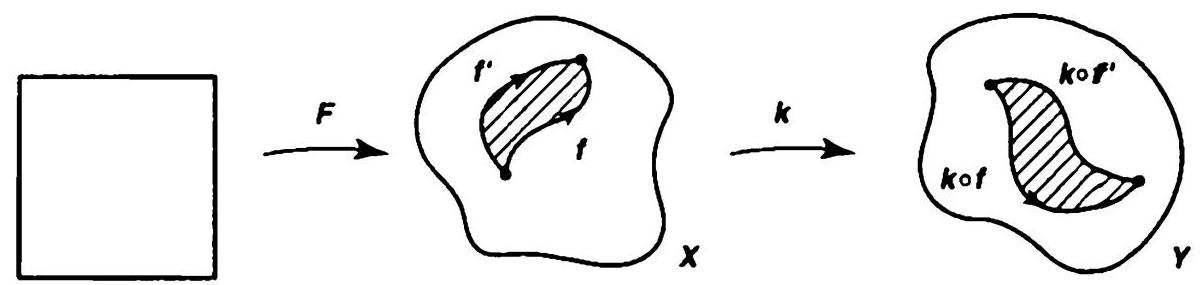
\includegraphics[width=1.0\textwidth]{images/51.6.jpg}
\end{center}
\hspace*{3em} 

Figure 51.6

The second is the fact that if \(k : X \rightarrow  Y\) is a continuous map and if \(f\) and \(g\) are paths in \(X\) with \(f( 1)  = g( 0)\) , then

\[
k \circ  ( {f * g})  = ( {k \circ  f})  * ( {k \circ  g}) .
\]

This equation follows at once from the definition of the product operation \(*\) .

Step 1. We verify properties (2) and (3). To verify (2), we let \({e}_{0}\) denote the \index{constant path@Constant path}constant path in \(I\) at 0, and we let \(i : I \rightarrow  I\) denote the identity map, which is a path in \(I\) from 0 to 1 . Then \({e}_{0} * i\) is also a path in \(I\) from 0 to 1 . (The graphs of these two paths are pictured in Figure 51.7.)

\begin{center}
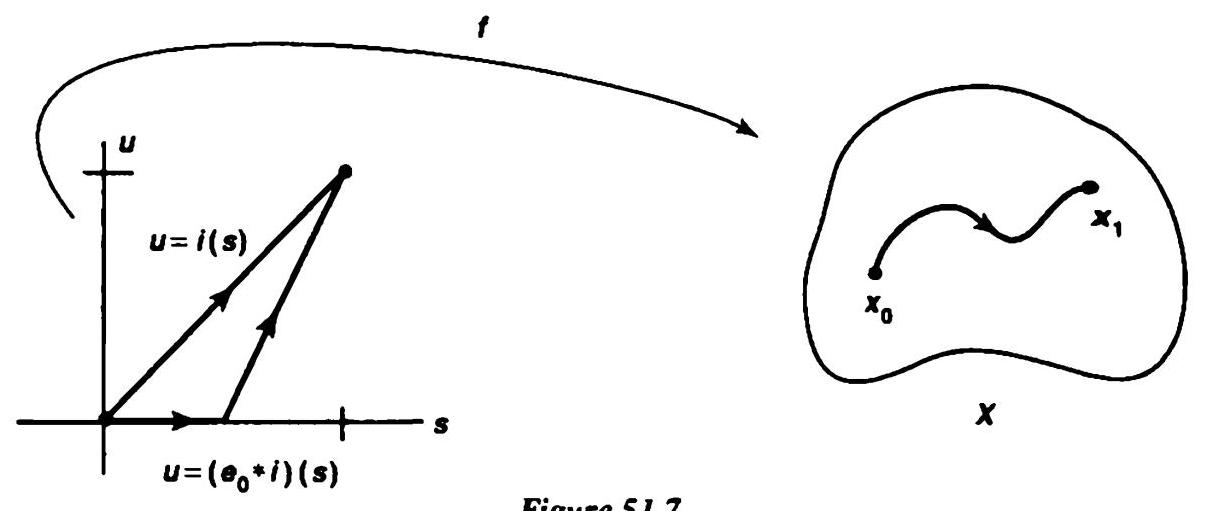
\includegraphics[width=1.0\textwidth]{images/51.7.jpg}
\end{center}
\hspace*{3em} 

Figure 51.7

Because \(I\) is convex, there is a path homotopy \(G\) in \(I\) between \(i\) and \({e}_{0} * i\) . Then \(f \circ  G\) is a path homotopy in \(X\) between the paths \(f \circ  i = f\) and

\[
f \circ  ( {{e}_{0} * i})  = ( {f \circ  {e}_{0}})  * ( {f \circ  i})  = {e}_{{x}_{0}} * f.
\]

An entirely similar argument, using the fact that if \({e}_{1}\) denotes the constant path at 1, then \(i * {e}_{1}\) is path homotopic in \(I\) to the path \(i\) , shows that \([  f]   * [  {e}_{{x}_{1}}]   = [  f]\) .

To verify (3), note that the reverse of \(i\) is \(\bar{i}( s)  = 1 - s\) . Then \(i * \bar{i}\) is a path in \(I\) beginning and ending at 0, and so is the constant path \({e}_{0}\) . (Their graphs are pictured in Figure 51.8.) Because \(I\) is convex, there is a path homotopy \(H\) in \(I\) between \({e}_{0}\) and \(i * \bar{i}\) . Then \(f \circ  H\) is a path homotopy between \(f \circ  {e}_{0} = {e}_{{x}_{0}}\) and

\[
( {f \circ  i})  * ( {f \circ  \bar{i}})  = f * \bar{f}.
\]

An entirely similar argument, using the fact that \(\bar{i} * i\) is path homotopic in \(I\) to \({e}_{1}\) , shows that \([  \bar{f}]   * [  f]   = [  {e}_{{x}_{1}}]\) .

\begin{center}
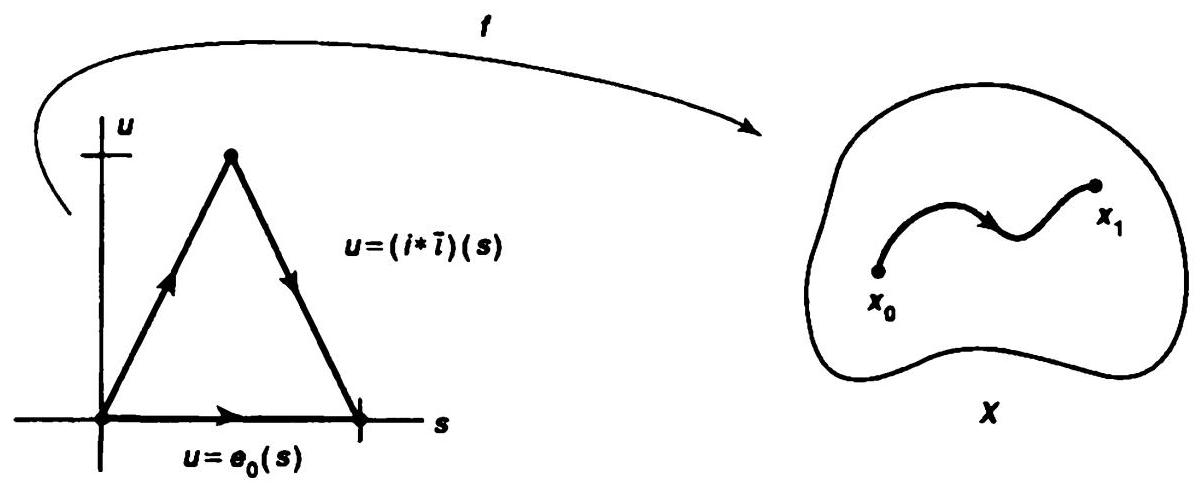
\includegraphics[width=1.0\textwidth]{images/51.8.jpg}
\end{center}
\hspace*{3em} 

Figure 51.8

Step 2. The proof of (1), associativity, is a bit trickier. For this proof, and for later use as well, it will be convenient to describe the product \(f * g\) in a different way.

If \([  {a,b}]\) and \([  {c,d}]\) are two intervals in \(\mathbb{R}\) , there is a unique map \(p : [  {a,b}]   \rightarrow  [  {c,d}]\) of the form \(p( x)  = {mx} + k\) that carries \(a\) to \(c\) and \(b\) to \(d\) ; we call it the \index{positive linear map: of intervals in@Positive linear map: of intervals in} positive linear map of \([  {a,b}]\) to \([  {c,d}]\) because its graph is a straight line with positive slope. Note that the inverse of such a map is another such map, and so is the \index{Covering map!composite}composite of two such maps.

With this terminology, the product \(f * g\) can be described as follows: \(\operatorname{On}[  {0,\frac{1}{2}}]\) , it equals the positive linear map of \([  {0,\frac{1}{2}}]\) to \([  {0,1}]\) , followed by \(f\) ; and on \([  {\frac{1}{2},1}]\) , it equals the positive linear map of \([  {\frac{1}{2},1}]\) to \([  {0,1}]\) , followed by \(g\) .

Now we verify (1). Given paths \(f,g\) , and \(h\) in \(X\) , the products \(f * ( {g * h})\) and \(( {f * g})  * h\) are defined precisely when \(f( 1)  = g( 0)\) and \(g( 1)  = h( 0)\) . Assuming these two conditions, we define also a ``triple product'' of the paths \(f,g\) , and \(h\) as follows: Choose points \(a\) and \(b\) of \(I\) so that \(0 < a < b < 1\) . Define a path \({k}_{a,b}\) in \(X\) as follows: On \([  {0,a}]\) it equals the positive linear map of \([  {0,a}]\) to \(I\) followed by \(f\) ; on \([  {a,b}]\) it equals the positive linear map of \([  {a,b}]\) to \(l\) followed by \(g\) ; and on \([  {b,1}]\) it equals the positive linear map of \([  {b,1}]\) to \(l\) followed by \(h\) . The path \({k}_{a,b}\) depends of course on the choice of the points \(a\) and \(b\) . But its path-homotopy class does not! We show that if \(c\) and \(d\) are another pair of points of \(I\) with \(0 < c < d < 1\) , then \({k}_{c,d}\) is path homotopic to \({k}_{a,b}\) .

Let \(p : I \rightarrow  I\) be the map whose graph is pictured in Figure 519. When restricted to \([  {0,a}]  ,[  {a,b}]\) , and \([  {b,1}]\) , respectively, it equals the positive linear maps of these intervals onto \([  {0,c}]  ,[  {c,d}]\) , and \([  {d,1}]\) , respectively. It follows at once that \({k}_{c,d} \circ  p\) equals \({k}_{a,b}\) . But \(p\) is a path in \(I\) from 0 to 1 ; and so is the identity map \(i : I \rightarrow  I\) . Hence, there is a path homotopy \(P\) in \(I\) between \(p\) and \(i\) . Then \({k}_{c,d} \circ  P\) is a path homotopy in \(X\) between \({k}_{a,b}\) and \({k}_{c,d}\)

\begin{center}
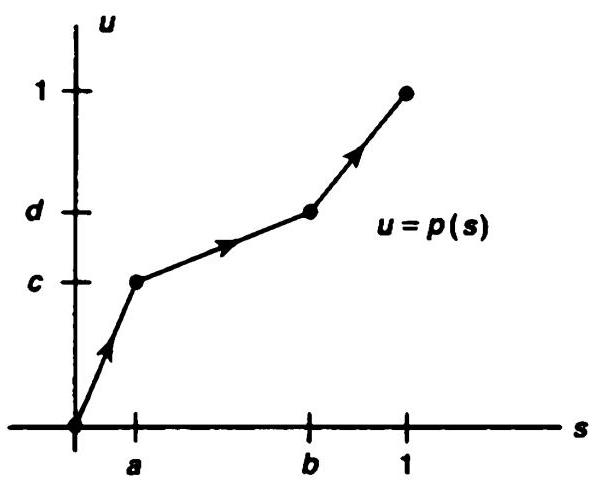
\includegraphics[width=0.5\textwidth]{images/51.9.jpg}
\end{center}
\hspace*{3em} 

Figure 51.9

What has this to do with associativity? A great deal. For the product \(f * ( {g * h})\) is exactly the triple product \({k}_{a,b}\) in the case where \(a = 1/2\) and \(b = 3/4\) , as you can check, while the product \(( {f * g})  * h\) equals \({k}_{c,d}\) in the case where \(c = 1/4\) and \(d = 1/2\) . Therefore these two products are path homotopic.

The argument just used to prove associativity goes through for any finite product \index{Product: of continuous maps!of paths}of paths. Roughly speaking, it says that as far as the path-homotopy class of the result is concerned, it doesn't matter how you chop up the interval when you form the product of paths! This result will be useful to us later, so we state it formally as a theorem here:
\end{proof}
\begin{theorem}
	Let \(f\) be a path in \(X\) , and let \({a}_{0},\ldots ,{a}_{n}\) be numbers such that \(0 = {a}_{0} < {a}_{1} < \cdots  < {a}_{n} = 1\) . Let \({f}_{i} : I \rightarrow  X\) be the path that equals the positive linear map of \(I\) onto \([  {{a}_{i - 1},{a}_{i}}]\) followed by \(f\) . Then

\[
[  f]   = [  {f}_{1}]   * \cdots  * [  {f}_{n}]  .
\]
\end{theorem}

\section*{Exercises}
\begin{enumerate}[itemsep=0.4em, parsep=0pt, topsep=0pt, partopsep=0pt, leftmargin=*, label=\arabic*., ref=\arabic*]
\item Show that if \(h,{h}^{\prime } : X \rightarrow  Y\) are homotopic and \(k,{k}^{\prime } : Y \rightarrow  Z\) are homotopic, then \(k \circ  h\) and \({k}^{\prime } \circ  {h}^{\prime }\) are homotopic.
\item Given spaces \(X\) and \(Y\) , let \(\index{X@\([  {X,Y}]\)}\) denote the set of homotopy classes of maps of \(X\) into \(Y\) .
  \begin{enumerate}[itemsep=0.2em, parsep=0pt, topsep=0pt, partopsep=0pt, leftmargin=*, label=(\alph*), align=left]
  \item Let \(I = [  {0,1}]\) . Show that for any \(X\) , the set \([  {X,I}]\) has a single element.
  \item Show that if \(Y\) is path connected, the set \([  {I,Y}]\) has a single element.
  \end{enumerate}
\item A space \(X\) is said to be contractible if the identity map \({i}_{X} : X \rightarrow  X\) is nulho-motopic.
  \begin{enumerate}[itemsep=0.2em, parsep=0pt, topsep=0pt, partopsep=0pt, leftmargin=*, label=(\alph*), align=left]
  \item Show that \(I\) and \(\mathbb{R}\) are contractible.
  \item Show that a \index{Contractible space} is path connected.
  \item Show that if \(Y\) is contractible, then for any \(X\) , the set \([  {X,Y}]\) has a single element.
  \item Show that if \(X\) is contractible and \(Y\) is path connected, then \([  {X,Y}]\) has a single element.
  \end{enumerate}
\end{enumerate}
\section*{§ 52 The Fundamental Group}

The set of path-homotopy classes of paths in a space \(X\) does not form a group under the operation \(*\) because the product of two path-homotopy classes is not always defined. But suppose we pick out a point \({x}_{0}\) of \(X\) to serve as a \index{Base point!effect on \({\pi }_{1}\)} ``\index{Base point}'' and restrict ourselves to those paths that begin and end at \({x}_{0}\) The set of these path-homotopy classes does form a group under \(*\) . It will be called the fundamental group of \(X\) .

In this section, we shall study the fundamental group and derive some of its properties. In particular, we shall show that the group is a topological invariant of the space \(X\) , the fact that is of crucial importance in using it to study homeomorphism problems.

Let us first review some terminology from group theory. Suppose \(G\) and \({G}^{\prime }\) are groups, written multiplicatively A \index{path-induced homomorphism@Path-induced homomorphism} homomorphism \(f : G \rightarrow  {G}^{\prime }\) is a map such that \(f( {x \cdot  y})  = f( x)  \cdot  f( y)\) for all \(x,y\) ; it automatically satisfies the equations \(f( e)  = {e}^{\prime }\) and \(f( {x}^{-1})  = f{( x) }^{-1}\) , where \(e\) and \({e}^{\prime }\) are the identities of \(G\) and \({G}^{\prime }\) , respectively, and the exponent -1 denotes the inverse. The \index{kernel of homomorphism@Kernel of homomorphism} kernel of \(f\) is the set \({f}^{-1}( {e}^{\prime })\) ; it is a subgroup of \(G\) . The image of \(f\) , similarly, is a subgroup of \({G}^{\prime }\) . The \index{homomorphism@Homomorphism}homomorphism \(f\) is called a \index{Monomorphism} if it is injective (or equivalently, if the kernel of \(f\) consists of \(e\) alone). It is called an \index{Epimorphism} if it is surjective; and it is called an isomorphism if it is bijective

Suppose \(G\) is a group and \(H\) is a subgroup of \(G\) . Let \({xH}\) denote the set of all products \({xh}\) , for \(h \in  H\) ; it is called a left coset of \(H\) in \(G\) . The collection of all such cosets forms a partition of \(G\) . Similarly, the collection of all \index{Right coset} \({Hx}\) of \(H\) in \(G\) forms a partition of \(G\) . We call \(H\) a \index{Normal subgroup} of \(G\) if \(x \cdot  h \cdot  {x}^{-1} \in  H\) for each \(x \in  G\) and each \(h \in  H\) . In this case, we have \({xH} = {Hx}\) for each \(x\) , so that our two partitions of \(G\) are the same. We denote this partition by \(G/H\) ; if one defines

\[
( {xH})  \cdot  ( {yH})  = ( {x \cdot  y}) H
\]

one obtains a well-defined operation on \(G/H\) that makes it a group. This group is called the quotient of \(G\) by \(H\) . The map \(f : G \rightarrow  G/H\) carrying \(x\) to \({xH}\) is an \index{epimorphism@Epimorphism}epimorphism with kernel \(H\) Conversely, if \(f : G \rightarrow  {G}^{\prime }\) is an epimorphism, then its kernel \(N\) is a \index{normal subgroup@Normal subgroup}normal subgroup of \(G\) , and \(f\) induces an isomorphism \(G/N \rightarrow  {G}^{\prime }\) that carries \({xN}\) to \(f( x)\) for each \(x \in  G\) .

If the subgroup \(H\) of \(G\) is not normal, it will still be convenient to use the symbol \(G/H\) ; we will use it to denote the collection of \index{right coset@Right coset}right cosets of \(H\) in \(G\) .

Now we define the fundamental group.

\begin{definition}
	Let \(X\) be a space; let \({x}_{0}\) be a point of \(X\) . A path in \(X\) that begins and ends at \({x}_{0}\) is called a \index{Loop} based at \({x}_{0}\) . The set of path homotopy classes of \index{loop@Loop}loops based at \({x}_{0}\) , with the operation \(*\) , is called the fundamental group of \(X\) relative to the \index{base point@Base point}base point \({x}_{0}\) . It is denoted by \(\index{pi@\({\pi }_{1}( {X,{x}_{0}})\)} {\pi }_{1}( {X,{x}_{0}})\) .
\end{definition}

It follows from Theorem 51.2 that the operation \(*\) , when restricted to this set, satisfies the axioms for a group. Given two loops \(f\) and \(g\) based at \({x}_{0}\) , the product \(f * g\) is always defined and is a loop based at \({x}_{0}\) . Associativity, the existence of an identity element \([  {e}_{{x}_{0}}]\) , and the existence of an inverse \([  \bar{f}]\) for \([  f]\) are immediate.

Sometimes this group is called the first homotopy group of \(X\) , which term implies that there is a second homotopy group. There are indeed groups \({\pi }_{n}( {X,{x}_{0}})\) for all \(n \in  {\mathbb{Z}}_{ + }\) , but we shall not study them in this book. They are part of the general subject called homotopy theory.

\begin{centeredblock}
\begin{example}
	Let \({\mathbb{R}}^{n}\) denote euclidean \(n\) -space. Then \({\pi }_{1}( {{\mathbb{R}}^{n},{x}_{0}})\) is the trivial group (the group consisting of the identity alone). For if \(f\) is a loop in \({\mathbb{R}}^{n}\) based at \({x}_{0}\) , the straight-line homotopy is a path homotopy between \(f\) and the constant path at \({x}_{0}\) . More generally, if \(X\) is any convex subset of \({\mathbb{R}}^{n}\) , then \({\pi }_{1}( {X,{x}_{0}})\) is the trivial group. In particular, the unit ball \({B}^{n}\) in \({\mathbb{R}}^{n}\) .

\[
{B}^{n} = \{  {\mathbf{x} \mid  {x}_{1}^{2} + \; + {x}_{n}^{2} \leq  1}\}  ,
\]

has trivial fundamental group.
\end{example}
\end{centeredblock}

An immediate question one asks is the extent to which the fundamental group depends on the base point. We consider that question now.

\begin{definition}
	Let \(\alpha\) be a path in \(X\) from \({x}_{0}\) to \({x}_{1}\) . We define a map

\[
\widehat{\alpha } : {\pi }_{1}( {X,{x}_{0}})  \rightarrow  {\pi }_{1}( {X,{x}_{1}})
\]

by the equation

\[
\widehat{\alpha }( [  f]  )  = [  \bar{\alpha }]   * [  f]   * [  \alpha ]  .
\]

The map \(\widehat{\alpha }\) , which we call `` \(\alpha\) -hat,'' is well-defined because the operation \(*\) is well-defined. If \(f\) is a loop based at \({x}_{0}\) , then \(\bar{\alpha } * ( {f * \alpha })\) is a loop based at \({x}_{1}\) . Hence \(\widehat{\alpha }\) maps \({\pi }_{1}( {X,{x}_{0}})\) into \({\pi }_{1}( {X,{x}_{1}})\) , as desired; note that it depends only on the path-homotopy class of \(\alpha\) . It is pictured in Figure 521.
\end{definition}

\begin{center}
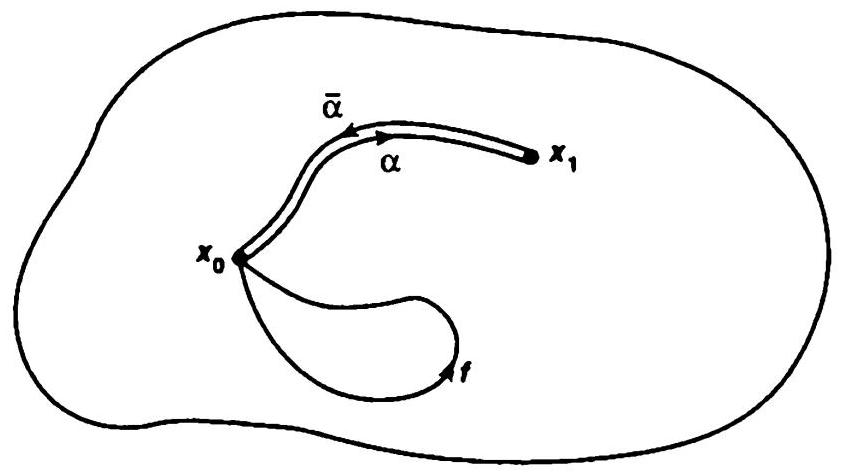
\includegraphics[width=0.7\textwidth]{images/52.1.jpg}
\end{center}
\hspace*{3em} 

Figure 52.1

\begin{theorem}
	The map \(\widehat{\alpha }\) is a group isomorphism.
\end{theorem}

\begin{proof}
	To show that \(\widehat{\alpha }\) is a homomorphism, we compute
\[
\widehat{\alpha }( [  f]  )  * \widehat{\alpha }( [  g]  )  = ( {[  \bar{\alpha }]   * [  f]   * [  \alpha ]  })  * ( {[  \bar{\alpha }]   * [  g]   * [  \alpha ]  })
\]

\[
= [  \bar{\alpha }]   * [  f]   * [  g]   * [  \alpha ]
\]

\[
= \widehat{\alpha }( {[  f]   * [  g]  }) \text{ . }
\]

To show that \(\widehat{\alpha }\) \index{alpha@\widehat{\alpha}!is an isomorphism}is an isomorphism, we show that if \(\beta\) denotes the path \(\bar{\alpha }\) , which is the reverse of \(\alpha\) , then \(\widehat{\beta }\) is an inverse for \(\widehat{\alpha }\) . We compute, for each element \([  h]\) of \({\pi }_{1}( {X,{x}_{1}})\) ,

\[
\widehat{\beta }( [  h]  )  = [  \bar{\beta }]   * [  h]   * [  \beta ]   = [  \alpha ]   * [  h]   * [  \bar{\alpha }]  ,
\]

\[
\widehat{\alpha }( {\widehat{\beta }( [  h]  ) })  = [  \bar{\alpha }]   * ( {[  \alpha ]   * [  h]   * [  \bar{\alpha }]  })  * [  \alpha ]   = [  h]  .
\]

A similar computation shows that \(\widehat{\beta }( {\widehat{\alpha }( [  f]  ) })  = [  f]\) for each \([  f]   \in  {\pi }_{1}( {X,{x}_{0}})\) .
\end{proof}
\begin{corollary}
	If \(X\) is path connected and \({x}_{0}\) and \({x}_{1}\) are two points of \(X\) , then \({\pi }_{1}( {X,{x}_{0}})\) is isomorphic to \({\pi }_{1}( {X,{x}_{1}})\) .
\end{corollary}

Suppose that \(X\) is a topological space. Let \(C\) be the path component of \(X\) containing \({x}_{0}\) It is easy to see that \({\pi }_{1}( {C,{x}_{0}})  = {\pi }_{1}( {X,{x}_{0}})\) , since all loops and homotopies in \(X\) that are based at \({x}_{0}\) must lie in the subspace \(C\) . Thus \({\pi }_{1}( {X,{x}_{0}})\) depends on only the path component of \(X\) containing \({x}_{0}\) ; it gives us no information whatever about the rest of \(X\) . For this reason, it is usual to deal with only path-connected spaces when studying the fundamental group

If \(X\) is path connected, all the groups \({\pi }_{1}( {X,x})\) are isomorphic, so it is tempting to try to ``identify'' all these groups with one another and to speak simply of the fundamental group of the space \(X\) , without reference to base point. The difficulty with this approach is that there is no natural way of identifying \({\pi }_{1}( {X,{x}_{0}})\) with \({\pi }_{1}( {X,{x}_{1}})\) ; different paths \(\alpha\) and \(\beta\) from \({x}_{0}\) to \({x}_{1}\) may give rise to different isomorphisms between these groups. For this reason, omitting the base point can lead to error.

It turns out that the isomorphism of \({\pi }_{1}( {X,{x}_{0}})\) with \({\pi }_{1}( {X,{x}_{1}})\) \index{alpha@\widehat{\alpha}!independent of path}is independent of path if and only if the fundamental group is abelian. (See Exercise 3.) This is a stringent requirement on the space \(X\) .

\begin{definition}
	A space \(X\) is said to be simply connected if it is a path-connected space and if \({\pi }_{1}( {X,{x}_{0}})\) is the trivial (one-element) group for some \({x}_{0} \in  X\) , and hence for every \({x}_{0} \in  X\) . We often express the fact that \({\pi }_{1}( {X,{x}_{0}})\) is the trivial group by writing \({\pi }_{1}( {X,{x}_{0}})  = 0.\)
\end{definition}

\begin{lemma}
	In a simply connected space \(X\) , any two paths having the same initial and final points are path homotopic.
\end{lemma}

\begin{proof}
	Let \(\alpha\) and \(\beta\) be two paths from \({x}_{0}\) to \({x}_{1}\) Then \(\alpha  * \bar{\beta }\) is defined and is a loop on \(X\) based at \({x}_{0}\) . Since \(X\) is simply connected, this loop is path homotopic to the constant loop at \({x}_{0}\) . Then
\[
[  {\alpha  * \bar{\beta }}]   * [  \dot{\beta }]   = [  {e}_{{x}_{0}}]   * [  \beta ]  ,
\]

from which it follows that \([  \alpha ]   = [  \beta ]\) .

It is intuitively clear that the fundamental group is a topological invariant of the space \(X\) . A convenient way to prove this fact formally is to introduce the notion of the ``homomorphism induced by a continuous map.''

Suppose that \(h : X \rightarrow  Y\) is a continuous map that carries the point \({x}_{0}\) of \(X\) to the point \({y}_{0}\) of \(Y\) . We often denote this fact by writing

\[
h : ( {X,{x}_{0}})  \rightarrow  ( {Y,{y}_{0}}) .
\]

If \(f\) is a loop in \(X\) based at \({x}_{0}\) , then the composite \(h \circ  f : I \rightarrow  Y\) is a loop in \(Y\) based at \({y}_{0}\) . The correspondence \(f \rightarrow  h \circ  f\) thus gives rise to a map carrying \({\pi }_{1}( {X,{x}_{0}})\) into \({\pi }_{1}( {Y,{y}_{0}})\) . We define it formally as follows:
\end{proof}
\begin{definition}
	Let \(h.( {X,{x}_{0}})  \rightarrow  ( {Y,{y}_{0}})\) be a continuous map. Define

\[
\index{h@\({h}_{ * }\)} {h}_{ * }.{\pi }_{1}( {X,{x}_{0}})  \rightarrow  {\pi }_{1}( {Y,{y}_{0}})
\]

by the equation

\[
{h}_{ * }( [  f]  )  = [  {h \circ  f}]  \text{ . }
\]

The map \({h}_{ * }\) is called the homomorphism induced by \(h\) , relative to the base point \({x}_{0}\) .
\end{definition}

The map \({h}_{ * }\) is well-defined, for if \(F\) is a path homotopy between the paths \(f\) and \({f}^{\prime }\) , then \(h \circ  F\) is a path homotopy between the paths \(h \circ  f\) and \(h \circ  {f}^{\prime }\) . The fact that \({h}_{ * }\) is a homomorphism follows from the equation

\[
( {h \circ  f})  * ( {h \circ  g})  = h \circ  ( {f * g}) .
\]

The homomorphism \({h}_{ * }\) depends not only on the map \(h : X \rightarrow  Y\) but also on the choice of the base point \({x}_{0}\) . (Once \({x}_{0}\) is chosen, \({y}_{0}\) is determined by \(h\) .) So some notational difficulty will arise if we want to consider several different base points for \(X\) . If \({x}_{0}\) and \({x}_{1}\) are two different points of \(X\) , we cannot use the same symbol \({h}_{ * }\) to stand for two different homomorphisms, one having domain \({\pi }_{1}( {X,{x}_{0}})\) and the other having domain \({\pi }_{1}( {X,{x}_{1}})\) . Even if \(X\) is path connected, so these groups are isomorphic, they are still not the same group. In such a case, we shall use the notation

\[
{( {h}_{{x}_{0}}) }_{ * } : {\pi }_{1}( {X,{x}_{0}})  \rightarrow  {\pi }_{1}( {Y,{y}_{0}})
\]

for the first homomorphism and \({( {h}_{{x}_{1}}) }_{ * }\) for the second. If there is only one \index{Base point!effect on \({h}_{ * }\)}base point under consideration, we shall omit mention of the base point and denote the induced homomorphism merely by \({h}_{ * }\) .

The induced homomorphism has two properties that are crucial in the applications. They are called its ``\index{\({h}_{ * }\)!functorial properties}functorial properties'' and are given in the following theorem:

\begin{theorem}
	If \(h : ( {X,{x}_{0}})  \rightarrow  ( {Y,{y}_{0}})\) and \(k : ( {Y,{y}_{0}})  \rightarrow  ( {Z,{z}_{0}})\) are continuous, then \({( k \circ  h) }_{ * } = {k}_{ * } \circ  {h}_{ * }\) If \(i : ( {X,{x}_{0}})  \rightarrow  ( {X,{x}_{0}})\) is the identity map, then \({i}_{ * }\) is the identity homomorphism.
\end{theorem}

\begin{proof}
	The proof is a triviality. By definition,
\[
{( k \circ  h) }_{ * }( [  f]  )  = [  {( {k \circ  h})  \circ  f}]  ,
\]

\[
( {{k}_{ * } \circ  {h}_{ * }}) ( [  f]  )  = {k}_{ * }( {{h}_{ * }( [  f]  ) })  = {k}_{ * }( [  {h \circ  f}]  )  = [  {k \circ  ( {h \circ  f}) }]  .
\]

Similarly, \({i}_{ * }( [  f]  )  = [  {i \circ  f}]   = [  f]\)
\end{proof}
\begin{corollary}
	If \(h : ( {X,{x}_{0}})  \rightarrow  ( {Y,{y}_{0}})\) is a homeomorphism of \(X\) with \(Y\) , then \({h}_{ * }\) is an isomorphism of \({\pi }_{1}( {X,{x}_{0}})\) with \({\pi }_{1}( {Y,{y}_{0}})\) .
\end{corollary}

\begin{proof}
	Let \(k \cdot  ( {Y,{y}_{0}})  \rightarrow  ( {X,{x}_{0}})\) be the inverse of \(h\) . Then \({k}_{ * } \circ  {h}_{ * } = {( k \circ  h) }_{ * } = {i}_{ * }\) , where \(i\) is the identity map of \(( {X,{x}_{0}})\) ; and \({h}_{ * } \circ  {k}_{ * } = {( h \circ  k) }_{ * } = {j}_{ * }\) , where \(j\) is the identity map of \(( {Y,{y}_{0}})\) . Since \({i}_{ * }\) and \({j}_{ * }\) are the identity homomorphisms of the groups \({\pi }_{1}( {X,{x}_{0}})\) and \({\pi }_{1}( {Y,{y}_{0}})\) , respectively, \({k}_{ * }\) is the inverse of \({h}_{ * }\) .
\end{proof}
\section*{Exercises}
\begin{enumerate}[itemsep=0.4em, parsep=0pt, topsep=0pt, partopsep=0pt, leftmargin=*, label=\arabic*., ref=\arabic*]
\item A subset \(A\) of \({\mathbb{R}}^{n}\) is said to be \index{star-convex set@Star-convex set} star convex if for some point \({a}_{0}\) of \(A\) , all the line segments joining \({a}_{0}\) to other points of \(A\) lie in \(A\) .
  \begin{enumerate}[itemsep=0.2em, parsep=0pt, topsep=0pt, partopsep=0pt, leftmargin=*, label=(\alph*), align=left]
  \item Find a star convex set that is not convex.
  \item Show that if \(A\) is star convex, \(A\) is simply connected.
  \end{enumerate}
\item Let \(\alpha\) be a path in \(X\) from \({x}_{0}\) to \({x}_{1}\) ; let \(\beta\) be a path in \(X\) from \({x}_{1}\) to \({x}_{2}\) . Show that if \(\gamma  = \alpha  * \beta\) , then \(\widehat{\gamma } = \widehat{\beta } \circ  \widehat{\alpha }\) .
\item Let \({x}_{0}\) and \({x}_{1}\) be points of the path-connected space \(X\) . Show that \({\pi }_{1}( {X,{x}_{0}})\) is abelian if and only if for every pair \(\alpha\) and \(\beta\) of paths from \({x}_{0}\) to \({x}_{1}\) , we have \(\widehat{\alpha } = \widehat{\beta }\) .
\item Let \(A \subset  X\) ; suppose \(r : X \rightarrow  A\) is a continuous map such that \(r( a)  = a\) for each \(a \in  A\) . (The map \(r\) is called a \index{Retraction} of \(X\) onto \(A\) ) If \({a}_{0} \in  A\) , show that \[ {r}_{ * } : {\pi }_{1}( {X,{a}_{0}})  \rightarrow  {\pi }_{1}( {A,{a}_{0}}) \] is surjective.
\item Let \(A\) be a subspace of \({\mathbb{R}}^{n}\) ; let \(h : ( {A,{a}_{0}})  \rightarrow  ( {Y,{y}_{0}})\) . Show that if \(h\) is extendable to a continuous map of \({\mathbb{R}}^{n}\) into \(Y\) , then \({h}_{ * }\) is the \index{Trivial homomorphism} (the homomorphism that maps everything to the identity element).
\item Show that if \(X\) is path connected, the homomorphism induced by a continuous map is independent of base point, up to isomorphisms of the groups involved. More precisely, let \(h : X \rightarrow  Y\) be continuous, with \(h( {x}_{0})  = {y}_{0}\) and \(h( {x}_{1})  = {y}_{1}\) . Let \(\alpha\) be a path in \(X\) from \({x}_{0}\) to \({x}_{1}\) , and let \(\beta  = h \circ  \alpha\) . Show that \[ \widehat{\beta } \circ  {( {h}_{{x}_{0}}) }_{ * } = {( {h}_{{x}_{1}}) }_{ * } \circ  \widehat{\alpha }. \] This equation expresses the fact that the following diagram of maps ``commutes.'' \begin{center} 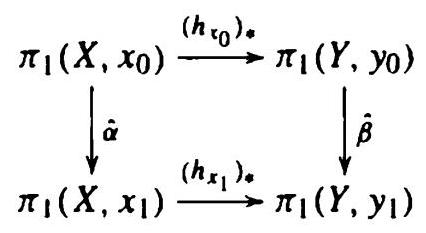
\includegraphics[width=0.3\textwidth]{images/52.2.jpg} \end{center} \hspace*{3em}
\item Let \(G\) be a topological group with operation - and identity element \({x}_{0}\) Let \(\Omega ( {G,{x}_{0}})\) denote the set of all loops in \(G\) based at \({x}_{0}\) . If \(f,g \in  \Omega ( {G,{x}_{0}})\) , let us define a loop \(f \otimes  g\) by the rule \[ ( {f \otimes  g}) ( s)  = f( s)  \cdot  g( s) . \]
  \begin{enumerate}[itemsep=0.2em, parsep=0pt, topsep=0pt, partopsep=0pt, leftmargin=*, label=(\alph*), align=left]
  \item Show that this operation makes the set \(\Omega ( {G,{x}_{0}})\) into a group.
  \item Show that this operation induces a group operation \(\otimes\) on \({\pi }_{1}( {G,{x}_{0}})\) .
  \item Show that the two group operations \(*\) and \(\otimes\) on \({\pi }_{1}( {G,{x}_{0}})\) are the same. [Hint: Compute \(( {f * {e}_{{x}_{0}}})  \otimes  ( {{e}_{{x}_{0}} * g})\) ]
  \item Show that \({\pi }_{1}( {G,{x}_{0}})\) is abelian.
  \end{enumerate}
\end{enumerate}
\section*{§ 53 Covering Spaces}

\index{covering space@Covering Space} We have shown that any convex subspace of \({\mathbb{R}}^{n}\) has a trivial fundamental group; we turn now to the task of computing some fundamental groups that are not trivial. One of the most useful tools for this purpose is the notion of \index{covering space@Covering space}covering space, which we introduce in this section. \index{\({S}^{1}\)!covering spaces}Covering spaces are also important in the study of Riemann surfaces and complex \index{prüfer manifold@Prüfer manifold} manifolds. (See 		\cite{AhlforsSario1960}.) We shall study them in more detail in Chapter 13. Definition. Let \(p\;E \rightarrow  B\) be a continuous surjective map. The open set \(U\) of \(B\) is said to be \index{Evenly covered} by \(p\) if the inverse image \({p}^{-1}( U)\) can be written as the union of disjoint open sets \({V}_{\alpha }\) in \(E\) such that for each \(\alpha\) , the \index{restriction: of a covering map@Restriction: of a covering map} restriction of \(p\) to \({V}_{\alpha }\) is a homeomorphism of \({V}_{\alpha }\) onto \(U\) The collection \(\{  {V}_{\alpha }\}\) will be called a partition of \({p}^{-1}( U)\) into \index{slice: in covering space@Slice: in covering space} slices

If \(U\) is an open set that is evenly covered by \(p\) , we often picture the set \({p}^{-1}( U)\) as a ``stack of pancakes,'' each having the same size and shape as \(U\) , floating in the arr above \(U\) ; the map \(p\) squashes them all down onto \(U\) . See Figure 53.1. Note that if \(U\) is \index{evenly covered@Evenly covered}evenly covered by \(p\) and \(W\) is an open set contained in \(U\) , then \(W\) is also evenly covered by \(p\) .

\begin{center}
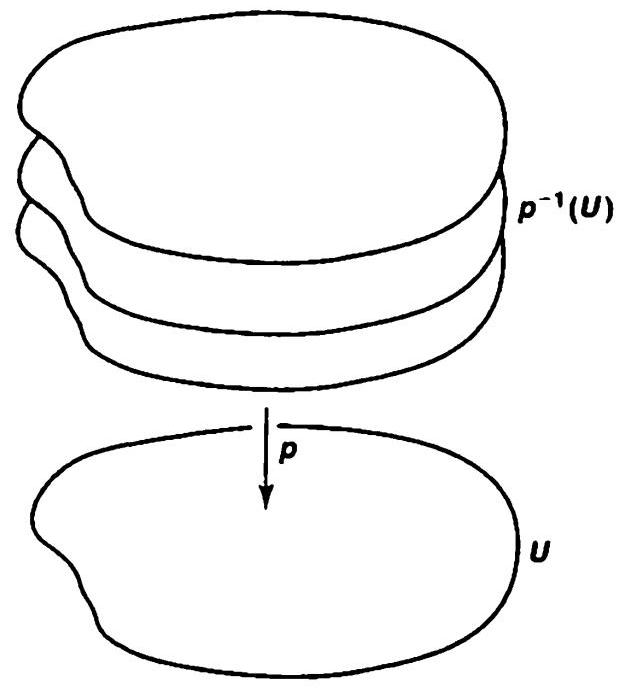
\includegraphics[width=0.5\textwidth]{images/53.1.jpg}
\end{center}
\hspace*{3em} 

Figure 53.1

\begin{definition}
	Let \(p : B \rightarrow  B\) be continuous and surjective. If every point \(b\) of \(B\) has a neighborhood \(U\) that is evenly covered by \(p\) , then \(p\) is called a \index{Covering map}, and \(E\) is said to be a covering space of \(B\)
\end{definition}

Note that if \(p : E \rightarrow  B\) is a covering map, then for each \(b \in  B\) the subspace \({p}^{-1}( b)\) of \(E\) has the discrete topology For each slice \({V}_{\alpha }\) \index{Covering map!is open}is open in \(E\) and intersects the set \({p}^{-1}( b)\) in a single point; therefore, this point is open in \({p}^{-1}( b)\) .

Note also that if \(p : E \rightarrow  B\) is a \index{covering map@Covering map}covering map, then \(p\) is an open map. For suppose \(A\) is an open set of \(E\) . Given \(x \in  p( A)\) , choose a neighborhood \(U\) of \(x\) that is evenly covered by \(p\) Let \(\{  {V}_{\alpha }\}\) be a partition of \({p}^{-1}( U)\) into slices. There is a point \(y\) of \(A\) such that \(p( y)  = x\) ; let \({V}_{\beta }\) be the slice containing \(y\) . The set \({V}_{\beta } \cap  A\) is open in \(E\) and hence open in \({V}_{\beta }\) , because \(p\) maps \({V}_{\beta }\) homeomorphically onto \(U\) , the set \(p( {{V}_{\beta } \cap  A})\) is open in \(U\) and hence open in \(B\) ; it is thus a neighborhood of \(x\) contained in \(p( A)\) , as desired.

\begin{centeredblock}
\begin{example}
	Let \(X\) be any space; let \(i : X \rightarrow  X\) be the identity map. Then \(i\) is a covering map (of the most trivial sort). More generally, let \(E\) be the space \(X \times  \{ 1,\ldots ,n\}\) consisting of \(n\) disjoint copies of \(X\) . The map \(p : E \rightarrow  X\) given by \(p( {x,i})  = x\) for all \(i\) is again a (rather trivial) covering map. In this case, we can picture the entire space \(E\) as a stack of pancakes over \(X\) .
\end{example}
\end{centeredblock}

In practice, one often restricts oneself to covering spaces that are path connected, to eliminate trivial coverings of the pancake-stack variety. An example of such a nontrivial covering space is the following.

\begin{theorem}
	The map \(p.\mathbb{R} \rightarrow  {S}^{1}\) given by the equation

\[
p( x)  = ( {\cos {2\pi x},\sin {2\pi x}})
\]

is a covering map.
\end{theorem}

One can picture \(p\) as a function that wraps the real line \(\mathbb{R}\) around the circle \({S}^{1}\) , and in the process maps each interval \([  {n,n + 1}]\) onto \({S}^{1}\) .

\begin{proof}
	The fact that \(p\) is a covering map comes from elementary properties of the sine and cosine functions. Consider, for example, the subset \(U\) of \({S}^{1}\) consisting of those points having positive first coordinate. The set \({p}^{-1}( U)\) consists of those points \(x\) for which \(\cos {2\pi x}\) is positive, that is, it is the union of the intervals
\[
{V}_{n} = ( {n - \frac{1}{4},n + \frac{1}{4}})
\]

for all \(n \in  \mathbb{Z}\) . See Figure 53.2. Now, restricted to any closed interval \({\bar{V}}_{n}\) , the map \(p\) is injective because \(\sin {2\pi x}\) is strictly monotonic on such an interval. Furthermore, \(p\) carries \({\bar{V}}_{n}\) surjectively onto \(U\) , and \({V}_{n}\) to \(U\) , by the intermediate value theorem. Since \({\bar{V}}_{n}\) is compact, \(p \mid  {\bar{V}}_{n}\) is a homeomorphism of \({\bar{V}}_{n}\) with \(\bar{U}\) . In particular, \(p \mid  {V}_{n}\) is a homeomorphism of \({V}_{n}\) with \(U\)

\begin{center}
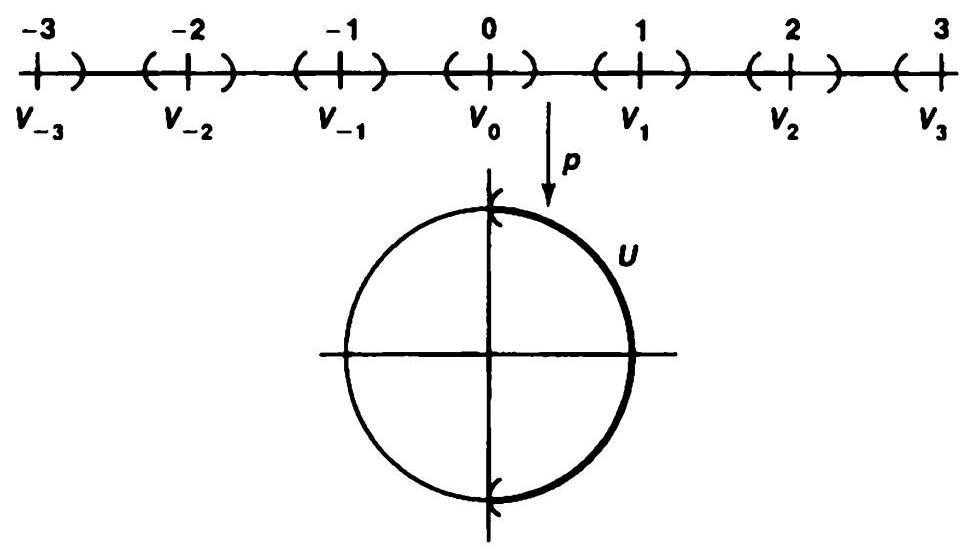
\includegraphics[width=0.8\textwidth]{images/53.2.jpg}
\end{center}
\hspace*{3em} 

Figure 53.2

Similar arguments can be applied to the intersections of \({S}^{1}\) with the upper and lower open half-planes, and with the open left-hand half-plane. These open sets cover \({S}^{1}\) , and each of them is evenly covered by \(p\) . Hence \(p : \mathbb{R} \rightarrow  {S}^{1}\) is a covering map.

If \(p : E \rightarrow  B\) is a covering map, then \(p\) is a \index{Local homeomorphism} of \(E\) with \(B\) . That is, each point \(e\) of \(E\) has a neighborhood that is mapped homeomorphically by \(p\) onto an open subset of \(B\) . The condition that \(p\) be a local homeomorphism does not suffice, however, to ensure that \(p\) is a covering map, as the following example shows.

\begin{centeredblock}
\begin{example}
	The map \(p : {\mathbb{R}}_{ + } \rightarrow  {S}^{1}\) given by the equation

\[
p( x)  = ( {\cos {2\pi x},\sin {2\pi x}})
\]

is surjective, and it is a \index{local homeomorphism@Local homeomorphism}local homeomorphism. See Figure 53.3. But it is not a covering map, for the point \({b}_{0} = ( {1,0})\) has no neighborhood \(U\) that is evenly covered by \(p\) . The typical neighborhood \(U\) of \({b}_{0}\) has an inverse image consisting of small neighborhoods \({V}_{n}\) of each integer \(n\) for \(n > 0\) , along with a small interval \({V}_{0}\) of the form \(( {0,\epsilon })\) . Each of the intervals \({V}_{n}\) for \(n > 0\) is mapped homeomorphically onto \(U\) by the map \(p\) , but the interval \({V}_{0}\) is only imbedded in \(U\) by \(p\) .

\begin{center}
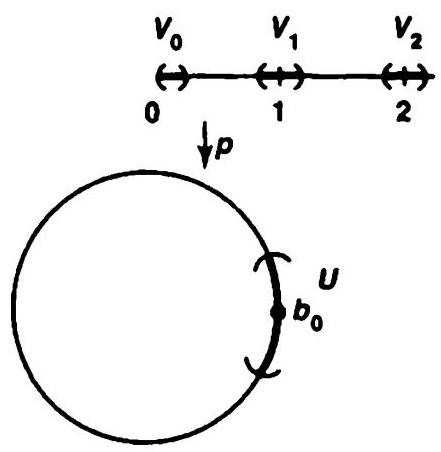
\includegraphics[width=0.4\textwidth]{images/53.3.jpg}
\end{center}
\hspace*{3em} 

Figure 53.3

\end{example}
\end{centeredblock}

\begin{centeredblock}
\begin{example}
	The preceding example might lead you to think that the real line \(\mathbb{R}\) is the only connected covering space of the circle \({S}^{1}\) . This is not so. Consider, for example, the map \(p.{S}^{1} \rightarrow  {S}^{1}\) given in equations by

\[
p( z)  = {z}^{2}.
\]

[Here we consider \({S}^{1}\) as the subset of the complex plane \(\mathbb{C}\) consisting of those complex numbers \(z\) with \(| z|  = 1\) ] We leave it to you to check that \(p\) is a covering map.
\end{example}
\end{centeredblock}

Example 2 shows that the map obtained by restricting a covering map may not be a covering map. Here is one situation where it will be a covering map:
\end{proof}
\begin{theorem}
	Let \(p : E \rightarrow  B\) be a covering map. If \({B}_{0}\) is a subspace of \(B\) , and if \({E}_{0} = {p}^{-1}( {B}_{0})\) , then the map \({p}_{0} : {E}_{0} \rightarrow  {B}_{0}\) obtained by restricting \(p\) is a covering map.
\end{theorem}

\begin{proof}
	Given \({b}_{0} \in  {B}_{0}\) , let \(U\) be an open set in \(B\) containing \({b}_{0}\) that is evenly covered by \(p\) ; let \(\{  {V}_{\alpha }\}\) be a partition of \({p}^{-1}( U)\) into slices. Then \(U \cap  {B}_{0}\) is a neighborhood of \({b}_{0}\) in \({B}_{0}\) , and the sets \({V}_{\alpha } \cap  {E}_{0}\) are disjoint open sets in \({E}_{0}\) whose union is \({p}^{-1}( {U \cap  {B}_{0}})\) , and each is mapped homeomorphically onto \(U \cap  {B}_{0}\) by \(p\) .
\end{proof}
\begin{theorem}
	If \(p : E \rightarrow  B\) and \({p}^{\prime } : {E}^{\prime } \rightarrow  {B}^{\prime }\) are covering maps, then

\[
p \times  {p}^{\prime } : E \times  {E}^{\prime } \rightarrow  B \times  {B}^{\prime }
\]

is a covering map.
\end{theorem}

\begin{proof}
	Given \(b \in  B\) and \({b}^{\prime } \in  {B}^{\prime }\) , let \(U\) and \({U}^{\prime }\) be neighborhoods of \(b\) and \({b}^{\prime }\) , respectively, that are evenly covered by \(p\) and \({p}^{\prime }\) , respectively. Let \(\{  {V}_{\alpha }\}\) and \(\{  {V}_{\beta }^{\prime }\}\) be partitions of \({p}^{-1}( U)\) and \({( {p}^{\prime }) }^{-1}( {U}^{\prime })\) , respectively, into slices. Then the inverse image under \(p \times  {p}^{\prime }\) of the open set \(U \times  {U}^{\prime }\) is the union of all the sets \({V}_{\alpha } \times  {V}_{\beta }^{\prime }\) . These are disjoint open sets of \(E \times  {E}^{\prime }\) , and each is mapped homeomorphically onto \({U}^{\prime } \times  {U}^{\prime }\) by \(p \times  {p}^{\prime }\) .

\begin{centeredblock}
\begin{example}
	Consider the space \(T = {S}^{1} \times  {S}^{1}\) , it is called the torus The product map

\[
p \times  p\mathbb{R} \times  \mathbb{R} \rightarrow  {S}^{1} \times  {S}^{1}
\]

is a covering of the torus by the plane \({\mathbb{R}}^{2}\) , where \(p\) denotes the covering map of Theorem 53 1 Each of the unit squares \([  {n,n + 1}]   \times  [  {m,m + 1}]\) gets wrapped by \(p \times  p\) entirely around the torus. See Figure 534

\begin{center}
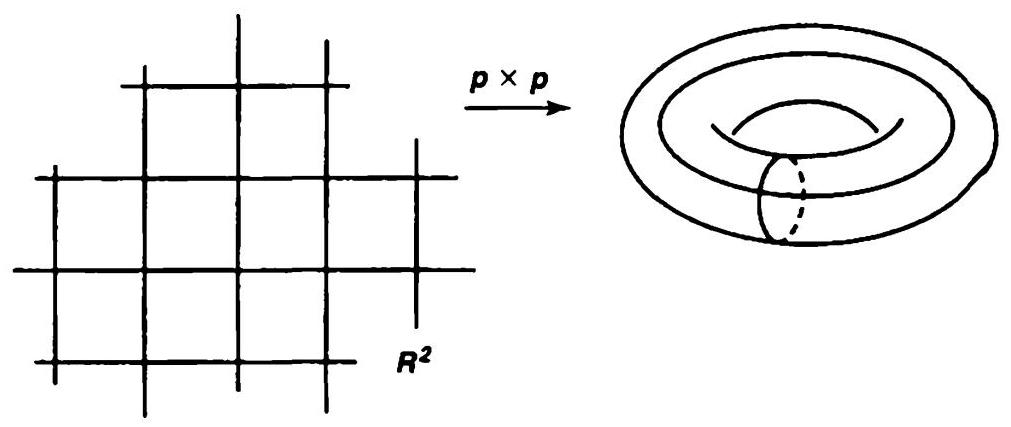
\includegraphics[width=0.9\textwidth]{images/53.4.jpg}
\end{center}
\hspace*{3em} 

Figure 53.4

In this figure, we have pictured the torus not as the product \({S}^{1} \times  {S}^{1}\) , which is a subspace of \({\mathbb{R}}^{4}\) and thus difficult to visualize, but as the familiar doughnut-shaped surface \(D\) in \({\mathbb{R}}^{3}\) obtained by rotating the circle \({C}_{1}\) in the \({xz}\) -plane of radius \(\frac{1}{3}\) centered at(1,0,0)about the \(z\) -axis. It is not hard to see that \({S}^{1} \times  {S}^{1}\) is homeomorphic with the surface \(D\) Let \({C}_{2}\) be the circle of radius 1 in the \({xy}\) -plane centered at the origin. Then let us map \({C}_{1} \times  {C}_{2}\) into \(D\) by defining \(f( {a \times  b})\) to be that point into which \(a\) is carried when one rotates the circle \({C}_{1}\) about the \(z\) -axis until its center hits the point \(b\) See Figure 53.5. The map \(f\) will be a homeomorphism of \({C}_{1} \times  {C}_{2}\) with \(D\) , as you can check mentally. If you wish, you can write equations for \(f\) and check continuity, injectivity, and surjectivity directly. (Continuity of \({f}^{-1}\) will follow from compactness of \({C}_{1} \times  {C}_{2}\) .)

\begin{center}
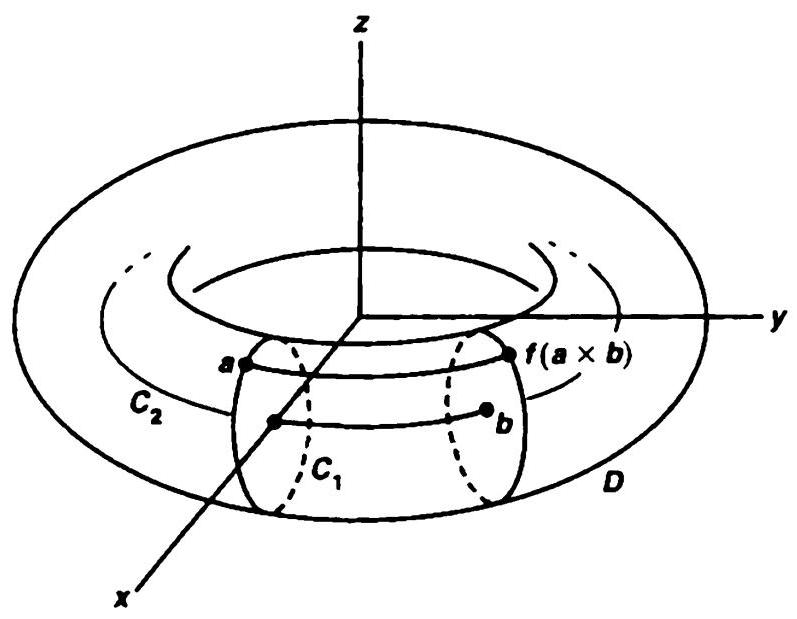
\includegraphics[width=0.7\textwidth]{images/53.5.jpg}
\end{center}
\hspace*{3em} 

Figure 53.5

\end{example}
\end{centeredblock}

\begin{centeredblock}
\begin{example}
	Consider the covering map \(p \times  p\) of the preceding example. Let \({b}_{0}\) denote the point \(p( 0)\) of \({S}^{1}\) ; and let \({B}_{0}\) denote the subspace

\[
{B}_{0} = ( {{S}^{1} \times  {b}_{0}})  \cup  ( {{b}_{0} \times  {S}^{1}})
\]

of \({S}^{1} \times  {S}^{1}\) . Then \({B}_{0}\) is the union of two circles that have a point in common, we sometimes call it the \index{Figure-eight space} The space \({E}_{0} = {p}^{-1}( {B}_{0})\) is the ``infinite grid''

\[
{E}_{0} = ( {\mathbb{R} \times  \mathbb{Z}})  \cup  ( {\mathbb{Z} \times  \mathbb{R}})
\]

pictured in Figure 534. The map \({p}_{0} : {E}_{0} \rightarrow  {B}_{0}\) obtained by restricting \(p \times  p\) is thus a covering map.

The infinite grid is but one \index{Torus!covering space of}covering space of the figure eight; we shall see others later on.

\end{example}
\end{centeredblock}

\begin{centeredblock}
\begin{example}
	Consider the covering map

\[
p \times  i : \mathbb{R} \times  {\mathbb{R}}_{ + } \rightarrow  {S}^{1} \times  {\mathbb{R}}_{ + }
\]

where \(i\) is the identity map of \({\mathbb{R}}_{ + }\) and \(p\) is the map of Theorem 531. If we take the standard homeomorphism of \({S}^{1} \times  {\mathbb{R}}_{ + }\) with \({\mathbb{R}}^{2} - \mathbf{0}\) , sending \(x \times  t\) to \({tx}\) , the composite gives us a covering

\[
\mathbb{R} \times  {\mathbb{R}}_{ + } \rightarrow  {\mathbb{R}}^{2} - 0
\]

of the punctured plane by the open upper half-plane. It is pictured in Figure S3.6. This covering map appears in the study of complex variables as the Riemann surface corresponding to the complex logarithm function.

\begin{center}
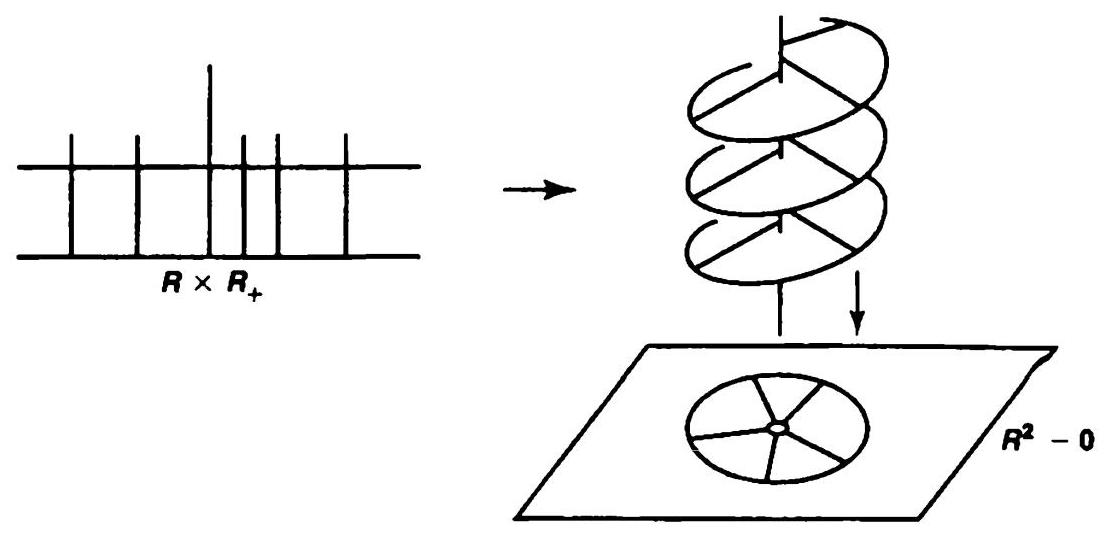
\includegraphics[width=1.0\textwidth]{images/53.6.jpg}
\end{center}
\hspace*{3em} 

Figure 53.6
\end{example}
\end{centeredblock}
\end{proof}
\section*{Exercises}
\begin{enumerate}[itemsep=0.4em, parsep=0pt, topsep=0pt, partopsep=0pt, leftmargin=*, label=\arabic*., ref=\arabic*]
\item Let \(Y\) have the discrete topology. Show that if \(p : X \times  Y \rightarrow  X\) is projection on the first coordinate, then \(p\) is a covering map.
\item Let \(p : E \rightarrow  B\) be continuous and surjective. Suppose that \(U\) is an open set of \(B\) that is evenly covered by \(p\) . Show that if \(U\) is connected, then the partition of \({p}^{-1}( U)\) into slices is unique.
\item Let \(p : E \rightarrow  B\) be a covering map; let \(B\) be connected. Show that if \({p}^{-1}( {b}_{0})\) has \(k\) elements for some \({b}_{0} \in  B\) , then \({p}^{-1}( b)\) has \(k\) elements for every \(b \in  B\) . In such a case, \(E\) is called a \(k\) -fold covering of \(B\) .
\item Let \(q : X \rightarrow  Y\) and \(r : Y \rightarrow  Z\) be covering maps; let \(p = r \circ  q\) . Show that if \({r}^{-1}( z)\) is finite for each \(z \in  Z\) , then \(p\) is a covering map.
\item Show that the map of Example 3 is a covering map. Generalize to the map \(p( z)  = {z}^{n}.\)
\item Let \(p : E \rightarrow  B\) be a covering map.
  \begin{enumerate}[itemsep=0.2em, parsep=0pt, topsep=0pt, partopsep=0pt, leftmargin=*, label=(\alph*), align=left]
  \item If \(B\) is Hausdorff, regular, completely regular, or locally compact Hausdorff, then so is \(E\) . [Hint: If \(\{  {V}_{\alpha }\}\) is a partition of \({p}^{-1}( U)\) into slices, and \(C\) is a closed set of \(B\) such that \(C \subset  U\) , then \({p}^{-1}( C)  \cap  {V}_{\alpha }\) is a closed set of \(E\) .]
  \item If \(B\) is compact and \({p}^{-1}( b)\) is finite for each \(b \in  B\) , then \(E\) is compact.
  \end{enumerate}
\end{enumerate}
\section*{§ 54 The Fundamental Group of the Circle}

The study of covering spaces of a space \(X\) is intimately related to the study of the fundamental group of \(X\) . In this section, we establish the crucial links between the two concepts, and compute the fundamental group of the circle.

\begin{definition}
	Let \(p : E \rightarrow  B\) be a map. If \(f\) is a continuous mapping of some space \(X\) into \(B\) , a \index{Lifting} of \(f\) is a map \(\bar{f} : X \rightarrow  E\) such that \(p \circ  \bar{f} = f\) .
\end{definition}

\begin{center}
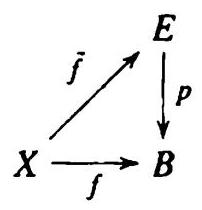
\includegraphics[width=0.2\textwidth]{images/54.0.jpg}
\end{center}
\hspace*{3em} 

The existence of \index{lifting@Lifting}liftings when \(p\) is a covering map is an important tool in studying covering spaces and the fundamental group. First, we show that for a covering space, paths can be lifted; then we show that path homotopies can be lifted as well. First, an example:

\begin{centeredblock}
\begin{example}
	Consider the covering \(p\mathbb{R} \rightarrow  {S}^{1}\) of Theorem 53.1. The path \(f\) . \([  {0,1}]   \rightarrow  {S}^{1}\) beginning at \({b}_{0} = ( {1,0})\) given by \(f( s)  = ( {\cos {\pi s},\sin {\pi s}})\) lifts to the path \(\bar{f}( s)  = s/2\) beginning at 0 and ending at \(\frac{1}{2}\) . The path \(g( s)  = ( {\cos {\pi s}, - \sin {\pi s}})\) lifts to the path \(\bar{g}( s)  =  - s/2\) beginning at 0 and ending at \(- \frac{1}{2}\) The path \(h( s)  = ( {\cos {4\pi s},\sin {4\pi s}})\) lifts to the path \(\bar{h}( s)  = {2s}\) beginning at 0 and ending at 2 . Intuitively, \(h\) wraps the interval \([  {0,1}]\) around the circle twice; this is reflected in the fact that the lifted path \(\bar{h}\) begins at zero and ends at the number 2 These paths are pictured in Figure 541.

\begin{center}
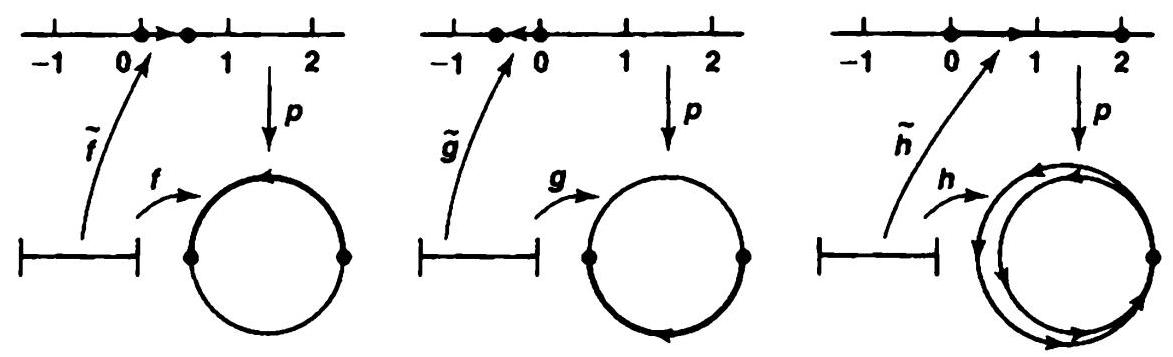
\includegraphics[width=1.0\textwidth]{images/54.1.jpg}
\end{center}
\hspace*{3em} 

Figure 54.1

\begin{lemma}
	Let \(p : E \rightarrow  B\) be a covering map, let \(p( {e}_{0})  = {b}_{0}\) . Any path \(f.[  {0,1}]   \rightarrow  B\) beginning at \({b}_{0}\) has a unique lifting to a path \(\bar{f}\) in \(E\) beginning at \({e}_{0}\) .
\end{lemma}

\begin{proof}
	Cover \(B\) by open sets \(U\) each of which is evenly covered by \(p\) . Find a subdivision of \([  {0,1}]\) , say \({s}_{0},\ldots ,{s}_{n}\) , such that for each \(i\) the set \(f( [  {{s}_{i},{s}_{i + 1}}]  )\) lies in such an open set \(U\) . (Here we use the Lebesgue number lemma.) We define the lifting \(\bar{f}\) step by step.
First, define \(\bar{f}( 0)  = {e}_{0}\) . Then, supposing \(\bar{f}( s)\) is defined for \(0 \leq  s \leq  {s}_{i}\) , we define \(\widetilde{f}\) on \([  {{s}_{i},{s}_{i + 1}}]\) as follows: The set \(f( [  {{s}_{i},{s}_{i + 1}}]  )\) lies in some open set \(U\) that is evenly covered by \(p\) Let \(\{  {V}_{\alpha }]\) be a partition of \({p}^{-1}( U)\) into slices; each set \({V}_{\alpha }\) is mapped homeomorphically onto \(U\) by \(p\) . Now \(\widetilde{f}( {s}_{i})\) lies in one of these sets, say in \({V}_{0}\) . Define \(\bar{f}( s)\) for \(s \in  [  {{s}_{i},{s}_{i + 1}}]\) by the equation

\[
\bar{f}( s)  = {( p \mid  {V}_{0}) }^{-1}( {f( s) }) .
\]

Because \(p \mid  {V}_{0} : {V}_{0} \rightarrow  U\) is a homeomorphism, \(\widetilde{f}\) will be continuous on \([  {{s}_{i},{s}_{i + 1}}]\) .

Continuing in this way, we define \(\widetilde{f}\) on all of \([  {0,1}]\) . Continuity of \(\widetilde{f}\) follows from the pasting lemma; the fact that \(p \circ  \bar{f} = f\) is immediate from the definition of \(\bar{f}\) .

The uniqueness of \(\bar{f}\) is also proved step by step. Suppose that \(\bar{\bar{f}}\) is another lifting of \(f\) beginning at \({e}_{0}\) . Then \(\widetilde{\widetilde{f}}( 0)  = {e}_{0} = \bar{f}( 0)\) . Suppose that \(\overline{\widetilde{f}}( s)  = \widetilde{f}( s)\) for all \(s\) such that \(0 \leq  s \leq  {s}_{i}\) . Let \({V}_{0}\) be as in the preceding paragraph; then for \(s \in  [  {{s}_{i},{s}_{t + 1}}]\) , \(\widetilde{f}( s)\) is defined as \({( p \mid  {V}_{0}) }^{-1}( {f( s) })\) . What can \(\overline{\bar{f}}( s)\) equal? Since \(\overline{\bar{f}}\) is a lifting of \(f\) , it must carry the interval \([  {{s}_{i},{s}_{i + 1}}]\) into the set \({p}^{-1}( U)  = \bigcup {V}_{\alpha }\) . The slices \({V}_{\alpha }\) are open and disjoint; because the set \(\widetilde{\widetilde{f}}( [  {{s}_{i},{s}_{i + 1}}]  )\) is connected, it must lie entirely in one of the sets \({V}_{\alpha }\) . Because \(\widetilde{\bar{f}}( {s}_{i})  = \widetilde{f}( {s}_{i})\) , which is in \({V}_{0},\bar{\bar{f}}\) must carry all of \([  {{s}_{i},{s}_{i + 1}}]\) into the set \({V}_{0}\) . Thus, for \(s\) in \([  {{s}_{i},{s}_{i + 1}}]  ,\widetilde{\bar{f}}( s)\) must equal some point \(y\) of \({V}_{0}\) lying in \({p}^{-1}( {f( s) })\) . But there is only one such point \(y\) , namely, \({( p \mid  {V}_{0}) }^{-1}( {f( s) })\) . Hence \(\widetilde{\widetilde{f}}( s)  = \widetilde{f}( s)\) for \(s \in  [  {{s}_{i},{s}_{i + 1}}]\)
\end{proof}
\begin{lemma}
	Let \(p : E \rightarrow  B\) be a covering map; let \(p( {e}_{0})  = {b}_{0}\) . Let the map \(F : I \times  I \rightarrow  B\) be continuous, with \(F( {0,0})  = {b}_{0}\) . There is a unique lifting of \(F\) to a continuous map

\[
\widetilde{F} : I \times  I \rightarrow  E
\]

such that \(\bar{F}( {0,0})  = {e}_{0}\) . If \(F\) is a path homotopy, then \(\widetilde{F}\) is a path homotopy.
\end{lemma}

\begin{proof}
	Given \(F\) , we first define \(\bar{F}( {0,0})  = {e}_{0}\) . Next, we use the preceding lemma to extend \(\bar{F}\) to the left-hand edge \(0 \times  I\) and the bottom edge \(I \times  0\) of \(I \times  I\) . Then we extend \(\bar{F}\) to all of \(I \times  I\) as follows:
Choose subdivisions

\[
{s}_{0} < {s}_{1} < \cdots  < {s}_{m}
\]

\[
{t}_{0} < {t}_{1} < \cdots  < {t}_{n}
\]

of \(I\) fine enough that each rectangle

\[
{I}_{i} \times  {J}_{j} = [  {{s}_{i - 1},{s}_{i}}]   \times  [  {{t}_{j - 1},{t}_{j}}\}
\]

is mapped by \(F\) into an open set of \(B\) that is evenly covered by \(p\) . (Use the Lebesgue number lemma.) We define the lifting \(\widetilde{F}\) step by step, beginning with the rectangle \({I}_{1} \times  {J}_{1}\) , continuing with the other rectangles \({I}_{t} \times  {J}_{1}\) in the ``bottom row,'' then with the rectangles \({I}_{i} \times  {J}_{2}\) in the next row, and so on.

In general, given \({i}_{0}\) and \({j}_{0}\) , assume that \(\widetilde{F}\) is defined on the set \(A\) which is the union of \(0 \times  I\) and \(I \times  0\) and all the rectangles ``previous'' to \({I}_{{i}_{0}} \times  {J}_{J0}\) (those rectangles \({I}_{i} \times  {J}_{j}\) for which \(j < {j}_{0}\) and those for which \(j = {j}_{0}\) and \(i < {i}_{0}\) ). Assume also that \(\bar{F}\) is a continuous lifting of \(F \mid  A\) . We define \(\bar{F}\) on \({I}_{{i}_{0}} \times  {J}_{{j}_{0}}\) . Choose an open set \(U\) of \(B\) that is evenly covered by \(p\) and contains the set \(F( {{I}_{{t}_{0}} \times  {J}_{{j}_{0}}})\) . Let \(\{  {V}_{\alpha }\}\) be a partition of \({p}^{-1}( U)\) into slices; each set \({V}_{\alpha }\) is mapped homeomorphically onto \(U\) by \(p\) . Now \(\bar{F}\) is already defined on the set \(C = A \cap  ( {{I}_{{i}_{0}} \times  {J}_{{j}_{0}}})\) . This set is the union of the left and bottom edges of the rectangle \({I}_{{i}_{0}} \times  {J}_{{j}_{0}}\) , so it is connected. Therefore, \(\bar{F}( C)\) is connected and must lie entirely within one of the sets \({V}_{\alpha }\) . Suppose it lies in \({V}_{0}\) Then, the situation is as pictured in Figure 54.2.

\begin{center}
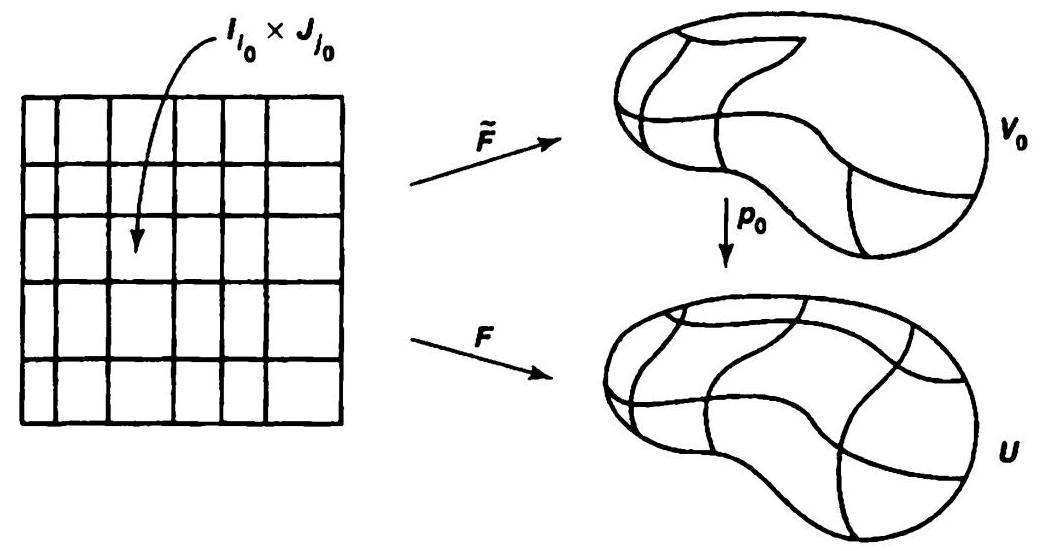
\includegraphics[width=0.9\textwidth]{images/54.2.jpg}
\end{center}
\hspace*{3em} 

Figure 54.2

Let \({p}_{0} : {V}_{0} \rightarrow  U\) denote the restriction of \(p\) to \({V}_{0}\) . Since \(\bar{F}\) is a lifting of \(F \mid  A\) , we know that for \(x \in  C\) ,

\[
{p}_{0}( {\widetilde{F}( x) })  = p( {\bar{F}( x) })  = F( x) ,
\]

so that \(\widetilde{F}( x)  = {p}_{0}^{-1}( {F( x) })\) . Hence we may extend \(\widetilde{F}\) by defining

\[
\widetilde{F}( x)  = {p}_{0}^{-1}( {F( x) })
\]

for \(x \in  {I}_{{i}_{0}} \times  {J}_{{j}_{0}}\) . The extended map will be continuous by the pasting lemma.

Continuing in this way, we define \(\widetilde{F}\) on all of \({I}^{2}\) .

To check uniqueness, note that at each step of the construction of \(\bar{F}\) , as we extend \(\widetilde{F}\) first to the bottom and left edges of \({I}^{2}\) , and then to the rectangles \({I}_{i} \times  {J}_{j}\) , one by one, there is only one way to extend \(\bar{F}\) continuously. Thus, once the value of \(\bar{F}\) at (0,0)is specified, \(\bar{F}\) is completely determined.

Now suppose that \(F\) is a path homotopy. We wish to show that \(\widetilde{F}\) is a path homotopy. The map \(F\) carries the entire left edge \(0 \times  I\) of \({I}^{2}\) into a single point \({b}_{0}\) of \(B\) . Because \(\widetilde{F}\) is a lifting of \(F\) , it carries this edge into the set \({p}^{-1}( {b}_{0})\) . But this set has the discrete topology as a subspace of \(E\) . Since \(0 \times  I\) is connected and \(\widetilde{F}\) is continuous, \(\bar{F}( {0 \times  I})\) is connected and thus must equal a one-point set. Similarly, \(\bar{F}( {1 \times  I})\) must be a one-point set. Thus \(\bar{F}\) is a path homotopy.
\end{proof}
\begin{theorem}
	Let \(p : E \rightarrow  B\) be a covering map; let \(p( {e}_{0})  = {b}_{0}\) . Let \(f\) and \(g\) be two paths in \(B\) from \({b}_{0}\) to \({b}_{1}\) , let \(\widetilde{f}\) and \(\widetilde{g}\) be their respective liftings to paths in \(E\) beginning at \({e}_{0}\) . If \(f\) and \(g\) are path homotopic, then \(\widetilde{f}\) and \(\widetilde{g}\) end at the same point of \(E\) and are path homotopic.
\end{theorem}
\begin{proof}
	Let \(F : I \times  I \rightarrow  B\) be the path homotopy between \(f\) and \(g\) . Then \(F( {0,0})  =\)  \({b}_{0}\) Let \(\bar{F} : I \times  I \rightarrow  E\) be the lifting of \(F\) to \(E\) such that \(\bar{F}( {0,0})  = {e}_{0}\) . By the preceding lemma, \(\bar{F}\) is a path homotopy, so that \(\bar{F}( {0 \times  I})  = \{  {e}_{0}]\) and \(\bar{F}( {1 \times  I})\) is a one-point set \(\{  {e}_{1}]\)

The restriction \(\bar{F} \mid  I \times  0\) of \(\bar{F}\) to the bottom edge of \(I \times  I\) is a path on \(E\) beginning at \({e}_{0}\) that is a lifting of \(F \mid  I \times  0\) . By uniqueness of path liftings, we must have \(\bar{F}( {s,0})  =\)  \(\widetilde{f}( s)\) . Similarly, \(\bar{F} \mid  I \times  1\) is a path on \(E\) that is a lifting of \(F \mid  I \times  1\) , and it begins at \({e}_{0}\) because \(\bar{F}( {0 \times  I})  = \{  {e}_{0}]\) . By uniqueness of path liftings, \(\bar{F}( {s,1})  = \widetilde{g}( s)\) Therefore, both \(\bar{f}\) and \(\bar{g}\) end at \({e}_{1}\) , and \(\bar{F}\) is a path homotopy between them.
\end{proof}

\begin{definition}
	Let \(p : E \rightarrow  B\) be a covering map; let \({b}_{0} \in  B\) Choose \({e}_{0}\) so that \(p( {e}_{0})  = {b}_{0}\) . Given an element \([  f]\) of \({\pi }_{1}( {B,{b}_{0}})\) , let \(\bar{f}\) be the lifting of \(f\) to a path in \(E\) that begins at \({e}_{0}\) . Let \(\phi ( [  f]  )\) denote the end point \(\widetilde{f}( 1)\) of \(\widetilde{f}\) . Then \(\phi\) is a well-defined set map

\[
\phi  : {\pi }_{1}( {B,{b}_{0}})  \rightarrow  {p}^{-1}( {b}_{0}) .
\]

We call \(\phi\) the \index{Lifting correspondence} derived from the covering map \(p\) . It depends of course on the choice of the point \({e}_{0}\) .
\end{definition}

\begin{theorem}
	Let \(p : E \rightarrow  B\) be a covering map; let \(p( {e}_{0})  = {b}_{0}\) . If \(E\) is path connected, then the \index{lifting correspondence@Lifting correspondence}lifting correspondence

\[
\phi  : {\pi }_{1}( {B,{b}_{0}})  \rightarrow  {p}^{-1}( {b}_{0})
\]

is surjective. If \(E\) is simply connected, it is bijective.
\end{theorem}

\begin{proof}
	If \(E\) is path connected, then, given \({e}_{1} \in  {p}^{-1}( {b}_{0})\) , there is a path \(\bar{f}\) in \(E\) from \({e}_{0}\) to \({e}_{1}\) . Then \(f = p \circ  \widetilde{f}\) is a loop in \(B\) at \({b}_{0}\) , and \(\phi ( [  f]  )  = {e}_{1}\) by definition
Suppose \(E\) is simply connected. Let \([  f]\) and \([  g]\) be two elements of \({\pi }_{1}( {B,{b}_{0}})\) such that \(\phi ( [  f]  )  = \phi ( [  g]  )\) . Let \(\bar{f}\) and \(\bar{g}\) be the liftings of \(f\) and \(g\) , respectively, to paths in \(E\) that begin at \({e}_{0}\) , then \(\widetilde{f}( 1)  = \widetilde{g}( 1)\) . Since \(E\) is simply connected, there is a path homotopy \(\widetilde{F}\) in \(E\) between \(\widetilde{f}\) and \(\bar{g}\) . Then \(p \circ  \widetilde{F}\) is a path homotopy in \(B\) between \(f\) and \(g\)
\end{proof}
\begin{theorem}
	The \index{Fundamental group!of \({S}^{1}\)}fundamental group of \({S}^{1}\) is isomorphic to the additive group of integers.
\end{theorem}

\begin{proof}
	Let \(p : \mathbb{R} \rightarrow  {S}^{1}\) be the covering map of Theorem 53.1, let \({e}_{0} = 0\) , and let \({b}_{0} = p( {e}_{0})\) . Then \({p}^{-1}( {b}_{0})\) is the set \(\mathbb{Z}\) of integers. Since \(\mathbb{R}\) is simply connected, the lifting correspondence
\[
\phi  : {\pi }_{1}( {{S}^{1},{b}_{0}})  \rightarrow  \mathbb{Z}
\]

is bijective. We show that \(\phi\) is a homomorphism, and the theorem is proved.

Given \([  f]\) and \([  g]\) in \({\pi }_{1}( {B,{b}_{0}})\) , let \(\widetilde{f}\) and \(\widetilde{g}\) be their respective liftings to paths on \(\mathbb{R}\) beginning at 0 . Let \(n = \widetilde{f}( 1)\) and \(m = \widetilde{g}( 1)\) ; then \(\phi ( [  f]  )  = n\) and \(\phi ( [  g]  )  = m\) , by definition. Let \(\widetilde{\widetilde{g}}\) be the path

\[
\widetilde{\bar{g}}( s)  = n + \widetilde{g}( s)
\]

on \(\mathbb{R}\) . Because \(p( {n + x})  = p( x)\) for all \(x \in  \mathbb{R}\) , the path \(\widetilde{g}\) is a lifting of \(g\) ; it begins at \(n\) . Then the product \(\widetilde{f} * \overline{\widetilde{g}}\) is defined, and it is the lifting of \(f * g\) that begins at 0, as you can check. The end point of this path is \(\widetilde{\widetilde{g}}( 1)  = n + m\) . Then by definition,

\[
\phi ( {[  f]   * [  g]  })  = n + m = \phi ( [  f]  )  + \phi ( [  g]  ) .
\]
\end{proof}
\begin{definition}
	Let \(G\) be a group; let \(x\) be an element of \(G\) . We denote the inverse of \(x\) by \({x}^{-1}\) . The symbol \({x}^{n}\) denotes the \(n\) -fold product of \(x\) with itself, \({x}^{-n}\) denotes the \(n\) -fold product of \({x}^{-1}\) with itself, and \({x}^{0}\) denotes the identity element of \(G\) . If the set of all elements of the form \({x}^{m}\) , for \(m \in  \mathbb{Z}\) , equals \(G\) , then \(G\) is said to be a \index{Cyclic group}, and \(x\) is said to be a \index{generator of cyclic group@Generator of cyclic group} generator of \(G\) .
\end{definition}

The cardinality of a group is also called the \index{order of a group@Order of a group} order of the group. A group is cyclic of infinite order if and only if it is isomorphic to the additive group of integers; it is cyclic of order \(k\) if and only if it is isomorphic to the group \(\mathbb{Z}/k\) of integers modulo \(k\) . The preceding theorem implies that the fundamental group of the circle is infinite cyclic.

Note that if \(x\) is a generator of the infinite cyclic group \(G\) , and if \(y\) is an element of the arbitrary group \(H\) , then there is a unique homomorphism \(h\) of \(G\) into \(H\) such that \(h( x)  = y\) ; it is defined by setting \(h( {x}^{n})  = {y}^{n}\) for all \(n\) .

For later use, in §65 and in Chapters 13 and 14, we prove here a strengthened version of Theorem 54.4.

-Theorem 54.6. Let \(p : E \rightarrow  B\) be a covering map; let \(p( {e}_{0})  = {b}_{0}\) .

(a) The homomorphism \({p}_{ * } : {\pi }_{1}( {E,{e}_{0}})  \rightarrow  {\pi }_{1}( {B,{b}_{0}})\) is a \index{monomorphism@Monomorphism}monomorphism.

(b) Let \(H = {p}_{ * }( {{\pi }_{1}( {E,{e}_{0}}) })\) . The lifting correspondence \(\phi\) induces an injective map

\[
\Phi  : {\pi }_{1}( {B,{b}_{0}}) /H \rightarrow  {p}^{-1}( {b}_{0})
\]

of the collection of right cosets of \(H\) into \({p}^{-1}( {b}_{0})\) , which is bijective if \(E\) is path connected.

(c) If \(f\) is a loop in \(B\) based at \({b}_{0}\) , then \([  f]   \in  H\) if and only if \(f\) lifts to a loop in \(E\) based at \({e}_{0}\) .

\begin{proof}
	(a) Suppose \(\widetilde{h}\) is a loop in \(E\) at \({e}_{0}\) , and \({p}_{ * }( [  \widetilde{h}]  )\) is the identity element. Let \(F\) be a path homotopy between \(p \circ  \widetilde{h}\) and the constant loop. If \(\widetilde{F}\) is the lifting of \(F\) to \(E\) such that \(\widetilde{F}( {0,0})  = {e}_{0}\) , then \(\bar{F}\) is a path homotopy between \(\bar{h}\) and the constant loop at \({e}_{0}\) .
(b) Given loops \(f\) and \(g\) in \(B\) , let \(\bar{f}\) and \(\bar{g}\) be liftings of them to \(E\) that begin at \({e}_{0}\) . Then \(\phi ( [  f]  )  = \bar{f}( 1)\) and \(\phi ( [  g]  )  = \bar{g}( 1)\) . We show that \(\phi ( [  f]  )  = \phi ( [  g]  )\) if and only if \([  f]   \in  H * [  g]\) .

First, suppose that \([  f]   \in  H * [  g]\) . Then \([  f]   = [  {h * g}]\) , where \(h = p \circ  \bar{h}\) for some loop \(\widetilde{h}\) in \(E\) based at \({e}_{0}\) . Now the product \(\bar{h} * \widetilde{g}\) is defined, and it is a lifting of \(h * g\) . Because \([  f]   = [  {h * g}]\) , the liftings \(\bar{f}\) and \(\bar{h} * \widetilde{g}\) , which begin at \({e}_{0}\) , must end at the same point of \(E\) . Then \(\bar{f}\) and \(\widetilde{g}\) end at the same point of \(E\) , so that \(\phi ( [  f]  )  = \phi ( [  g]  )\) . See Figure 54.3.

\begin{center}
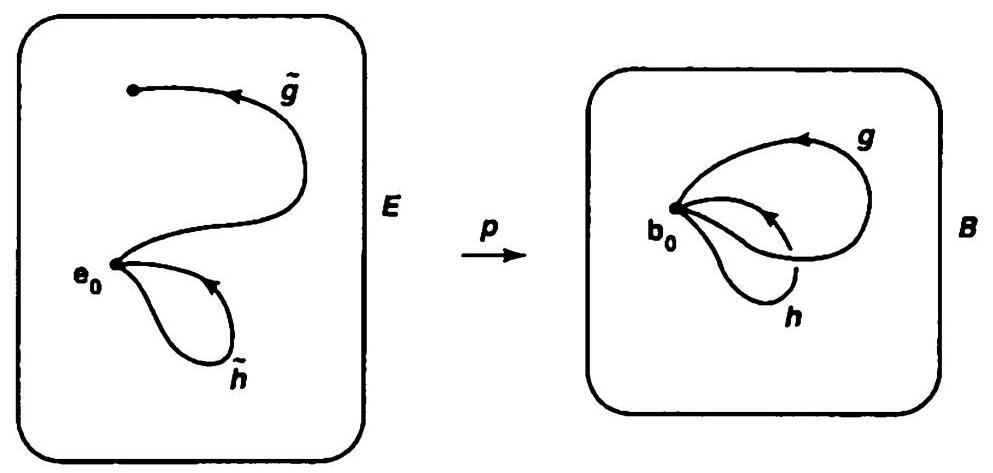
\includegraphics[width=0.9\textwidth]{images/54.3.jpg}
\end{center}
\hspace*{3em} 

Figure 54.3

Now suppose that \(\phi ( [  f]  )  = \phi ( [  g]  )\) . Then \(\bar{f}\) and \(\widetilde{g}\) end at the same point of \(E\) . The product of \(\widetilde{f}\) and the reverse of \(\widetilde{g}\) is defined, and it is a loop \(\widetilde{h}\) in \(E\) based at \({e}_{0}\) . By direct computation, \([  {\widetilde{h} * \widetilde{g}}]   = [  \bar{f}]\) . If \(\bar{F}\) is a path homotopy in \(E\) between the loops \(\widetilde{h} * \widetilde{g}\) and \(\widetilde{f}\) , then \(p \circ  \bar{F}\) is a path homotopy in \(B\) between \(h * g\) and \(f\) , where \(h = p \circ  \widetilde{h}\) . Thus \([  f]   \in  H * [  g]\) , as desired.

If \(E\) is path connected, then \(\phi\) is surjective, so that \(\Phi\) is surjective as well.

(c) Injectivity of \(\Phi\) means that \(\phi ( [  f]  )  = \phi ( [  g]  )\) if and only if \([  f]   \in  H * [  g]\) . Applying this result in the case where \(g\) is the constant loop, we see that \(\phi ( [  f]  )  = {e}_{0}\) if and only if \([  f]   \in  H\) . But \(\phi ( [  f]  )  = {e}_{0}\) precisely when the lift of \(f\) that begins at \({e}_{0}\) also ends at \({e}_{0}\) .
\end{proof}
\section*{Exercises}
\begin{enumerate}[itemsep=0.4em, parsep=0pt, topsep=0pt, partopsep=0pt, leftmargin=*, label=\arabic*., ref=\arabic*]
\item What goes wrong with the ``path-lifting lemma'' (Lemma 54.1) for the local homeomorphism of Example 2 of §53?
\item In defining the map \(\bar{F}\) in the proof of Lemma 54.2, why were we so careful about the order in which we considered the small rectangles?
\item Let \(p : E \rightarrow  B\) be a covering map. Let \(\alpha\) and \(\beta\) be paths in \(B\) with \(\alpha ( 1)  = \beta ( 0)\) ; let \(\bar{\alpha }\) and \(\bar{\beta }\) be liftings of them such that \(\widetilde{\alpha }( 1)  = \widetilde{\beta }( 0)\) . Show that \(\bar{\alpha } * \bar{\beta }\) is a lifting of \(\alpha  * \beta\) .
\item Consider the covering map \(p : \mathbb{R} \times  {\mathbb{R}}_{ + } \rightarrow  {\mathbb{R}}^{2} - 0\) of Example 6 of \(§{53}\) . Find liftings of the paths \[ f( t)  = ( {2 - t,0}) , \] \[ g( t)  = ( {( {1 + t}) \cos {2\pi t},( {1 + t}) \sin {2\pi t}}) \] \[ h( t)  = f * g. \] Sketch these paths and their liftings.
\item Consider the covering map \(p \times  p : \mathbb{R} \times  \mathbb{R} \rightarrow  {S}^{1} \times  {S}^{1}\) of Example 4 of \(§{53}\) . Consider the path \[ f( t)  = ( {\cos {2\pi t},\sin {2\pi t}})  \times  ( {\cos {4\pi t},\sin {4\pi t}}) \] in \({S}^{1} \times  {S}^{1}\) . Sketch what \(f\) looks like when \({S}^{1} \times  {S}^{1}\) is identified with the doughnut surface \(D\) . Find a lifting \(\bar{f}\) of \(f\) to \(\mathbb{R} \times  \mathbb{R}\) , and sketch it.
\item Consider the maps \(g,h : {S}^{1} \rightarrow  {S}^{1}\) given \(g( z)  = {z}^{n}\) and \(h( z)  = 1/{z}^{n}\) . (Here we represent \({S}^{1}\) as the set of complex numbers \(z\) of absolute value 1 .) Compute the induced homomorphisms \({g}_{ * },{h}_{ * }\) of the infinite \index{cyclic group@Cyclic group}cyclic group \({\pi }_{1}( {{S}^{1},{b}_{0}})\) into itself. [Hint: Recall the equation \({( \cos \theta  + i\sin \theta ) }^{n} = \cos {n\theta } + i\sin {n\theta }\) .]
\item Generalize the proof of Theorem 54.5 to show that the fundamental group of the torus is isomorphic to the group \(\mathbb{Z} \times  \mathbb{Z}\) .
\item Let \(p : E \rightarrow  B\) be a covering map, with \(E\) path connected. Show that if \(B\) is simply connected, then \(p\) is a homeomorphism.
\end{enumerate}
\section*{§ 55 Retractions and Fixed Points}

We now prove several classical results of topology that follow from our knowledge of the fundamental group of \({S}^{1}\) .

\begin{definition}
	If \(A \subset  X\) , a retraction of \(X\) onto \(A\) is a continuous map \(r : X \rightarrow  A\) such that \(r \mid  A\) is the identity map of \(A\) . If such a map \(r\) exists, we say that \(A\) is a retract of \(X\) .
\end{definition}

\begin{lemma}
	If \(A\) is a retract of \(X\) , then the homomorphism of fundamental groups induced by inclusion \(j : A \rightarrow  X\) is injective.
\end{lemma}

\begin{proof}
	If \(r : X \rightarrow  A\) is a retraction, then the composite map \(r \circ  j\) equals the identity map of \(A\) . It follows that \({r}_{ * } \circ  {j}_{ * }\) is the identity map of \({\pi }_{1}( {A,a})\) , so that \({j}_{ * }\) must be injective.
\end{proof}
\begin{theorem}[\index{no-retraction theorem@No-retraction theorem}]
	There is no retraction of \({B}^{2}\) onto \({S}^{1}\) .
\end{theorem}

\begin{proof}
	If \({S}^{1}\) were a retract of \({B}^{2}\) , then the homomorphism induced by inclusion \(j : {S}^{1} \rightarrow  {B}^{2}\) would be injective. But the fundamental group of \({S}^{1}\) is nontrivial and the \index{B^n@\({B}^{n}\)!fundamental group}fundamental group of \({B}^{2}\) is trivial.
\end{proof}
\begin{lemma}
	Let \(h : {S}^{1} \rightarrow  X\) be a continuous map Then the following conditions are equivalent:

(I) \(h\) is nulhomotopic.

(2) \(h\) extends to a continuous map \(k : {B}^{2} \rightarrow  X\) .

(3) \({h}_{ * }\) is the \index{trivial homomorphism@Trivial homomorphism}trivial homomorphism of fundamental groups.
\end{lemma}

\begin{proof}
	(1) \(\Rightarrow\) (2). Let \(H : {S}^{1} \times  I \rightarrow  X\) be a homotopy between \(h\) and a constant map. Let \(\pi  : {S}^{1} \times  I \rightarrow  {B}^{2}\) be the map
\[
\pi ( {x,t})  = ( {1 - t}) x.
\]

Then \(\pi\) is continuous, closed and surjective, so it is a quotient map; it collapses \({S}^{1} \times  1\) to the point0and is otherwise injective. Because \(H\) is constant on \({S}^{1} \times  1\) , it induces, via the quotient map \(\pi\) , a continuous map \(k : {B}^{2} \rightarrow  X\) that is an extension of \(h\) . See Figure 55.1.

\begin{center}
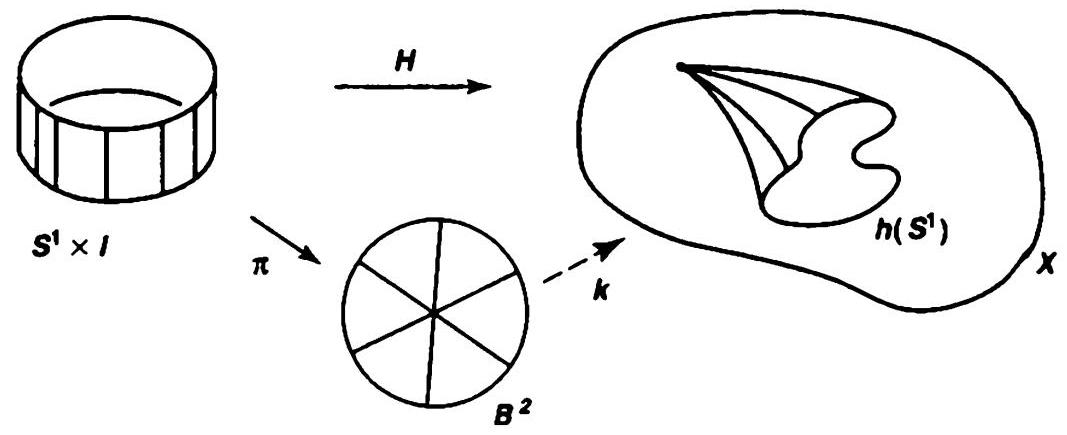
\includegraphics[width=0.9\textwidth]{images/55.1.jpg}
\end{center}
\hspace*{3em} 

Figure 55.1

\(( 2)  \Rightarrow  ( 3)\) . If \(j : {S}^{1} \rightarrow  {B}^{2}\) is the inclusion map, then \(h\) equals the composite \(k \circ  j\) . Hence \({h}_{ * } = {k}_{ * } \circ  {j}_{ * }\) . But

\[
{j}_{ * } : {\pi }_{1}( {{S}^{1},{b}_{0}})  \rightarrow  {\pi }_{1}( {{B}^{2},{b}_{0}})
\]

is trivial because the fundamental group of \({B}^{2}\) is trivial. Therefore \({h}_{ * }\) is trivial.

\(( 3)  \Rightarrow  ( 1)\) . Let \(p : \mathbb{R} \rightarrow  {S}^{1}\) be the standard covering map, and let \({p}_{0} : I \rightarrow  {S}^{1}\) be its restriction to the unit interval. Then \([  {p}_{0}]\) generates \({\pi }_{1}( {{S}^{1},{b}_{0}})\) because \({p}_{0}\) is a loop in \({S}^{1}\) whose lift to \(\mathbb{R}\) begins at 0 and ends at 1 .

Let \({x}_{0} = h( {b}_{0})\) . Because \({h}_{ * }\) is trivial, the loop \(f = h \circ  {p}_{0}\) represents the identity element of \({\pi }_{1}( {X,{x}_{0}})\) . Therefore, there is a path homotopy \(F\) in \(X\) between \(f\) and the constant path at \({x}_{0}\) . The map \({p}_{0} \times  \mathrm{{id}} \cdot  I \times  I \rightarrow  {S}^{1} \times  I\) is a quotient map, being continuous, closed, and surjective; it maps \(0 \times  t\) and \(1 \times  t\) to \({b}_{0} \times  t\) for each \(t\) , but is otherwise injective. The path homotopy \(F\) maps \(0 \times  I\) and \(1 \times  I\) and \(I \times  1\) to the point \({x}_{0}\) of \(X\) , so it induces a continuous map \(H : {S}^{1} \times  I \rightarrow  X\) that is a homotopy between \(h\) and a constant map. See Figure 55.2.

\begin{center}
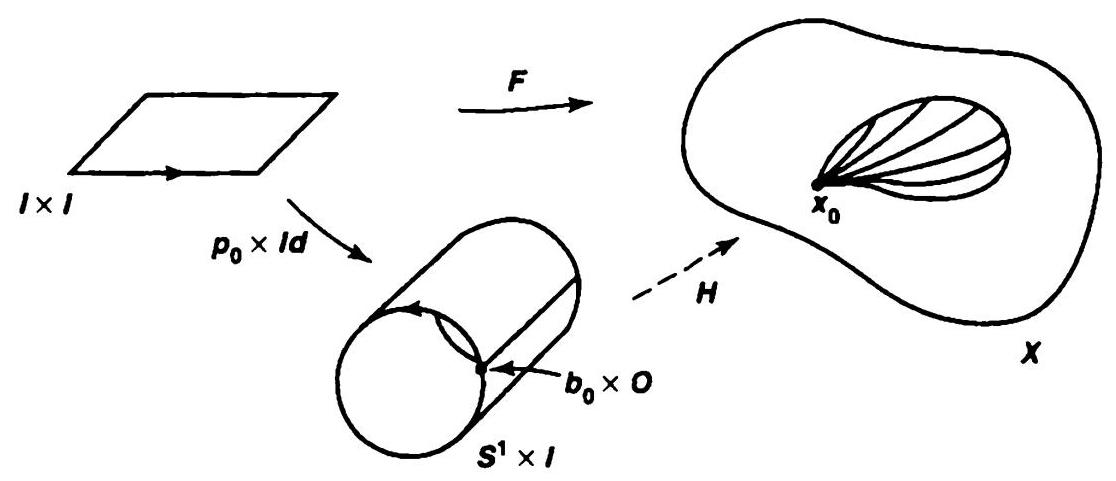
\includegraphics[width=1.0\textwidth]{images/55.2.jpg}
\end{center}
\hspace*{3em} 

Figure 55.2
\end{proof}
\begin{corollary}
	The inclusion map \(j \cdot  {S}^{1} \rightarrow  {\mathbb{R}}^{2} - 0\) is not nulhomotopic. The identity map \(i : {S}^{1} \rightarrow  {S}^{1}\) is not nulhomotopic.
\end{corollary}

\begin{proof}
	There is a retraction of \({\mathbb{R}}^{2} - 0\) onto \({S}^{1}\) given by the equation \(r( x)  = x/\parallel x\parallel\) . Therefore, \({j}_{ * }\) is injective, and hence nontrivial. Similarly, \({i}_{ * }\) is the identity homomorphism, and hence nontrivial.
\end{proof}
\begin{theorem}
	Given a nonvanishing \index{Vector field} on \({B}^{2}\) , there exists a point of \({S}^{1}\) where the \index{vector field@Vector field}vector field points directly inward and a point of \({S}^{1}\) where it points directly outward.
\end{theorem}

\begin{proof}
	A vector field on \({B}^{2}\) is an ordered pair \(( {x,v( x) })\) , where \(x\) is in \({B}^{2}\) and \(v\) is a continuous map of \({B}^{2}\) into \({\mathbb{R}}^{2}\) . In calculus, one often uses the notation
\[
\mathbf{v}( x)  = {v}_{1}( x) \mathbf{i} + {v}_{2}( x) \mathbf{j}
\]

for the function \(v\) , where \(\mathrm{i}\) and \(\mathrm{j}\) are the standard unit basis vectors in \({\mathbb{R}}^{2}\) . But we shall stick with simple functional notation. To say that a vector field is nonvanishing means that \(v( x)  \neq  \mathbf{0}\) for every \(x\) ; in such a case \(v\) actually maps \({B}^{2}\) into \({\mathbb{R}}^{2} - \mathbf{0}\) .

We suppose first that \(v( x)\) does not point directly inward at any point \(x\) of \({S}^{1}\) and derive a contradiction. Consider the map \(v : {B}^{2} \rightarrow  {\mathbb{R}}^{2} - \mathbf{0}\) ; let \(w\) be its restriction to \({S}^{1}\) . Because the map \(w\) extends to a map of \({B}^{2}\) into \({\mathbb{R}}^{2} - \mathbf{0}\) , it is nulhomotopic.

On the other hand, \(w\) is homotopic to the inclusion map \(j : {S}^{1} \rightarrow  {\mathbb{R}}^{2} - \mathbf{0}\) . Figure 55.3 illustrates the homotopy; one defines it formally by the equation

\[
F( {x,t})  = {tx} + ( {1 - t}) w( x) ,
\]

for \(x \in  {S}^{1}\) . We must show that \(F( {x,t})  \neq  \mathbf{0}\) . Clearly, \(F( {x,t})  \neq  \mathbf{0}\) for \(t = 0\) and \(t = 1\) . If \(F( {x,t})  = 0\) for some \(t\) with \(0 < t < 1\) , then \({tx} + ( {1 - t}) w( x)  = 0\) , so that \(w( x)\) equals a negative scalar multiple of \(x\) . But this means that \(w( x)\) points directly inward at \(x\) ! Hence \(F\) maps \({S}^{1} \times  I\) into \({\mathbb{R}}^{2} - \mathbf{0}\) , as desired.

It follows that \(j\) is nulhomotopic, contradicting the preceding corollary.

To show that \(v\) points directly outward at some point of \({S}^{1}\) , we apply the result just proved to the vector field \(( {x, - v( x) })\) .

\begin{center}
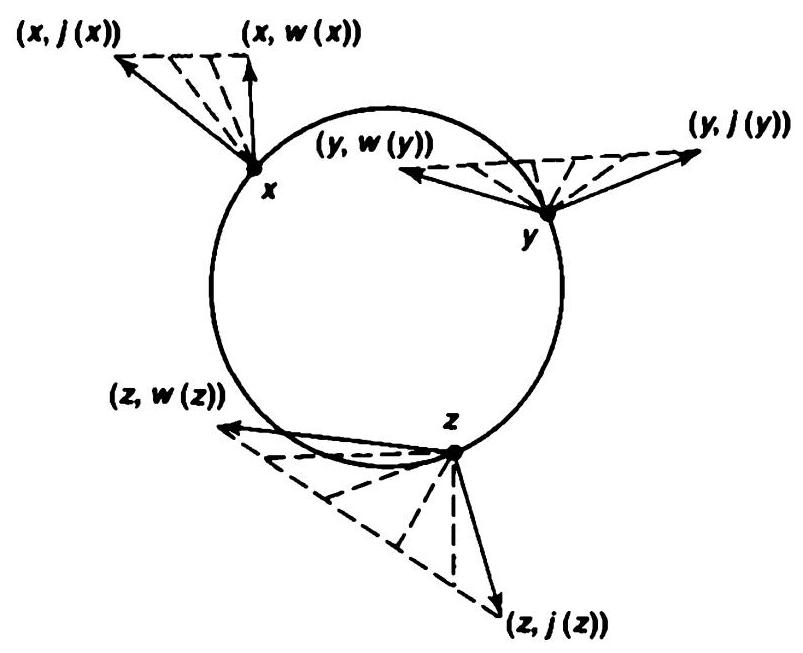
\includegraphics[width=0.7\textwidth]{images/55.3.jpg}
\end{center}
\hspace*{3em} 

Figure 55.3

We have already seen that every continuous map \(f : [  {0,1}]   \rightarrow  [  {0,1}]\) has a fixed point (see Exercise 3 of \(§{24}\) ). The same is true for the ball \({B}^{2}\) , although the proof is deeper:
\end{proof}
\begin{theorem}[\index{brouwer fixed-point theorem@Brouwer fixed-point theorem} for the disc]
	If \(f : {B}^{2} \rightarrow  {B}^{2}\) is continuous, then there exists a point \(x \in  {B}^{2}\) such that \(f( x)  = x\) .
\end{theorem}

\begin{proof}
	We proceed by contradiction. Suppose that \(f( x)  \neq  x\) for every \(x\) in \({B}^{2}\) . Then defining \(v( x)  = f( x)  - x\) gives us a nonvanishing vector field \(( {x,v( x) })\) on \({B}^{2}\) . But the vector field \(v\) cannot point directly outward at any point \(x\) of \({S}^{1}\) , for that would mean
\[
f( x)  - x = {ax}
\]

for some positive real number \(a\) , so that \(f( x)  = ( {1 + a}) x\) would lie outside the unit ball \({B}^{2}\) . We thus arrive at a contradiction.

One might well wonder why fixed-point theorems are of interest in mathematics. It turns out that many problems, such as problems concerning existence of solutions for systems of equations, for instance, can be formulated as fixed-point problems. Here is one example, a classical theorem of \index{frobenius theorem@Frobenius theorem} Frobenius. We assume some knowledge of linear algebra at this point.

*Corollary 55.7. Let \(A\) be a 3 by 3 matrix of positive real numbers. Then \(A\) has a positive real eigenvalue (characteristic value).

Proof. Let \(T : {\mathbb{R}}^{3} \rightarrow  {\mathbb{R}}^{3}\) be the linear transformation whose matrix (relative to the standard basis for \({\mathbb{R}}^{3}\) ) is \(A\) . Let \(B\) be the intersection of the 2 -sphere \({S}^{2}\) with the first octant

\[
\{  {( {{x}_{1},{x}_{2},{x}_{3}})  \mid  {x}_{1} \geq  0\text{ and }{x}_{2} \geq  0\text{ and }{x}_{3} \geq  0}\}
\]

of \({\mathbb{R}}^{3}\) . It is easy to show that \(B\) is homeomorphic to the ball \({B}^{2}\) , so that the fixed-point theorem holds for continuous maps of \(B\) into itself.

Now if \(x = ( {{x}_{1},{x}_{2},{x}_{3}})\) is in \(B\) , then all the components of \(x\) are nonnegative and at least one is positive. Because all entries of \(A\) are positive, the vector \(T( x)\) is a vector all of whose components are positive. As a result, the map \(x \rightarrow  T( x) /\parallel T( x) \parallel\) is a continuous map of \(B\) to itself, which therefore has a fixed point \({x}_{0}\) . Then

\[
T( {x}_{0})  = \begin{Vmatrix}{T( {x}_{0}) }\end{Vmatrix}{x}_{0},
\]

so that \(T\) (and therefore the matrix \(A\) ) has the positive real eigenvalue \(\begin{Vmatrix}{T( {x}_{0}) }\end{Vmatrix}\) .

Finally, we prove a theorem that implies that the triangular region

\[
T = \{ ( {x,y})  \mid  x \geq  0\text{ and }y \geq  0\text{ and }x + y \leq  1\}
\]

in \({\mathbb{R}}^{2}\) has topological dimension at least 2. (See \(§{50}\) .)

-Theorem 55.8. There is an \(\epsilon  > 0\) such that for every open covering \(\mathcal{A}\) of \(T\) by sets of diameter less than \(\epsilon\) , some point of \(T\) belongs to at least three elements of \(\mathcal{A}\) .

Proof. We use the fact that \(T\) is homeomorphic to \({B}^{2}\) , so that we can apply the results proved in this section to the space \(T\) .

Choose \(\epsilon  > 0\) so that no set of diameter less than \(\epsilon\) intersects all three edges of \(T\) . (In fact, \(\epsilon  = \frac{1}{2}\) will do.) We suppose that \(\mathcal{A} = \{  {{U}_{1},\ldots ,{U}_{n}}\}\) is an open covering of \(T\) by sets of diameter less than \(\epsilon\) , such that no three elements of \(\mathcal{A}\) intersect, and derive a contradiction.

For each \(i = 1,\ldots ,n\) , choose a vertex \({v}_{i}\) of \(T\) as follows: If \({U}_{i}\) intersects two edges of \(T\) , let \({v}_{i}\) be the vertex common to these edges. If \({U}_{i}\) intersects only one edge of \(T\) , let \({v}_{i}\) be one of the end points of this edge. If \({U}_{i}\) intersects no edge of \(T\) , let \({v}_{i}\) be any vertex of \(T\) .

Now let \(\{  {\phi }_{i}\}\) be a partition of unity dominated by \(\{  {{U}_{1},\ldots ,{U}_{n}}\}\) . (See \(§{36}\) .) Define \(k : T \rightarrow  {\mathbb{R}}^{2}\) by the equation

\[
k( x)  = \mathop{\sum }\limits_{{i = 1}}^{n}{\phi }_{i}( x) {v}_{i}
\]

Then \(k\) is continuous. Given a point \(x\) of \(T\) , it lies in at most two elements of \(\mathcal{A}\) ; hence at most two of the numbers \({\phi }_{i}( x)\) are nonzero. Then \(k( x)  = {v}_{i}\) if \(x\) lies in only one open set \({U}_{i}\) , and \(k( x)  = t{v}_{i} + ( {1 - t}) {v}_{j}\) for some \(t\) with \(0 \leq  t \leq  1\) if \(x\) lies in two open sets \({U}_{i}\) and \({U}_{j}\) . In either case, \(k( x)\) belongs to the union of the edges of \(T\) , which is Bd \(T\) . Thus \(k\) maps \(T\) into Bd \(T\) .

Furthermore, \(k\) maps each edge of \(T\) into itself. For if \(x\) belongs to the edge \({vw}\) of \(T\) , any open set \({U}_{i}\) containing \(x\) intersects this edge, so that \({v}_{i}\) must equal either \(v\) or \(w\) . The definition of \(k\) then shows that \(k( x)\) belongs to \({vw}\) .

Let \(h : \operatorname{Bd}T \rightarrow  \operatorname{Bd}T\) be the restriction of \(k\) to \(\operatorname{Bd}T\) . Since \(h\) can be extended to the continuous map \(k\) , it is nulhomotopic. On the other hand, \(h\) is homotopic to the identity map of \(\operatorname{Bd}T\) to itself; indeed, since \(h\) maps each edge of \(T\) into itself, the straight-line homotopy between \(h\) and the identity map of \(\operatorname{Bd}T\) is such a homotopy. But the identity map \(i\) of \(\operatorname{Bd}T\) is not nulhomotopic.
\end{proof}
\section*{Exercises}
\begin{enumerate}[itemsep=0.4em, parsep=0pt, topsep=0pt, partopsep=0pt, leftmargin=*, label=\arabic*., ref=\arabic*]
\item Show that if \(A\) is a retract of \({B}^{2}\) , then every continuous map \(f : A \rightarrow  A\) has a fixed point.
\item Show that if \(h : {S}^{1} \rightarrow  {S}^{1}\) is nulhomotopic, then \(h\) has a fixed point and \(h\) maps some point \(x\) to its \index{antipode@Antipode}antipode \(- x\)
\item Show that if \(A\) is a nonsingular 3 by 3 matrix having nonnegative entries, then \(A\) has a positive real eigenvalue.
\item Suppose that you are given the fact that for each \(n\) , there is no \index{retraction@Retraction}retraction \(r\) : \({B}^{n + 1} \rightarrow  {S}^{n}\) . (This result can be proved using more advanced techniques of algebraic topology.) Prove the following:
  \begin{enumerate}[itemsep=0.2em, parsep=0pt, topsep=0pt, partopsep=0pt, leftmargin=*, label=(\alph*), align=left]
  \item The identity map \(i : {S}^{n} \rightarrow  {S}^{n}\) is not nulhomotopic.
  \item The inclusion map \(j : {S}^{n} \rightarrow  {\mathbb{R}}^{n + 1} - \mathbf{0}\) is not nulhomotopic.
  \item Every nonvanishing vector field on \({B}^{n + 1}\) points directly outward at some point of \({S}^{n}\) , and directly inward at some point of \({S}^{n}\) .
  \item Every continuous map \(f : {B}^{n + 1} \rightarrow  {B}^{n + 1}\) has a fixed point.
  \item Every \(n + 1\) by \(n + 1\) matrix with positive real entries has a positive eigenvalue.
  \item If \(h : {S}^{n} \rightarrow  {S}^{n}\) is nulhomotopic, then \(h\) has a fixed point and \(h\) maps some point \(x\) to its antipode \(- x\) .
  \end{enumerate}
\end{enumerate}
\section*{*§ 56 The Fundamental Theorem of Algebra}

It is a basic fact about the complex numbers that every polynomial equation

\[
{x}^{n} + {a}_{n - 1}{x}^{n - 1} + \cdots  + {a}_{1}x + {a}_{0} = 0
\]

of \index{degree of a map@Degree of a map} degree \(n\) with real or complex coefficients has \(n\) roots (if the roots are counted according to their multiplicities). You probably first were told this fact in high school algebra, although it is doubtful that it was proved for you at that time.

The proof is, in fact, rather hard; the most difficult part is to prove that every polynomial equation of positive degree has at least one root. There are various ways of doing this. One can use only techniques of algebra; this proof is long and arduous. Or one can develop the theory of analytic functions of a complex variable to the point where it becomes a trivial corollary of Liouville's theorem. Or one can prove it as a relatively easy corollary of our computation of the fundamental group of the circle; this we do now.

\begin{theorem}[The fundamental theorem of algebra]
	A polynomial equation

\[
{x}^{n} + {a}_{n - 1}{x}^{n - 1} + \cdots  + {a}_{1}x + {a}_{0} = 0
\]

of degree \(n > 0\) with real or complex coefficients has at least one (real or complex) root.
\end{theorem}

\begin{proof}
	Step 1. Consider the map \(f : {S}^{1} \rightarrow  {S}^{1}\) given by \(f( z)  = {z}^{n}\) , where \(z\) is a complex number. We show that the induced homomorphism \({f}_{ * }\) of fundamental groups is injective.
Let \({p}_{0} : I \rightarrow  {S}^{1}\) be the standard loop in \({S}^{1}\) ,

\[
{p}_{0}( s)  = {e}^{2\pi is} = ( {\cos {2\pi s},\sin {2\pi s}}) .
\]

Its image under \({f}_{ * }\) is the loop

\[
f( {{p}_{0}( s) })  = {( {e}^{2\pi is}) }^{n} = ( {\cos {2\pi ns},\sin {2\pi ns}}) .
\]

This loop lifts to the path \(s \rightarrow  {ns}\) in the covering space \(\mathbb{R}\) . Therefore, the loop \(f \circ  {p}_{0}\) corresponds to the integer \(n\) under the standard isomorphism of \({\pi }_{1}( {{S}^{1},{b}_{0}})\) with the integers, whereas \({p}_{0}\) corresponds to the number 1 . Thus \({f}_{ * }\) is ``multiplication by \(n\) `` in the fundamental group of \({S}^{1}\) , so that in particular, \({f}_{ * }\) is injective.

Step 2. We show that if \(g : {S}^{1} \rightarrow  {\mathbb{R}}^{2} - \mathbf{0}\) is the map \(g( z)  = {z}^{n}\) , then \(g\) is not nulhomotopic.

The map \(g\) equals the map \(f\) of Step 1 followed by the inclusion map \(j : {S}^{1} \rightarrow\)  \({\mathbb{R}}^{2} - \mathbf{0}\) . Now \({f}_{ * }\) is injective, and \({j}_{ * }\) is injective because \({S}^{1}\) is a retract of \({\mathbb{R}}^{2} - \mathbf{0}\) . Therefore, \({g}_{ * } = {j}_{ * } \circ  {f}_{ * }\) is injective. Thus \(g\) cannot be nulhomotopic.

Step 3. Now we prove a special case of the theorem. Given a polynomial equation

\[
{x}^{n} + {a}_{n - 1}{x}^{n - 1} + \cdots  + {a}_{1}x + {a}_{0} = 0,
\]

we assume that

\[
| {a}_{n - 1}|  + \cdots  + | {a}_{1}|  + | {a}_{0}|  < 1
\]

and show that the equation has a root lying in the unit ball \({B}^{2}\) .

Assume it has no such root. Then we can define a map \(k : {B}^{2} \rightarrow  {\mathbb{R}}^{2} - \mathbf{0}\) by the equation

\[
k( z)  = {z}^{n} + {a}_{n - 1}{z}^{n - 1} + \cdots  + {a}_{1}z + {a}_{0}.
\]

Let \(h\) be the restriction of \(k\) to \({S}^{1}\) . Because \(h\) extends to a map of the unit ball into \({\mathbb{R}}^{2} - 0\) , the map \(h\) is nulhomotopic.

On the other hand, we shall define a homotopy \(F\) between \(h\) and the map \(g\) of Step 2: since \(g\) is not nulhomotopic, we have a contradiction. We define \(F : {S}^{1} \times  I \rightarrow\)  \({\mathbb{R}}^{2} - 0\) by the equation

\[
F( {z,t})  = {z}^{n} + t( {{a}_{n - 1}{z}^{n - 1} + \cdots  + {a}_{0}}) .
\]

See Figure 56.1; \(F( {z,t})\) never equals 0 because

\[
| {F( {z,t}) }|  \geq  | {z}^{n}|  - | {t( {{a}_{n - 1}{z}^{n - 1} + \cdots  + {a}_{0}}) }|
\]

\[
\geq  1 - t( {| {{a}_{n - 1}{z}^{n - 1}}|  + \cdots  + | {a}_{0}| })
\]

\[
= 1 - t( {| {a}_{n - 1}|  + \cdots  + | {a}_{0}| })  > 0\text{ . }
\]

\begin{center}
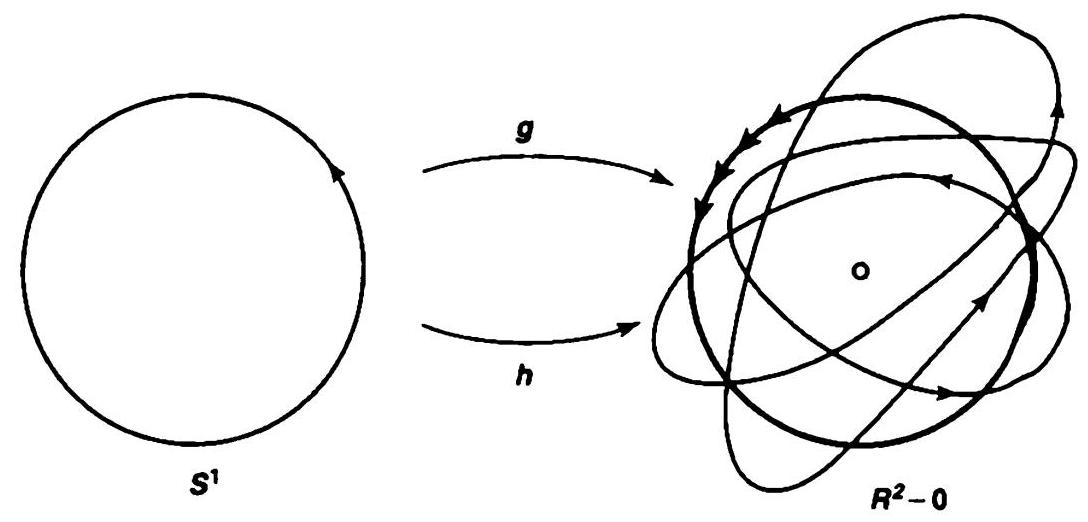
\includegraphics[width=1.0\textwidth]{images/56.1.jpg}
\end{center}
\hspace*{3em} 

Figure 56.1

Step 4. Now we prove the general case. Given a polynomial equation

\[
{x}^{n} + {a}_{n - 1}{x}^{n - 1} + \cdots  + {a}_{1}x + {a}_{0} = 0,
\]

let us choose a real number \(c > 0\) and substitute \(x = {cy}\) . We obtain the equation

\[
{( cy) }^{n} + {a}_{n - 1}{( cy) }^{n - 1} + \cdots  + {a}_{1}( {cy})  + {a}_{0} = 0
\]

or

\[
{y}^{n} + \frac{{a}_{n - 1}}{c}{y}^{n - 1} + \cdots  + \frac{{a}_{1}}{{c}^{n - 1}}y + \frac{{a}_{0}}{{c}^{n}} = 0.
\]

If this equation has the root \(y = {y}_{0}\) , then the original equation has the root \({x}_{0} = c{y}_{0}\) . So we need merely choose \(c\) large enough that

\[
| \frac{{a}_{n - 1}}{c}|  + | \frac{{a}_{n - 2}}{{c}^{2}}|  + \cdots  + | \frac{{a}_{1}}{{c}^{n - 1}}|  + | \frac{{a}_{0}}{{c}^{n}}|  < 1
\]

to reduce the theorem to the special case considered in Step 3.
\end{proof}
\section*{Exercises}
\begin{enumerate}[itemsep=0.4em, parsep=0pt, topsep=0pt, partopsep=0pt, leftmargin=*, label=\arabic*., ref=\arabic*]
\item Given a polynomial equation \[ {x}^{n} + {a}_{n - 1}{x}^{n - 1} + \cdots  + {a}_{1}x + {a}_{0} = 0 \] with real or complex coefficients. Show that if \(| {a}_{n - 1}|  + \cdots  + | {a}_{1}|  + | {a}_{0}|  < 1\) , then all the roots of the equation lie interior to the unit ball \({B}^{2}\) . [Hint: Let \(g( x)  = 1 + {a}_{n - 1}x + \cdots  + {a}_{1}{x}^{n - 1} + {a}_{0}{x}^{n}\) , and show that \(g( x)  \neq  0\) for \(x \in  {B}^{2}\) .]
\item Find a circle about the origin containing all the roots of the polynomial equation \({x}^{7} + {x}^{2} + 1 = 0.\)
\end{enumerate}
\section*{*§ 57 The Borsuk-Ulam Theorem}

\index{borsuk-ulam theorem@Borsuk-Ulam Theorem} Here is a ``brain-teaser'' problem: Suppose you are given a bounded polygonal region \(A\) in the plane \({\mathbb{R}}^{2}\) . No matter what shape \(A\) has, it is easy to show that there exists a straight line that bisects \(A\) , that is, one that cuts the area of \(A\) in half. Simply take the horizontal line \(y = c\) , let \(f( c)\) denote the area of that part of \(A\) that lies beneath this line, note that \(f\) is a continuous function of \(c\) , and use the intermediate-value theorem to find a value of \(c\) for which \(f( c)\) equals exactly half the area of \(A\) .

But now suppose instead that you are given two such regions \({A}_{1}\) and \({A}_{2}\) , you are asked to find a single line that bisects them both. It is not obvious even that there exists such a line. Try to find one for an arbitrary pair \index{Topological dimension!of triangular region}of triangular regions if you have doubts!

In fact, such a line always exists This result is a corollary of a well-known theorem called the \index{borsuk-ulam theorem@Borsuk-Ulam theorem}Borsuk-Ulam theorem, to which we now turn.

\begin{definition}
	If \(x\) is a point of \({S}^{n}\) , then its antipode is the point \(- x\) . A map \(h : {S}^{n} \rightarrow\)  \({S}^{m}\) is said to be \index{antipode-preserving@Antipode-preserving}antipode-preserving if \(h( {-x})  =  - h( x)\) for all \(x \in  {S}^{n}\) .
\end{definition}

\begin{theorem}
	If \(h : {S}^{1} \rightarrow  {S}^{1}\) is continuous and antipode-preserving, then \(h\) is not nulhomotopic.
\end{theorem}

\begin{proof}
	Let \({b}_{0}\) be the point(1,0)of \({S}^{1}\) . Let \(\rho  : {S}^{1} \rightarrow  {S}^{1}\) be a rotation of \({S}^{1}\) that maps \(h( {b}_{0})\) to \({b}_{0}\) . Since \(\rho\) preserves antipodes, so does the composite \(\rho  \circ  h\) . Furthermore, if \(H\) were a homotopy between \(h\) and a constant map, then \(\rho  \circ  H\) would be a homotopy between \(\rho  \circ  h\) and a constant map. Therefore, it suffices to prove the theorem under the additional hypothesis that \(h( {b}_{0})  = {b}_{0}\) .
Step 1. Let \(q : {S}^{1} \rightarrow  {S}^{1}\) be the map \(q( z)  = {z}^{2}\) , where \(z\) is a complex number. Or in real coordinates, \(q( {\cos \theta ,\sin \theta })  = ( {\cos {2\theta },\sin {2\theta }})\) . The map \(q\) is a quotient map, being continuous, closed, and surjective. The inverse image under \(q\) of any point of \({S}^{1}\) consists of two antipodal points \(z\) and \(- z\) of \({S}^{1}\) . Because \(h( {-z})  =  - h( z)\) , one has the equation \(q( {h( {-z}) })  = q( {h( z) })\) . Therefore, because \(q\) is a quotient map, the map \(q \circ  h\) induces a continuous map \(k : {S}^{1} \rightarrow  {S}^{1}\) such that \(k \circ  q = q \circ  h\) . Note that \(q( {b}_{0})  = h( {b}_{0})  = {b}_{0}\) , so that \(k( {b}_{0})  = {b}_{0}\) as well. Also, \(h( {-{b}_{0}})  =  - {b}_{0}\) . Step 2. We show that the homomorphism \({k}_{ * }\) of \({\pi }_{1}( {{S}^{1},{b}_{0}})\) with itself is nontrivial. For this purpose, we first show that \(q\) is a covering map. (We gave this as an exercise in \(§{53}\) .) The proof is similar to the proof that the standard map \(p : \mathbb{R} \rightarrow  {S}^{1}\) is a covering map. If, for instance, \(U\) is the subset of \({S}^{1}\) consisting of those points having positive second coordinate, then \({p}^{-1}( U)\) consist of those points of \({S}^{1}\) lying in the first and third quadrants of \({\mathbb{R}}^{2}\) . The map \(q\) carries each of these sets homeomorphically onto \(U\) . Similar arguments apply when \(U\) is the intersection of \({S}^{1}\) with the open lower half-plane, or with the open right and left half-planes.

\begin{center}
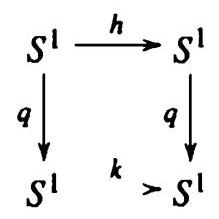
\includegraphics[width=0.2\textwidth]{images/57.0.jpg}
\end{center}
\hspace*{3em} 

Second, we note that if \(\widetilde{f}\) is any path in \({S}^{1}\) from \({b}_{0}\) to \(- {b}_{0}\) , then the loop \(f = q \circ  \widetilde{f}\) represents a nontrivial element of \({\pi }_{1}( {{S}^{1},{b}_{0}})\) . For \(\widetilde{f}\) is a lifting of \(f\) to \({S}^{1}\) that begins at \({b}_{0}\) and does not end at \({b}_{0}\) .

Finally, we show \({k}_{ * }\) is nontrivial. Let \(\widetilde{f}\) be a path in \({S}^{1}\) from \({b}_{0}\) to \(- {b}_{0}\) , and let \(f\) be the loop \(q \circ  \bar{f}\) . Then \({k}_{ * }[  f]\) is not trivial, for \({k}_{ * }[  f]   = [  {k \circ  ( {q \circ  \widetilde{f}}) }]   = [  {q \circ  ( {h \circ  \bar{f}}) }]\) ; the latter is nontrivial because \(h \circ  \bar{f}\) is a path in \({S}^{1}\) from \({b}_{0}\) to \(- {b}_{0}\) .

Step 3. Finally, we show that the homomorphism \({h}_{ * }\) is nontrivial, so that \(h\) cannot be nulhomotopic.

The homomorphism \({k}_{ * }\) is injective, being a nontrivial homomorphism of an infinite cyclic group with itself. The homomorphism \({q}_{ * }\) is also injective; indeed, \({q}_{ * }\) corresponds to multiplication by two in the group of integers. It follows that \({k}_{ * } \circ  {q}_{ * }\) is injective. Since \({q}_{ * } \circ  {h}_{ * } = {k}_{ * } \circ  {q}_{ * }\) , the homomorphism \({h}_{ * }\) must be injective as well.

\begin{center}
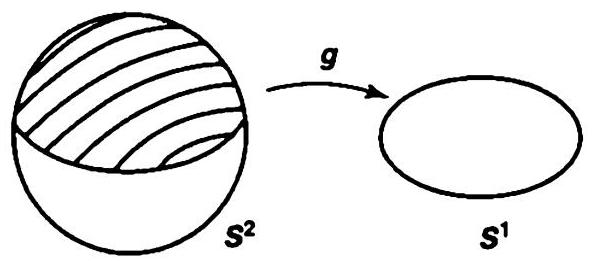
\includegraphics[width=0.5\textwidth]{images/57.1.jpg}
\end{center}
\hspace*{3em} 

Figure 57.1
\end{proof}
\begin{theorem}
	There is no continuous antipode-preserving map \(g : {S}^{2} \rightarrow  {S}^{1}\) .
\end{theorem}

\begin{proof}
	Suppose \(g : {S}^{2} \rightarrow  {S}^{1}\) is continuous and antipode preserving. Let us take \({S}^{1}\) to be the equator of \({S}^{2}\) . Then the restriction of \(g\) to \({S}^{1}\) is a continuous antipode-preserving map \(h\) of \({S}^{1}\) to itself. By the preceding theorem, \(h\) is not nulhomotopic. But the upper hemisphere \(E\) of \({S}^{2}\) is homeomorphic to the ball \({B}^{2}\) , and \(g\) is a continuous extension of \(h\) to \(E\) ! See Figure 57.1.
\end{proof}
\begin{theorem}[Borsuk-Ulam theorem for \({S}^{2}\)]
	Given a continuous map \(f : {S}^{2} \rightarrow\)  \({\mathbb{R}}^{2}\) , there is a point \(x\) of \({S}^{2}\) such that \(f( x)  = f( {-x})\) .
\end{theorem}

\begin{proof}
	Suppose that \(f( x)  \neq  f( {-x})\) for all \(x \in  {S}^{2}\) . Then the map
\[
g( x)  = [  {f( x)  - f( {-x}) }]  /\parallel f( x)  - f( {-x}) \parallel
\]

is a continuous map \(g : {S}^{2} \rightarrow  {S}^{1}\) such that \(g( {-x})  =  - g( x)\) for all \(x\) .
\end{proof}
\begin{theorem}[The \index{Bisection theorem}]
	Given two bounded polygonal regions in \({\mathbb{R}}^{2}\) , there exists a line in \({\mathbb{R}}^{2}\) that bisects each of them.
\end{theorem}

\begin{proof}
	We take two bounded polygonal regions \({A}_{1}\) and \({A}_{2}\) in the plane \({\mathbb{R}}^{2} \times  1\) in \({\mathbb{R}}^{3}\) , and show there is a line \(L\) in this plane that bisects each of them.
Given a point \(u\) of \({S}^{2}\) , let us consider the plane \(P\) in \({\mathbb{R}}^{3}\) passing through the origin that has \(u\) as its unit normal vector. This plane divides \({\mathbb{R}}^{3}\) into two half-spaces; let \({f}_{i}( u)\) equal the area of that portion of \({A}_{i}\) that lies on the same side of \(P\) as does the vector \(u\) .

If \(u\) is the unit vector \(\mathbf{k}\) , then \({f}_{i}( u)  = \operatorname{area}{A}_{i}\) ; and if \(u =  - \mathbf{k}\) , then \({f}_{i}( u)  = 0\) . Otherwise, the plane \(P\) intersects the plane \({\mathbb{R}}^{2} \times  1\) in a line \(L\) that splits \({\mathbb{R}}^{2} \times  1\) into two half-planes, and \({f}_{i}( u)\) is the area of that part of \({A}_{i}\) that lies on one side of this line. See Figure 57.2.

\begin{center}
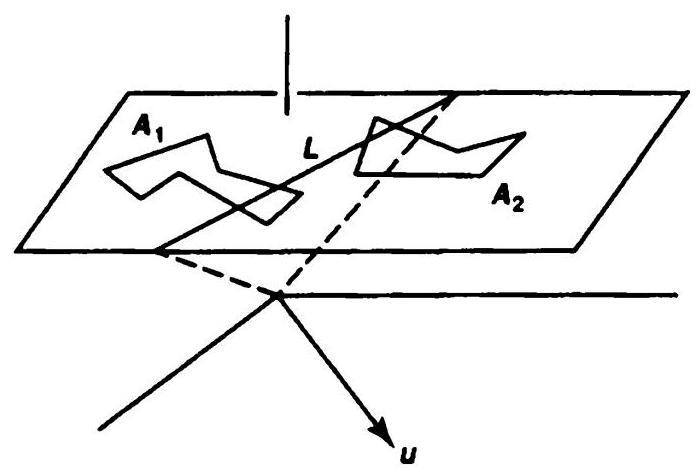
\includegraphics[width=0.6\textwidth]{images/57.2.jpg}
\end{center}
\hspace*{3em} 

Figure 57.2

Replacing \(u\) by \(- u\) gives us the same plane \(P\) , but the other half-space, so that \({f}_{i}( {-u})\) is the area of that part of \({A}_{i}\) that lies on the other side of \(P\) from \(u\) . It follows that

\[
{f}_{i}( u)  + {f}_{i}( {-u})  = \operatorname{area}{A}_{i}.
\]

Now consider the map \(F : {S}^{2} \rightarrow  {\mathbb{R}}^{2}\) given by \(F( u)  = ( {{f}_{1}( u) ,{f}_{2}( u) })\) . The Borsuk-Ulam theorem gives us a point \(u\) of \({S}^{2}\) for which \(F( u)  = F( {-u})\) . Then \({f}_{i}( u)  = {f}_{i}( {-u})\) for \(i = 1,2\) , that \({f}_{i}( u)  = \frac{1}{2}\) area \({A}_{i}\) , as desired.

We have proved the \index{bisection theorem@Bisection theorem}bisection theorem for bounded polygonal regions in the plane. However, all that was needed in the proof was the existence of an additive area function for \({A}_{1}\) and \({A}_{2}\) . Thus, the theorem holds for any two sets \({A}_{1}\) and \({A}_{2}\) that are ``Jordan-measurable'' in the sense used in analysis.

These theorems generalize to higher dimensions, but the proofs are considerably more sophisticated. The generalized version of the bisection theorem states that given \(n\) Jordan-measurable sets in \({\mathbb{R}}^{n}\) , there exists a plane of dimension \(n - 1\) that bisects them all. In the case \(n = 3\) , this result goes by the pleasant name of the ``\index{Ham sandwich theorem}.'' If one considers a ham sandwich to consist of two pieces of bread and a slab of ham, then the bisection theorem says that one can divide each of them precisely in half with a single whack of a cleaver \({}^{1}\)
\end{proof}
\section*{Exercises}
\begin{enumerate}[itemsep=0.4em, parsep=0pt, topsep=0pt, partopsep=0pt, leftmargin=*, label=\arabic*., ref=\arabic*]
\item Prove the following ``theorem of meteorology'': At any given moment in time, there exists a pair of antipodal points on the surface of the earth at which both the temperature and the barometric pressure are equal.
\item Show that if \(g : {S}^{2} \rightarrow  {S}^{2}\) is continuous and \(g( x)  \neq  g( {-x})\) for all \(x\) , then \(g\) is surjective. [Hint: If \(p \in  {S}^{2}\) , then \({S}^{2} - \{ p\}\) is homeomorphic to \({\mathbb{R}}^{2}\) .]
\item Let \(h : {S}^{1} \rightarrow  {S}^{1}\) be continuous and antipode-preserving with \(h( {b}_{0})  = {b}_{0}\) . Show that \({h}_{ * }\) carries a generator of \({\pi }_{1}( {{S}^{1},{b}_{0}})\) to an odd power of itself. [Hint: If \(k\) is the map constructed in the proof of Theorem 57.1, show that \({k}_{ * }\) does the same.]
\item Suppose you are given the fact that for each \(n\) , no continuous antipode-preserving map \(h : {S}^{n} \rightarrow  {S}^{n}\) is nulhomotopic. (This result can be proved using more advanced techniques of algebraic topology.) Prove the following:
  \begin{enumerate}[itemsep=0.2em, parsep=0pt, topsep=0pt, partopsep=0pt, leftmargin=*, label=(\alph*), align=left]
  \item There is no retraction \(r : {B}^{n + 1} \rightarrow  {S}^{n}\) .
  \item There is no continuous antipode-preserving map \(g : {S}^{n + 1} \rightarrow  {S}^{n}\) .
  \item (Borsuk-Ulam theorem) Given a continuous map \(f : {S}^{n + 1} \rightarrow  {\mathbb{R}}^{n + 1}\) , there is a point \(x\) of \({S}^{n + 1}\) such that \(f( x)  = f( {-x})\) .
  \item If \({A}_{1},\ldots ,{A}_{n + 1}\) are bounded measurable sets in \({\mathbb{R}}^{n + 1}\) , there exists an \(n\) - plane in \({\mathbb{R}}^{n + 1}\) that bisects each of them.
  \end{enumerate}
\end{enumerate}
\section*{§ 58 Deformation Retracts and Homotopy Type}

\index{deformation retract@Deformation Retract} As we have seen, one way of obtaining information about the fundamental group of a space \(X\) is to study the covering spaces of \(X\) . Another is one we discuss in this section, which involves the notion of \index{Homotopy type}. It provides a method for reducing the problem of computing the fundamental group of a space to that of computing the fundamental group of some other space-preferably, one that is more familiar.

We begin with a lemma.

\begin{lemma}
	Let \(h,k.( {X,{x}_{0}})  \rightarrow  ( {Y,{y}_{0}})\) be continuous maps. If \(h\) and \(k\) are homotopic, and if the image of the base point \({x}_{0}\) of \(X\) remains fixed at \({y}_{0}\) during the homotopy, then the homomorphisms \({h}_{ * }\) and \({k}_{ * }\) are equal.
\end{lemma}

\begin{proof}
	The proof is immediate. By assumption, there is a homotopy \(H : X \times  I \rightarrow  Y\) between \(h\) and \(k\) such that \(H( {{x}_{0},t})  = {y}_{0}\) for all \(t\) . It follows that if \(f\) is a loop in \(X\) based at \({x}_{0}\) , then the composite
\[
I \times  I\xrightarrow[]{f \times  \mathrm{{id}}}X \times  I\xrightarrow[]{H}Y
\]

is a homotopy between \(h \circ  f\) and \(k \circ  f\) ; it is a path homotopy because \(f\) is a loop at \({x}_{0}\) and \(H\) maps \({x}_{0} \times  l\) to \({y}_{0}\) .

Using this lemma, we generalize a result about the space \({\mathbb{R}}^{2} - \mathbf{0}\) proved earlier, proving that the homomorphism induced by inclusion \(j : {S}^{1} \rightarrow  {\mathbb{R}}^{2} - \mathbf{0}\) is not only injective but surjective as well. More generally, we prove the following:
\end{proof}
\begin{theorem}
	The inclusion map \(j : {S}^{n} \rightarrow  {\mathbb{R}}^{n + 1} - \mathbf{0}\) induces an isomorphism of fundamental groups.
\end{theorem}

\begin{proof}
	Let \(X = {\mathbb{R}}^{n + 1} - \mathbf{0}\) ; let \({b}_{0} = ( {1,0,\ldots ,0})\) . Let \(r : X \rightarrow  {S}^{n}\) be the map \(r( x)  = x/\parallel x\parallel\) . Then \(r \circ  j\) is the identity map of \({S}^{n}\) , so that \({r}_{ * } \circ  {j}_{ * }\) is the identity homomorphism of \({\pi }_{1}( {{S}^{n},{b}_{0}})\) .
Now consider the composite \(j \circ  r\) , which maps \(X\) to itself;

\[
X\overset{r}{ \rightarrow  }{S}^{n}\overset{j}{ \rightarrow  }X
\]

This map is not the identity map of \(X\) , but it is homotopic to the identity map. Indeed, the straight-line homotopy \(H : X \times  I \rightarrow  X\) , given by

\[
H( {x,t})  = ( {1 - t}) x + {tx}/\parallel x\parallel ,
\]

is a homotopy between the identity map of \(X\) and the map \(j \circ  r\) . For \(H( {x,t})\) is never equal to0, because \(( {1 - t})  + t/\parallel x\parallel\) is a number between 1 and \(1/\parallel x\parallel\) . Note that the point \({b}_{0}\) remains fixed during the homotopy, since \(\begin{Vmatrix}{b}_{0}\end{Vmatrix} = 1\) . It follows from the preceding lemma that the homomorphism \({( j \circ  r) }_{ * } = {j}_{ * } \circ  {r}_{ * }\) is the identity homomorphism of \({\pi }_{1}( {X,{b}_{0}})\) .

What made the preceding proof work? Roughly speaking, it worked because we had a natural way of deforming the identity map of \({\mathbb{R}}^{n + 1} - 0\) to a map that collapsed all of \({\mathbb{R}}^{n + 1} - \mathbf{0}\) onto \({S}^{n}\) . The deformation \(H\) gradually collapsed each radial line emanating from the origin to the point where it intersected \({S}^{n}\) ; each point of \({S}^{n}\) remained fixed during this deformation.

Figure 58.1 illustrates, in the case \(n = 1\) , how the deformation \(H\) gives rise to a path homotopy \(H( {f( s) ,t})\) between the loop \(f\) in \({\mathbb{R}}^{2} - \mathbf{0}\) and the loop \(g = f/\parallel f\parallel\) in \({S}^{1}\) .

% \begin{center}
% 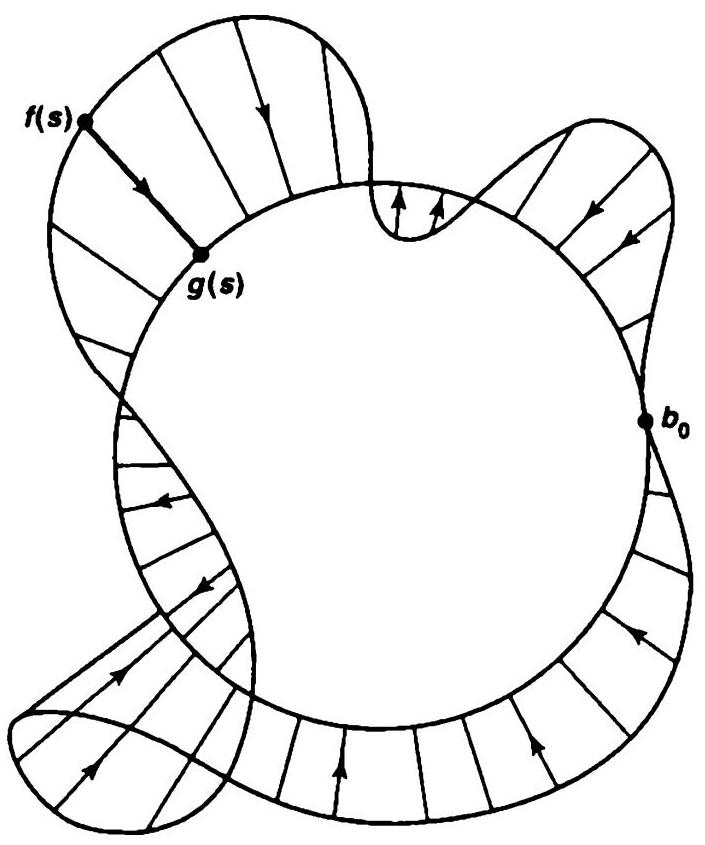
\includegraphics[width=0.6\textwidth]{images/58.1.jpg}
% \end{center}
\hspace*{3em} 

Figure 58.1

These comments lead us to formulate a more general situation in which the same procedure applies.
\end{proof}
\begin{definition}
	Let \(A\) be a subspace of \(X\) . We say that \(A\) is a deformation retract of \(X\) if the identity map of \(X\) is homotopic to a map that carries all of \(X\) into \(A\) , such that each point of \(A\) remains fixed during the homotopy. This means that there is a continuous map \(H : X \times  I \rightarrow  X\) such that \(H( {x,0})  = x\) and \(H( {x,1})  \in  A\) for all \(x \in  X\) , and \(H( {a,t})  = a\) for all \(a \in  A\) . The homotopy \(H\) is called a \index{Deformation retraction} of \(X\) onto \(A\) . The map \(r : X \rightarrow  A\) defined by the equation \(r( x)  = H( {x,1})\) is a retraction of \(X\) onto \(A\) , and \(H\) is a homotopy between the identity map of \(X\) and the map \(j \circ  r\) , where \(j : A \rightarrow  X\) is inclusion.
\end{definition}

The proof of the preceding theorem generalizes immediately to prove the following:

\begin{theorem}
	Let \(A\) be a deformation retract of \(X\) ; let \({x}_{0} \in  A\) . Then the inclusion map

\[
j : ( {A,{x}_{0}})  \rightarrow  ( {X,{x}_{0}})
\]

induces an isomorphism of fundamental groups.
\end{theorem}

\end{example}
\end{centeredblock}

\begin{centeredblock}
\begin{example}
	Let \(B\) denote the \(z\) -axis in \({\mathbb{R}}^{3}\) Consider the space \({\mathbb{R}}^{3} - B\) It has the punctured \({xy}\) -plane \(( {{\mathbb{R}}^{2} - 0})  \times  0\) as a \index{deformation retract@Deformation retract}deformation retract The map \(H\) defined by the equation

\[
H( {x,y,z,t})  = ( {x,y,( {1 - t}) z})
\]

is a \index{deformation retraction@Deformation retraction}deformation retraction; it gradually collapses each line parallel to the \(z\) -axis into the point where the line intersects the \({xy}\) -plane. We conclude that the space \({\mathbb{R}}^{3} - B\) has an infinite cyclic fundamental group.

\end{example}
\end{centeredblock}

\begin{centeredblock}
\begin{example}
	Consider \({\mathbb{R}}^{2} - p - q\) , the \index{Doubly punctured plane}. We assert it has the ``figure eight'' space as a deformation retract. Rather than writing equations, we merely sketch the deformation retraction; it is the three-stage deformation indicated in Figure 58.2.

\begin{center}
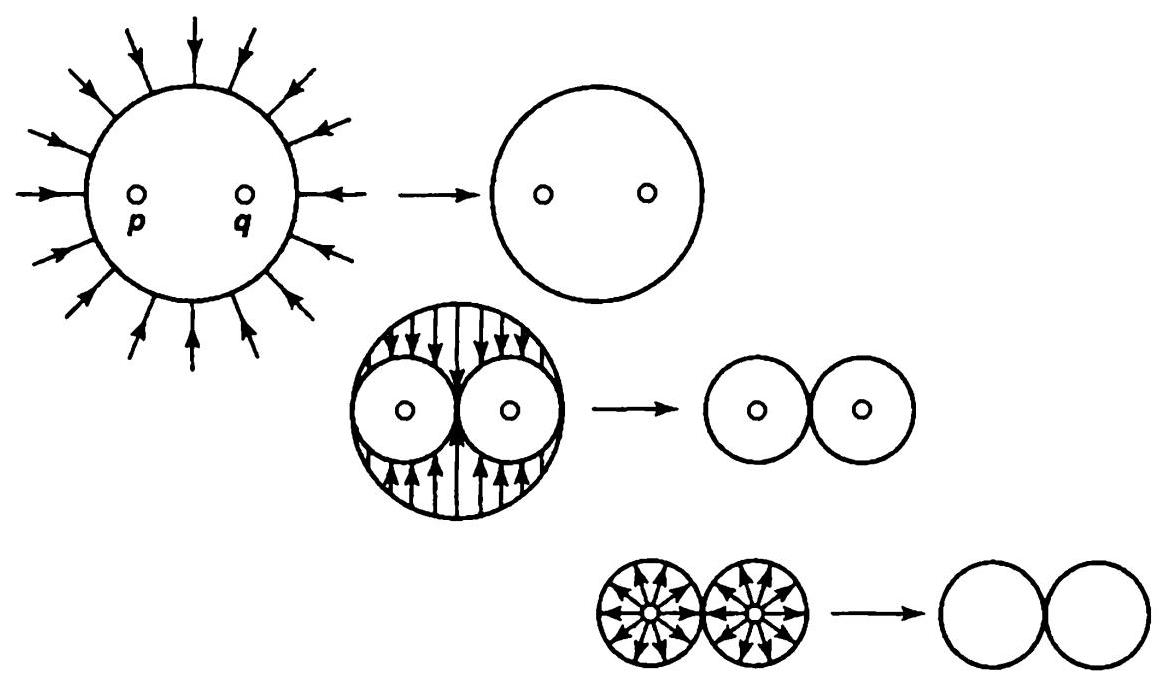
\includegraphics[width=1.0\textwidth]{images/58.2.jpg}
\end{center}
\hspace*{3em} 

Figure 58.2

\end{example}
\end{centeredblock}

\begin{centeredblock}
\begin{example}
	Another deformation retract of \({\mathbb{R}}^{2} - p - q\) is the ``\index{Theta space}''

\[
\theta  = {S}^{1} \cup  ( {0 \times  [  {-1,1}]  })
\]

we leave it to you to sketch the maps involved. As a result, the figure eight and the \index{theta space@Theta space}theta space have isomorphic fundamental groups, even though neither is a deformation retract of the other.
\end{example}
\end{centeredblock}

Of course, we do not know anything about the fundamental group of the figure eight as yet. But we shall.

The example of the figure eight and the theta space suggests the possibility that there might be a more general way of showing two spaces have isomorphic fundamental groups than by showing that one is homeomorphic to a deformation retract of the other. We formulate such a notion now.

\begin{definition}
	Let \(f : X \rightarrow  Y\) and \(g : Y \rightarrow  X\) be continuous maps. Suppose that the map \(g \circ  f : X \rightarrow  X\) is homotopic to the identity map of \(X\) , and the map \(f \circ  g : Y \rightarrow  Y\) is homotopic to the identity map of \(Y\) . Then the maps \(f\) and \(g\) are called homotopy equivalences, and each is said to be a \index{Homotopy inverse} of the other.
\end{definition}

It is straightforward to show that if \(f : X \rightarrow  Y\) is a homotopy equivalence of \(X\) with \(Y\) and \(h : Y \rightarrow  Z\) is a homotopy equivalence of \(Y\) with \(Z\) , then \(h \circ  f : X \rightarrow  Z\) is a homotopy equivalence of \(X\) with \(Z\) . It follows that the relation of homotopy equivalence is an equivalence relation. Two spaces that are homotopy equivalent are said to have the same homotopy type.

Note that if \(A\) is a deformation retract of \(X\) , then \(A\) has the same homotopy type as \(X\) . For let \(j : A \rightarrow  X\) be the inclusion mapping and let \(r : X \rightarrow  A\) be the retraction mapping. Then the composite \(r \circ  j\) equals the identity map of \(A\) , and the composite \(j \circ  r\) is by hypothesis homotopic to the identity map of \(X\) (and in fact each point of \(A\) remains fixed during the homotopy).

We now show that two spaces having the same homotopy type have isomorphic fundamental groups. For this purpose, we need to study what happens when we have a homotopy between two continuous maps of \(X\) into \(Y\) such that the base point of \(X\) does not remain fixed during the homotopy.

\begin{lemma}
	Let \(h,k : X \rightarrow  Y\) be continuous maps; let \(h( {x}_{0})  = {y}_{0}\) and \(k( {x}_{0})  = {y}_{1}\) . If \(h\) and \(k\) are homotopic, there is a path \(\alpha\) in \(Y\) from \({y}_{0}\) to \({y}_{1}\) such that \({k}_{ * } = \widehat{\alpha } \circ  {h}_{ * }\) . Indeed, if \(H : X \times  I \rightarrow  Y\) is the homotopy between \(h\) and \(k\) , then \(\alpha\) is the path \(\alpha ( t)  = H( {{x}_{0},t})\) .
\end{lemma}

\begin{center}
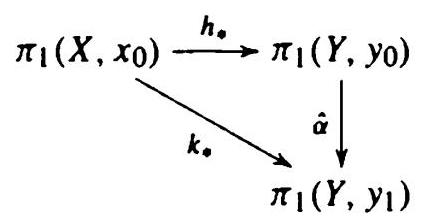
\includegraphics[width=0.3\textwidth]{images/58.25.jpg}
\end{center}
\hspace*{3em} 

\begin{proof}
	Let \(f : I \rightarrow  X\) be a loop in \(X\) based at \({x}_{0}\) . We must show that
\[
{k}_{ * }( [  f]  )  = \widehat{\alpha }( {h}_{ * }( [  f]  ) )
\]

This equation states that \([  {k \circ  f}]   = [  \bar{\alpha }]   * [  {h \circ  f}]   * [  \alpha ]\) , or equivalently, that

\[
[  \alpha ]   * [  {k \circ  f}]   = [  {h \circ  f}]   * [  \alpha ]  .
\]

This is the equation we shall verify.

To begin, consider the loops \({f}_{0}\) and \({f}_{1}\) in the space \(X \times  I\) given by the equations

\[
{f}_{0}( s)  = ( {f( s) ,0}) \;\text{ and }\;{f}_{1}( s)  = ( {f( s) ,1}) .
\]

Consider also the path \(c\) in \(X \times  I\) given by the equation

\[
c( t)  = ( {{x}_{0},t}) \text{ . }
\]

\begin{center}
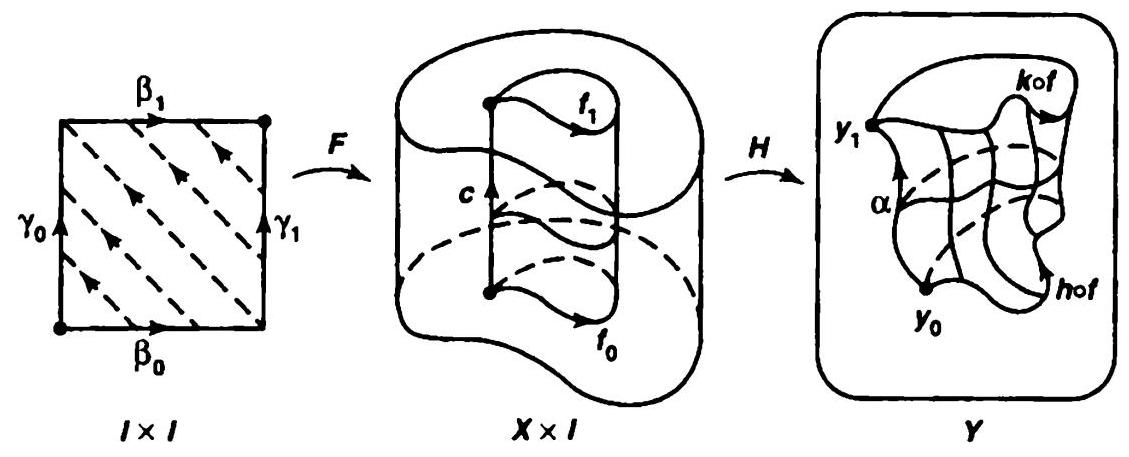
\includegraphics[width=1.0\textwidth]{images/58.3.jpg}
\end{center}
\hspace*{3em} 

Figure 58.3

Then \(H \circ  {f}_{0} = h \circ  f\) and \(H \circ  {f}_{1} = k \circ  f\) , while \(H \circ  c\) equals the path \(\alpha\) . See Figure 58.3.

Let \(F : I \times  I \rightarrow  X \times  I\) be the map \(F( {s,t})  = ( {f( s) ,t})\) . Consider the following paths in \(I \times  I\) , which run along the four edges of \(I \times  I\) :

\[
{\beta }_{0}( s)  = ( {s,0}) \;\text{ and }\;{\beta }_{1}( s)  = ( {s,1}) ,
\]

\[
{\gamma }_{0}( t)  = ( {0,t}) \;\text{ and }\;{\gamma }_{1}( t)  = ( {1,t}) .
\]

Then \(F \circ  {\beta }_{0} = {f}_{0}\) and \(F \circ  {\beta }_{1} = {f}_{1}\) , while \(F \circ  {\gamma }_{0} = F \circ  {\gamma }_{1} = c\) .

The broken-line paths \({\beta }_{0} * {\gamma }_{1}\) and \({\gamma }_{0} * {\beta }_{1}\) are paths in \(I \times  I\) from(0,0)to(1,1); since \(I \times  I\) is convex, there is a path homotopy \(G\) between them. Then \(F \circ  G\) is a path homotopy in \(X \times  I\) between \({f}_{0} * c\) and \(c * {f}_{1}\) . And \(H \circ  ( {F \circ  G})\) is a path homotopy in \(Y\) between

\[
( {H \circ  {f}_{0}})  * ( {H \circ  c})  = ( {h \circ  f})  * \alpha \;\text{ and }
\]

\[
( {H \circ  c})  * ( {H \circ  {f}_{1}})  = \alpha  * ( {k \circ  f}) ,
\]

as desired.
\end{proof}
\begin{corollary}
	Let \(h,k : X \rightarrow  Y\) be homotopic continuous maps; let \(h( {x}_{0})  = {y}_{0}\) and \(k( {x}_{0})  = {y}_{1}\) . If \({h}_{ * }\) is injective, or surjective, or trivial, so is \({k}_{ * }\) .
\end{corollary}

\begin{corollary}
	Let \(h : X \rightarrow  Y\) . If \(h\) is nulhomotopic, then \({h}_{ * }\) is the trivial homomorphism.
\end{corollary}

\begin{proof}
	The constant map induces the trivial homomorphism.
\end{proof}
\begin{theorem}
	Let \(f : X \rightarrow  Y\) be continuous; let \(f( {x}_{0})  = {y}_{0}\) . If \(f\) is a \index{homotopy equivalence@Homotopy equivalence}homotopy equivalence, then

\[
{f}_{ * } : {\pi }_{1}( {X,{x}_{0}})  \rightarrow  {\pi }_{1}( {Y,{y}_{0}})
\]

is an isomorphism.
\end{theorem}

\begin{proof}
	Let \(g : Y \rightarrow  X\) be a homotopy inverse for \(f\) . Consider the maps
\[
( {X,{x}_{0}}) \overset{f}{ \rightarrow  }( {Y,{y}_{0}}) \overset{g}{ \rightarrow  }( {X,{x}_{1}}) \overset{f}{ \rightarrow  }( {Y,{y}_{1}}) ,
\]

where \({x}_{1} = g( {y}_{0})\) and \({y}_{1} = f( {x}_{1})\) . We have the corresponding induced homomorphisms:

\begin{center}
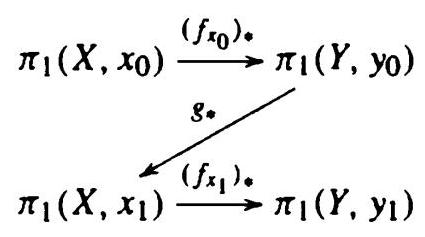
\includegraphics[width=0.3\textwidth]{images/58.35.jpg}
\end{center}
\hspace*{3em} 

[Here we have to distinguish between the homomorphisms induced by \(f\) relative to two different base points.] Now

\[
g \circ  f : ( {X,{x}_{0}})  \rightarrow  ( {X,{x}_{1}})
\]

is by hypothesis homotopic to the identity map, so there is a path \(\alpha\) in \(X\) such that

\[
{( g \circ  f) }_{ * } = \widehat{\alpha } \circ  {( i\chi ) }_{ * } = \widehat{\alpha }.
\]

It follows that \({( g \circ  f) }_{ * } = {g}_{ * } \circ  {( {f}_{{x}_{0}}) }_{ * }\) is an isomorphism.

Similarly, because \(f \circ  g\) is homotopic to the identity map \({iy}\) , the homomorphism \({( f \circ  g) }_{ * } = {( {f}_{{x}_{1}}) }_{ * } \circ  {g}_{ * }\) is an isomorphism.

The first fact implies that \({g}_{ * }\) is surjective, and the second implies that \({g}_{ * }\) is injective. Therefore, \({g}_{ * }\) is an isomorphism. Applying the first equation once again, we conclude that

\[
{( {f}_{{x}_{0}}) }_{ * } = {( {g}_{ * }) }^{-1} \circ  \widehat{\alpha },
\]

so that \({( {f}_{{x}_{0}}) }_{ * }\) is also an isomorphism.

Note that although \(g\) is a \index{homotopy inverse@Homotopy inverse}homotopy inverse for \(f\) , the homomorphism \({g}_{ * }\) is not an inverse for the homomorphism \({( {f}_{{x}_{0}}) }_{ * }\) .

The relation of homotopy equivalence is clearly more general than the notion \index{Fundamental group!of deformation retract}of deformation retraction. The theta space and the figure eight are both deformation retracts of the \index{doubly punctured plane@Doubly punctured plane}doubly punctured plane. Therefore, they are homotopy equivalent to the doubly punctured plane, and hence to each other. But neither is homeomorphic to a deformation retract of the other; in fact, neither of them can even be imbedded in the other.

It is a striking fact that the situation that occurs for these two spaces is the standard situation regarding homotopy equivalences. Martin Fuchs has proved a theorem to the effect that two spaces \(X\) and \(Y\) have the same \index{Contractible space!homotopy type}homotopy type if and only if they are homeomorphic to deformation retracts of a single space \(Z\) . The proof, although it uses only elementary tools, is difficult 		\cite{Fuchs1971}.
\end{proof}
\section*{Exercises}
\begin{enumerate}[itemsep=0.4em, parsep=0pt, topsep=0pt, partopsep=0pt, leftmargin=*, label=\arabic*., ref=\arabic*]
\item Show that if \(A\) is a deformation retract of \(X\) , and \(B\) is a deformation retract of \(A\) , then \(B\) is a deformation retract of \(X\) .
\item For each of the following spaces, the fundamental group is either trivial, infinite cyclic, or isomorphic to the fundamental group of the figure eight. Determine for each space which of the three alternatives holds.
  \begin{enumerate}[itemsep=0.2em, parsep=0pt, topsep=0pt, partopsep=0pt, leftmargin=*, label=(\alph*), align=left]
  \item The ``solid torus,'' \({B}^{2} \times  {S}^{1}\) .
  \item The torus \(T\) with a point removed.
  \item The cylinder \({S}^{1} \times  I\) .
  \item The infinite cylinder \({S}^{1} \times  \mathbb{R}\) .
  \item \({\mathbb{R}}^{3}\) with the nonnegative \(x,y\) , and \(z\) axes deleted. The following subsets of \({\mathbb{R}}^{2}\) :
  \item \(\{ x \mid  \parallel x\parallel  > 1\}\)
  \item \(\{ x \mid  \parallel x\parallel  \geq  1\}\)
  \item \(\{ x \mid  \parallel x\parallel  < 1\}\)
  \item \({S}^{1} \cup  ( {{\mathbb{R}}_{ + } \times  0})\)
  \item \({S}^{1} \cup  ( {{\mathbb{R}}_{ + } \times  \mathbb{R}})\)
  \item \({S}^{1} \cup  ( {\mathbb{R} \times  0})\)
  \item \({\mathbb{R}}^{2} - ( {{\mathbb{R}}_{ + } \times  0})\)
  \end{enumerate}
\item Show that given a collection \(\mathcal{C}\) of spaces, the relation of homotopy equivalence is an equivalence relation on \(\mathcal{C}\) .
\item Let \(X\) be the figure eight and let \(Y\) be the theta space. Describe maps \(f : X \rightarrow  Y\) and \(g : Y \rightarrow  X\) that are homotopy inverse to each other.
\item Recall that a space \(X\) is said to be contractible if the identity map of \(X\) to itself is nulhomotopic. Show that \(X\) is contractible if and only if \(X\) has the homotopy type of a one-point space.
\item Show that a retract of a contractible space is contractible.
\item Let \(A\) be a subspace of \(X\) ; let \(j : A \rightarrow  X\) be the inclusion map, and let \(f : X \rightarrow\)  \(A\) be a continuous map. Suppose there is a homotopy \(H : X \times  I \rightarrow  X\) between the map \(j \circ  f\) and the identity map of \(X\) .
  \begin{enumerate}[itemsep=0.2em, parsep=0pt, topsep=0pt, partopsep=0pt, leftmargin=*, label=(\alph*), align=left]
  \item Show that if \(f\) is a retraction, then \({j}_{ * }\) is an isomorphism.
  \item Show that if \(H\) maps \(A \times  I\) into \(A\) , then \({j}_{ * }\) is an isomorphism.
  \item Give an example in which \({j}_{ * }\) is not an isomorphism. *8. Find a space \(X\) and a point \({x}_{0}\) of \(X\) such that inclusion \(\{  {x}_{0}\}   \rightarrow  X\) is a homotopy equivalence, but \(\{  {x}_{0}\}\) is not a deformation retract of \(X\) . [Hint: Let \(X\) be the subspace of \({\mathbb{R}}^{2}\) that is the union of the line segments \(( {1/n})  \times  I\) , for \(n \in  {\mathbb{Z}}_{ + }\) , the line segment \(0 \times  I\) , and the line segment \(I \times  0\) ; let \({x}_{0}\) be the point(0,1). If \(\{  {x}_{0}\}\) is a deformation retract of \(X\) , show that for any neighborhood \(U\) of \({x}_{0}\) , the path component of \(U\) containing \({x}_{0}\) contains a neighborhood of \({x}_{0}\) .]
  \end{enumerate}
\item We define the degree of a continuous map \(h : {S}^{1} \rightarrow  {S}^{1}\) as follows: Let \({b}_{0}\) be the point(1,0)of \({S}^{1}\) ; choose a generator \(\gamma\) for the infinite cyclic group \({\pi }_{1}( {{S}^{1},{b}_{0}})\) . If \({x}_{0}\) is any point of \({S}^{1}\) , choose a path \(\alpha\) in \({S}^{1}\) from \({b}_{0}\) to \({x}_{0}\) , and define \(\gamma ( {x}_{0})  = \widehat{\alpha }( \gamma )\) . Then \(\gamma ( {x}_{0})\) generates \({\pi }_{1}( {{S}^{1},{x}_{0}})\) . The element \(\gamma ( {x}_{0})\) is independent of the choice of the path \(\alpha\) , since the fundamental group of \({S}^{1}\) is abelian. Now given \(h : {S}^{1} \rightarrow  {S}^{1}\) , choose \({x}_{0} \in  {S}^{1}\) and let \(h( {x}_{0})  = {x}_{1}\) . Consider the homomorphism \[ {h}_{ * } : {\pi }_{1}( {{S}^{1},{x}_{0}})  \rightarrow  {\pi }_{1}( {{S}^{1},{x}_{1}}) . \] Since both groups are infinite cyclic, we have (*) \[ {h}_{ * }( {\gamma ( {x}_{0}) })  = d \cdot  \gamma ( {x}_{1}) \] for some integer \(d\) , if the group is written additively. The integer \(d\) is called the degree of \(h\) and is denoted by \(\deg h\) . The degree of \(h\) is independent of the choice of the generator \(\gamma\) ; choosing the other generator would merely change the sign of both sides of \(( *)\) .
  \begin{enumerate}[itemsep=0.2em, parsep=0pt, topsep=0pt, partopsep=0pt, leftmargin=*, label=(\alph*), align=left]
  \item Show that \(d\) is independent of the choice of \({x}_{0}\) .
  \item Show that if \(h,k : {S}^{1} \rightarrow  {S}^{1}\) are homotopic, they have the same degree.
  \item Show that \(\deg ( {h \circ  k})  = ( {\deg h})  \cdot  ( {\deg k})\) .
  \item Compute the degrees of the constant map, the identity map, the reflection map \(\rho ( {{x}_{1},{x}_{2}})  = ( {{x}_{1}, - {x}_{2}})\) , and the map \(h( z)  = {z}^{n}\) , where \(z\) is a complex number. *(e) Show that if \(h,k : {S}^{1} \rightarrow  {S}^{1}\) have the same degree, they are homotopic.
  \end{enumerate}
\item Suppose that to every map \(h : {S}^{n} \rightarrow  {S}^{n}\) we have assigned an integer, denoted by deg \(h\) and called the degree of \(h\) , such that:
  \begin{enumerate}[itemsep=0.2em, parsep=0pt, topsep=0pt, partopsep=0pt, leftmargin=*, label=(\alph*), align=left]
  \item \index{homotopic maps@Homotopic maps} have the same degree. (ii) \(\deg ( {h \circ  k})  = ( {\deg h})  \cdot  ( {\deg k})\) . (iii) The identity map has degree 1, any constant map has degree 0, and the reflection map \(\rho ( {{x}_{1},\ldots ,{x}_{n + 1}})  = ( {{x}_{1},\ldots ,{x}_{n}, - {x}_{n + 1}})\) has degree-1. [One can construct such a function, using the tools of algebraic topology. Intuitively, \(\deg h\) measures how many times \(h\) wraps \({S}^{n}\) about itself; the sign tells you whether \(h\) preserves orientation or not.] Prove the following:
  \item There is no retraction \(r : {B}^{n + 1} \rightarrow  {S}^{n}\) .
  \item If \(h : {S}^{n} \rightarrow  {S}^{n}\) has degree different from \({( -1) }^{n + 1}\) , then \(h\) has a fixed point. [Hint: Show that if \(h\) has no fixed point, then \(h\) is homotopic to the \index{Antipodal map} \(a( x)  =  - x\) .]
  \item If \(h : {S}^{n} \rightarrow  {S}^{n}\) has degree different from 1, then \(h\) maps some point \(x\) to its antipode \(- x\) .
  \item If \({S}^{n}\) has a nonvanishing tangent vector field \(v\) , then \(n\) is odd. [Hint: If \(v\) exists, show the identity map is homotopic to the \index{antipodal map@Antipodal map}antipodal map.]
  \end{enumerate}
\end{enumerate}
\section*{§ 59 The Fundamental Group of \({S}^{n}\)}

Now we turn to a problem mentioned at the beginning of the chapter, the problem of showing that the sphere, torus, and double torus are surfaces that are topologically distinct. We begin with the sphere; we show that \({S}^{n}\) is simply connected for \(n \geq  2\) . The crucial result we need is stated in the following theorem.

\begin{theorem}
	Suppose \(X = U \cup  V\) , where \(U\) and \(V\) are open sets of \(X\) . Suppose that \(U \cap  V\) is path connected, and that \({x}_{0} \in  U \cap  V\) . Let \(i\) and \(j\) be the inclusion mappings of \(U\) and \(V\) , respectively, into \(X\) . Then the images of the induced homomorphisms

\[
{i}_{ * } : {\pi }_{1}( {U,{x}_{0}})  \rightarrow  {\pi }_{1}( {X,{x}_{0}}) \;\text{ and }\;{j}_{ * } : {\pi }_{1}( {V,{x}_{0}})  \rightarrow  {\pi }_{1}( {X,{x}_{0}})
\]

generate \({\pi }_{1}( {X,{x}_{0}})\) .
\end{theorem}

\begin{proof}
	This theorem states that, given any loop \(f\) in \(X\) based at \({x}_{0}\) , it is path homotopic to a product of the form \(( {{g}_{1} * ( {{g}_{2} * ( {\cdots  * {g}_{n}}) }) })\) , where each \({g}_{i}\) is a loop in \(X\) based at \({x}_{0}\) that lies either in \(U\) or in \(V\) .
Step 1. We show there is a subdivision \({a}_{0} < {a}_{1} < \cdots  < {a}_{n}\) of the unit interval such that \(f( {a}_{i})  \in  U \cap  V\) and \(f( [  {{a}_{i - 1},{a}_{i}}]  )\) is contained either in \(U\) or in \(V\) , for each \(i\) .

To begin, choose a subdivision \({b}_{0},\ldots ,{b}_{m}\) of \([  {0,1}]\) such that for each \(i\) , the set \(f( [  {{b}_{i - 1},{b}_{i}}]  )\) is contained in either \(U\) or \(V\) . (Use the Lebesgue number lemma.) If \(f( {b}_{i})\) belongs to \(U \cap  V\) for each \(i\) , we are finished. If not, let \(i\) be an index such that \(f( {b}_{i})  \notin  U \cap  V\) . Each of the sets \(f( [  {{b}_{i - 1},{b}_{i}}]  )\) and \(f( [  {{b}_{i},{b}_{i + 1}}]  )\) lies either in \(U\) or in \(V\) . If \(f( {b}_{i})  \in  U\) , then both of these sets must lie in \(U\) ; and if \(f( {b}_{i})  \in  V\) , both of them must lie in \(V\) . In either case, we may delete \({b}_{i}\) , obtaining a new subdivision \({\mathrm{c}}_{0}\) , \(\ldots ,{c}_{m - 1}\) that still satisfies the condition that \(f( [  {{c}_{i - 1},{c}_{i}}]  )\) is contained either in \(U\) or in \(V\) , for each \(i\) .

A finite number of repetitions of this process leads to the desired subdivision.

Step 2. We prove the theorem. Given \(f\) , let \({a}_{0},\ldots ,{a}_{n}\) be the subdivision constructed in Step 1. Define \({f}_{i}\) to be the path in \(X\) that equals the positive linear map of \([  {0,1}]\) onto \([  {{a}_{i - 1},{a}_{i}}]\) followed by \(f\) . Then \({f}_{i}\) is a path that lies either in \(U\) or in \(V\) , and by Theorem 51.3,

\[
[  f]   = [  {f}_{1}]   * [  {f}_{2}]   * \cdots  * [  {f}_{n}]  .
\]

For each \(i\) , choose a path \({\alpha }_{i}\) in \(U \cap  V\) from \({x}_{0}\) to \(f( {a}_{i})\) . (Here we use the fact that \(U \cap  V\) is path connected.) Since \(f( {a}_{0})  = f( {a}_{n})  = {x}_{0}\) , we can choose \({\alpha }_{0}\) and \({\alpha }_{n}\) to be the constant path at \({x}_{0}\) . See Figure 59.1.

Now we set

\[
{g}_{i} = ( {{\alpha }_{i - 1} * {f}_{i}})  * \overline{{\alpha }_{i}}
\]

for each \(i\) . Then \({g}_{i}\) is a loop in \(X\) based at \({x}_{0}\) whose image lies either in \(U\) or in \(V\) Direct computation shows that

\[
[  {g}_{1}]   * [  {g}_{2}]   * \cdots  * [  {g}_{n}]   = [  {f}_{1}]   * [  {f}_{2}]   * \cdots  * [  {f}_{n}]  .
\]

\begin{center}
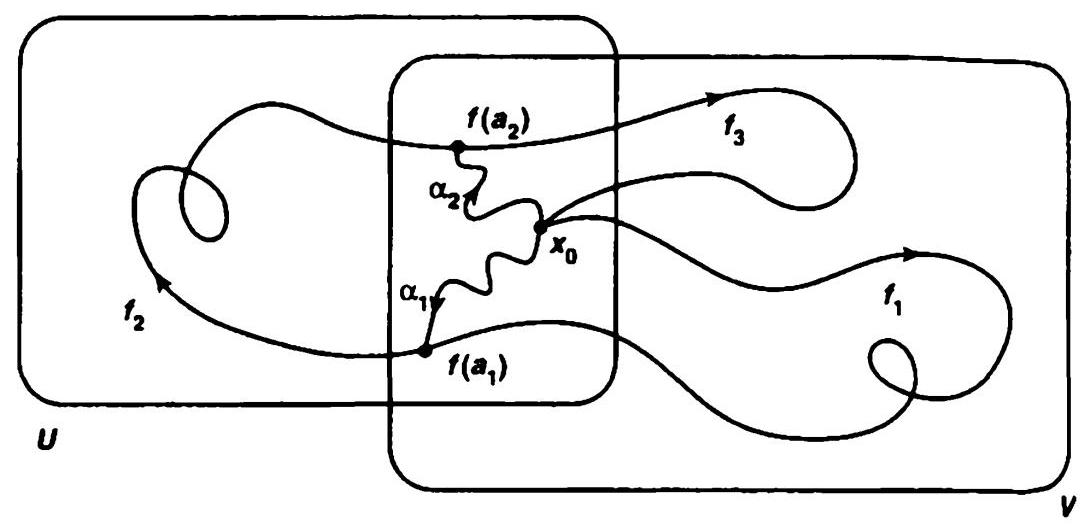
\includegraphics[width=1.0\textwidth]{images/59.1.jpg}
\end{center}
\hspace*{3em} 

Figure 59.1

The preceding theorem is a special case of a famous theorem of topology called the Seifert-van Kampen theorem, which expresses the fundamental group of the space \(X = U \cup  V\) quite generally, when \(U \cap  V\) is path connected, in terms of the fundamental groups of \(U\) and \(V\) . We shall study this theorem in \(C\) hapter 11 .
\end{proof}
\begin{corollary}
	Suppose \(X = U \cup  V\) , where \(U\) and \(V\) are open sets of \(X\) ; suppose \(U \cap  V\) is nonempty and path connected. If \(U\) and \(V\) are simply connected, then \(X\) is simply connected.
\end{corollary}

\begin{theorem}
	If \(n \geq  2\) , the \(n\) -sphere \({S}^{n}\) is \index{Simply connected!of \({S}^{n}\)}simply connected.
\end{theorem}

\begin{proof}
	Let \(p = ( {0,\ldots ,0,1})  \in  {\mathbb{R}}^{n + 1}\) and \(q = ( {0,\ldots ,0, - 1})\) be the ``north pole'' and the ``south pole'' of \({S}^{n}\) , respectively.
Step 1. We show that if \(n \geq  1\) , the punctured sphere \({S}^{n} - p\) is homeomorphic to \({\mathbb{R}}^{n}\) .

Define \(f : ( {{S}^{n} - p})  \rightarrow  {\mathbb{R}}^{n}\) by the equation

\[
f( x)  = f( {{x}_{1},\ldots ,{x}_{n + 1}})  = \frac{1}{1 - {x}_{n + 1}}( {{x}_{1},\ldots ,{x}_{n}}) .
\]

The map \(f\) is called \index{Stereographic projection}. (If one takes the straight line in \({\mathbb{R}}^{n + 1}\) passing through the north pole \(p\) and the point \(x\) of \({S}^{n} - p\) , then this line intersects the \(n\) -plane \({\mathbb{R}}^{n} \times  0 \subset  {\mathbb{R}}^{n + 1}\) in the point \(f( x)  \times  0\) .) One checks that \(f\) is a homeomorphism by showing that the map \(g : {\mathbb{R}}^{n} \rightarrow  ( {{S}^{n} - p})\) given by

\[
g( y)  = g( {{y}_{1},\ldots ,{y}_{n}})  = ( {t( y)  \cdot  {y}_{1},\ldots ,t( y)  \cdot  {y}_{n},1 - t( y) }) ,
\]

where \(t( y)  = 2/( {1 + \parallel y{\parallel }^{2}})\) , is a right and left inverse for \(f\) .

Note that the reflection map \(( {{x}_{1},\ldots ,{x}_{n + 1}})  \rightarrow  ( {{x}_{1},\ldots ,{x}_{n}, - {x}_{n + 1}})\) defines a homeomorphism of \({S}^{n} - p\) with \({S}^{n} - q\) , so the latter is also homeomorphic to \({\mathbb{R}}^{n}\) .

Step 2. We prove the theorem. Let \(U\) and \(V\) be the open sets \(U = {S}^{n} - p\) and \(V = {S}^{n} - q\) of \({S}^{n}.\)

Note first that for \(n \geq  1\) , the sphere \({S}^{n}\) is \index{Path connectedness!of \({S}^{n}\)}path connected. This follows from the fact that \(U\) and \(V\) are path connected (being homeomorphic to \({\mathbb{R}}^{n}\) ) and have the point \(( {1,0,\ldots ,0})\) of \({S}^{n}\) in common.

Now we show that for \(n \geq  2\) , the sphere \({S}^{n}\) is simply connected. The spaces \(U\) and \(V\) are simply connected, being homeomorphic to \({\mathbb{R}}^{n}\) . Their intersection equals \({S}^{n} - p - q\) , which is homeomorphic under \index{stereographic projection@Stereographic projection}stereographic projection to \({\mathbb{R}}^{n} - \mathbf{0}\) . The latter space is path connected, for every point of \({\mathbb{R}}^{n} - 0\) can be joined to a point of \({S}^{n - 1}\) by a straight-line path, and \({S}^{n - 1}\) is path connected if \(n \geq  2\) . Then the preceding corollary applies.
\end{proof}
\section*{Exercises}
\begin{enumerate}[itemsep=0.4em, parsep=0pt, topsep=0pt, partopsep=0pt, leftmargin=*, label=\arabic*., ref=\arabic*]
\item Let \(X\) be the union of two copies of \({S}^{2}\) having a single point in common. What is the fundamental group of \(X\) ? Prove that your answer is correct. [Be careful! The union of two simply connected spaces having a point in common is not necessarily simply connected. See 		\cite{Spanier1966}, p. 59.]
\item Criticize the following ``proof'' that \({S}^{2}\) is simply connected: Let \(f\) be a loop in \({S}^{2}\) based at \({x}_{0}\) . Choose a point \(p\) of \({S}^{2}\) not lying in the image of \(f\) . Since \({S}^{2} - p\) is homeomorphic with \({\mathbb{R}}^{2}\) , and \({\mathbb{R}}^{2}\) is simply connected, the loop \(f\) is path homotopic to the constant loop.
\item
  \begin{enumerate}[itemsep=0.2em, parsep=0pt, topsep=0pt, partopsep=0pt, leftmargin=*, label=(\alph*), align=left]
  \item Show that \({\mathbb{R}}^{1}\) and \({\mathbb{R}}^{n}\) are not homeomorphic if \(n > 1\) .

  \item Show that \({\mathbb{R}}^{2}\) and \({\mathbb{R}}^{n}\) are not homeomorphic if \(n > 2\) . It is, in fact, true that \({\mathbb{R}}^{m}\) and \({\mathbb{R}}^{n}\) are not homeomorphic if \(n \neq  m\) , but the proof requires more advanced tools of algebraic topology.
  \end{enumerate}
\item Assume the hypotheses of Theorem 59.1.
  \begin{enumerate}[itemsep=0.2em, parsep=0pt, topsep=0pt, partopsep=0pt, leftmargin=*, label=(\alph*), align=left]
  \item What can you say about the fundamental group of \(X\) if \({j}_{ * }\) is the trivial homomorphism? If both \({i}_{ * }\) and \({j}_{ * }\) are trivial?
  \item Give an example where \({i}_{ * }\) and \({j}_{ * }\) are trivial but neither \(U\) nor \(V\) have trivial fundamental groups
  \end{enumerate}
\end{enumerate}
\section*{§ 60 Fundamental Groups of Some Surfaces}

Recall that a surface is a Hausdorff space with a countable basis, each point of which has a neighborhood that is homeomorphic with an open subset of \({\mathbb{R}}^{2}\) . Surfaces are of interest in various parts of mathematics, including geometry, topology, and complex analysis. We consider here several surfaces, including the torus and double torus, and show by comparing their fundamental groups that they are not homeomorphic. In a later chapter, we shall classify up to homeomorphism all compact surfaces.

First, we consider the torus. In an earlier exercise, we asked you to compute its fundamental group using the theory of covering spaces. Here, we compute its fundamental group by using a theorem about the fundamental group \index{Fundamental group!of a product}of a product space.

Recall that if \(A\) and \(B\) are groups with operation \(\cdot\) , then the cartesian product \(A \times  B\) is given a group structure by using the operation

\[
( {a \times  b})  \cdot  ( {{a}^{\prime } \times  {b}^{\prime }})  = ( {a \cdot  {a}^{\prime }})  \times  ( {b \cdot  {b}^{\prime }}) .
\]

Recall also that if \(h : C \rightarrow  A\) and \(k : C \rightarrow  B\) are group homomorphisms, then the map \(\Phi  : C \rightarrow  A \times  B\) defined by \(\Phi ( c)  = h( c)  \times  k( c)\) is a group homomorphism.

\begin{theorem}
	\({\pi }_{1}( {X \times  Y,{x}_{0} \times  {y}_{0}})\) is isomorphic with \({\pi }_{1}( {X,{x}_{0}})  \times  {\pi }_{1}( {Y,{y}_{0}})\) .
\end{theorem}

\begin{proof}
	Let \(p : X \times  Y \rightarrow  X\) and \(q : X \times  Y \rightarrow  Y\) be the projection mappings. If we use the base points indicated in the statement of the theorem, we have induced homomorphisms
\[
{p}_{ * } : {\pi }_{1}( {X \times  Y,{x}_{0} \times  {y}_{0}})  \rightarrow  {\pi }_{1}( {X,{x}_{0}}) ,
\]

\[
{q}_{ * } : {\pi }_{1}( {X \times  Y,{x}_{0} \times  {y}_{0}})  \rightarrow  {\pi }_{1}( {Y,{y}_{0}}) .
\]

We define a homomorphism

\[
\Phi  : {\pi }_{1}( {X \times  Y,{x}_{0} \times  {y}_{0}})  \rightarrow  {\pi }_{1}( {X,{x}_{0}})  \times  {\pi }_{1}( {Y,{y}_{0}})
\]

by the equation

\[
\Phi ( [  f]  )  = {p}_{ * }( [  f]  )  \times  {q}_{ * }( [  f]  )  = [  {p \circ  f}]   \times  [  {q \circ  f}]  .
\]

We shall show that \(\Phi\) is an isomorphism.

The map \(\Phi\) is surjective. Let \(g : I \rightarrow  X\) be a loop based at \({x}_{0}\) ; let \(h : I \rightarrow  Y\) be a loop based at \({y}_{0}\) . We wish to show that the element \([  g]   \times  [  h]\) lies in the image of \(\Phi\) . Define \(f : I \rightarrow  X \times  Y\) by the equation

\[
f( s)  = g( s)  \times  h( s) .
\]

Then \(f\) is a loop in \(X \times  Y\) based at \({x}_{0} \times  {y}_{0}\) , and

\[
\Phi ( [  f]  )  = [  {p \circ  f}]   \times  [  {q \circ  f}]   = [  g]   \times  [  h]  ,
\]

as desired.

The kernel of \(\Phi\) vanishes. Suppose that \(f : I \rightarrow  X \times  Y\) is a loop in \(X \times  Y\) based at \({x}_{0} \times  {y}_{0}\) and \(\Phi ( [  f]  )  = [  {p \circ  f}]   \times  [  {q \circ  f}]\) is the identity element. This means that \(p \circ  f{ \simeq  }_{p}{e}_{{x}_{0}}\) and \(q \circ  f{ \simeq  }_{p}{e}_{{y}_{0}}\) ; let \(G\) and \(H\) be the respective path homotopies. Then the map \(F : I \times  I \rightarrow  X \times  Y\) defined by

\[
F( {s,t})  = G( {s,t})  \times  H( {s,t})
\]

is a path homotopy between \(f\) and the constant loop based at \({x}_{0} \times  {y}_{0}\) .
\end{proof}
\begin{corollary}
	The fundamental group of the torus \(T = {S}^{1} \times  {S}^{1}\) is isomorphic to the group \(\mathbb{Z} \times  \mathbb{Z}\) .
\end{corollary}

Now we define a surface called the \index{projective n-space@Projective n-space} projective plane and compute its fundamental group.

\begin{definition}
	The projective plane \(\index{P@\({P}^{2}\)} \index{P@${P}^{2}$}\index{P@${P}^{2}$}\index{P@${P}^{2}$}{P}^{2}\) is the quotient space obtained from \({S}^{2}\) by identifying each point \(x\) of \({S}^{2}\) with its antipodal point \(- x\) .
\end{definition}

The projective plane may not be a space that is familiar to you; it cannot be imbedded in \({\mathbb{R}}^{3}\) and is thus difficult to visualize. It is, however, the fundamental object \index{Covering space!of \({\mathbb{R}}^{2} - 0\)}of study in projective geometry, just as the euclidean plane \({\mathbb{R}}^{2}\) is in ordinary euclidean geometry. Topologists are primarily interested in it as an example \index{Covering space!of \({P}^{2}\)}of a surface.

\begin{theorem}
	The projective plane \({P}^{2}\) is a compact surface, and the quotient map \(p : {S}^{2} \rightarrow  {P}^{2}\) is a \index{covering map@Covering map}covering map.
\end{theorem}

\begin{proof}
	First we show that \(p\) is an open map. Let \(U\) be open in \({S}^{2}\) . Now the \index{antipodal map@Antipodal map}antipodal map \(a : {S}^{2} \rightarrow  {S}^{2}\) given by \(a( x)  =  - x\) is a homeomorphism of \({S}^{2}\) ; hence \(a( U)\) \index{Covering map!is open}is open in \({S}^{2}\) . Since
\[
{p}^{-1}( {p( U) })  = U \cup  a( U)
\]

this set also \index{Covering map!is open}is open in \({S}^{2}\) . Therefore, by definition, \(p( U)\) is open in \({P}^{2}\) . A similar proof shows that \(p\) is a closed map.

Now we show that \(p\) is a \index{covering map@Covering map}covering map. Given a point \(y\) of \({P}^{2}\) , choose \(x \in  {p}^{-1}( y)\) . Then choose an \(\epsilon\) -neighborhood \(U\) of \(x\) in \({S}^{2}\) for some \(\epsilon  < 1\) , using the euclidean metric \(d\) of \({\mathbb{R}}^{3}\) . Then \(U\) contains no pair \(\{ z,a( z) \}\) of antipodal points of \({S}^{2}\) , since \(d( {z,a( z) })  = 2\) . As a result, the map

\[
p : U \rightarrow  p( U)
\]

is bijective. Being continuous and open, it is a homeomorphism. Similarly,

\[
p : a( U)  \rightarrow  p( {a( U) })  = p( U)
\]

is a homeomorphism. The set \({p}^{-1}( {p( U) })\) is thus the union of the two disjoint open sets \(U\) and \(a( U)\) , each of which is mapped homeomorphically by \(p\) onto \(p( U)\) . Then \(p( U)\) is a neighborhood of \(p( x)  = y\) that is \index{evenly covered@Evenly covered}evenly covered by \(p\) .

Since \({S}^{2}\) has a countable basis \(\{  {U}_{n}\}\) , the space \({P}^{2}\) has a countable basis \(\{  {p( {U}_{n}) }\}\) .

The fact that \({P}^{2}\) is Hausdorff follows from the fact that \({S}^{2}\) is normal and \(p\) is a closed map. (See Exercise 6 of §31.) Alternatively, one can give a direct proof: Let \({y}_{1}\) and \({y}_{2}\) be two points of \({P}^{2}\) . The set \({p}^{-1}( {y}_{1})  \cup  {p}^{-1}( {y}_{2})\) consists of four points; let \({2\epsilon }\) be the minimum distance between them. Let \({U}_{1}\) be the \(\epsilon\) -neighborhood of one of the points of \({p}^{-1}( {y}_{1})\) , and let \({U}_{2}\) be the \(\epsilon\) -neighborhood of one of the points of \({p}^{-1}( {y}_{2})\) . Then

\[
{U}_{1} \cup  a( {U}_{1}) \;\text{ and }\;{U}_{2} \cup  a( {U}_{2})
\]

are disjoint. It follows that \(p( {U}_{1})\) and \(p( {U}_{2})\) are disjoint neighborhoods of \({y}_{1}\) and \({y}_{2}\) , respectively, in \({P}^{2}\) .

Since \({S}^{2}\) is a surface and every point of \({P}^{2}\) has a neighborhood homeomorphic with an open subset of \({S}^{2}\) , the space \({P}^{2}\) is also a surface.
\end{proof}
\begin{corollary}
	\({\pi }_{1}( {{P}^{2},y})\) is a group of order 2 .
\end{corollary}

\begin{proof}
	The projection \(p : {S}^{2} \rightarrow  {P}^{2}\) is a covering map. Since \({S}^{2}\) is simply connected, we can apply Theorem 54.4, which tells us there is a bijective correspondence between \({\pi }_{1}( {{P}^{2},y})\) and the set \({p}^{-1}( y)\) . Since this set is a two-element set, \({\pi }_{1}( {{P}^{2},y})\) is a group of \index{order of a group@Order of a group}order 2.
Any group of order 2 is isomorphic to \(\mathbb{Z}/2\) , the integers mod 2, of course.

One can proceed similarly to define \({P}^{n}\) , for any \(n \in  {\mathbb{Z}}_{ + }\) , as the space obtained from \({S}^{n}\) by identifying each point \(x\) with its \index{antipode@Antipode}antipode \(- x\) ; it is called projective \(n\) - space. The proof of Theorem 60.3 goes through without change to prove that the projection \(p : {S}^{n} \rightarrow  {P}^{n}\) is a covering map. Then because \({S}^{n}\) is simply connected for \(n \geq  2\) , it follows that \({\pi }_{1}( {{P}^{n},y})\) is a two-element group for \(n \geq  2\) . We leave it to you to figure out what happens when \(n = 1\) .

Now we study the double torus. We begin with a lemma about the figure eight.
\end{proof}
\section*{Lemma 60.5. The fundamental group of the figure eight is not abelian.}

\begin{proof}
	Let \(X\) be the union of two circles \(A\) and \(B\) in \({\mathbb{R}}^{2}\) whose intersection consists of the single point \({x}_{0}\) . We describe a certain \index{covering space@Covering space}covering space \(E\) of \(X\) .
The space \(E\) is the subspace of the plane consisting of the \(x\) -axis and the \(y\) -axis, along with tiny circles tangent to these axes, one circle tangent to the \(x\) -axis at each nonzero integer point and one circle tangent to the \(y\) -axis at each nonzero integer point.

The projection map \(p : E \rightarrow  X\) wraps the \(x\) -axis around the circle \(A\) and wraps the \(y\) -axis around the other curcle \(B\) ; in each case the integer points are mapped by \(p\) into the \index{base point@Base point}base point \({x}_{0}\) . Each circle tangent to an integer point on the \(x\) -axis is mapped homeomorphically by \(p\) onto \(B\) , while each circle tangent to an integer point on the \(y\) -axis is mapped homeomorphically onto \(A\) ; in each case the point of targency is mapped onto the point \({x}_{0}\) . We leave it to you to check mentally that the map \(p\) is indeed a covering map.

We could write this description down in equations if we wished, but the informal description seems to us easier to follow.

Now let \(\bar{f} : I \rightarrow  E\) be the path \(\widetilde{f}( s)  = s \times  0\) , going along the \(x\) -axis from the origin to the point \(1 \times  0\) . Let \(\widetilde{g} : I \rightarrow  E\) be the path \(\bar{g}( s)  = 0 \times  s\) , going along the \(y\) -axis from the origin to the point \(0 \times  1\) . Let \(f = p \circ  \widetilde{f}\) and \(g = p \circ  \widetilde{g}\) ; then \(f\) and \(g\) are \index{loop@Loop}loops in the figure eight based at \({x}_{0}\) , going around the circles \(A\) and \(B\) , respectively. See Figure 60.1.

We assert that \(f * g\) and \(g * f\) are not path homotopic, so that the fundamental group \index{Covering space!of figure eight}of the figure eight is not abelian.

\begin{center}
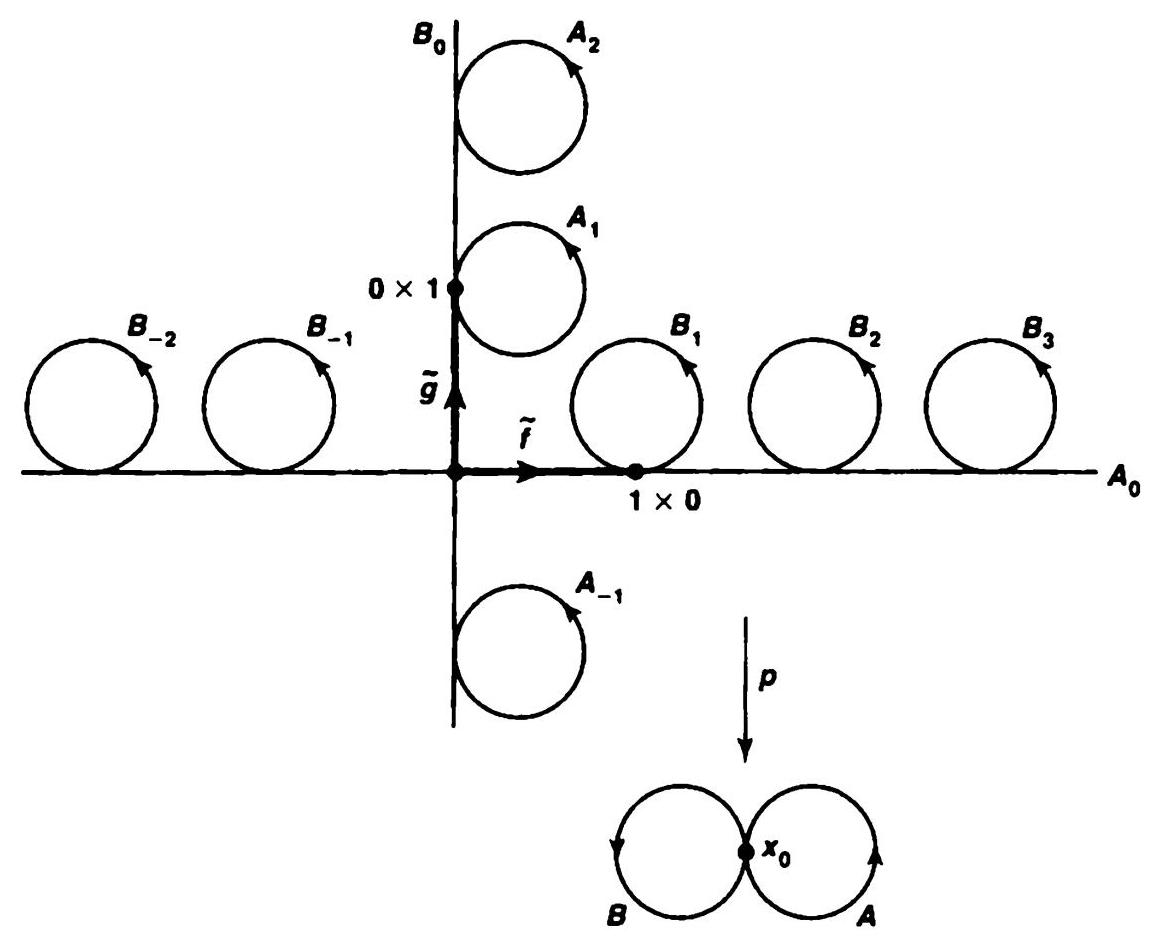
\includegraphics[width=1.0\textwidth]{images/60.1.jpg}
\end{center}
\hspace*{3em} 

Figure 60.1

To prove this assertion, let us lift each of these to a path in \(E\) beginning at the origin. The path \(f * g\) lifts to a path that goes along the \(x\) -axis from the origin to \(1 \times  0\) and then goes once around the circle tangent to the \(x\) -axis at \(1 \times  0\) . On the other hand, the path \(g * f\) lifts to a path in \(E\) that goes along the \(y\) -axis from the origin to \(0 \times  1\) , and then goes once around the circle tangent to the \(y\) -axis at \(0 \times  1\) . Since the lifted paths do not end at the same point, \(f * g\) and \(g * f\) cannot be path homotopic.

We shall prove later that the fundamental group of the figure eight is, in fact, the group that algebraists call the ``free group on two generators.''
\end{proof}
\section*{Theorem 60.6. The fundamental group of the double torus is not abelian.}

\begin{proof}
	The double torus \(T\# T\) is the surface obtained by taking two copies of the torus, deleting a small open disc from each of them, and pasting the remaining pieces together along their edges. We assert that the figure eight \(X\) is a retract of \(T\# T\) . This fact implies that inclusion \(j : X \rightarrow  T\# T\) induces a monomorphism \({j}_{ * }\) , so that \({\pi }_{1}( {T\# T,{x}_{0}})\) is not abelian.
One can write equations for the \index{retraction@Retraction}retraction \(r : T\# T \rightarrow  X\) , but it is simpler to indicate it in pictures, as we have done in Figure 60.2. Let \(Y\) be the union of two tori having a point in common. First one maps \(T\# T\) onto \(Y\) by a map that collapses the dotted curcle to a point but is otherwise one-to-one; it defines a homeomorphism \(h\) of the figure eight in \(T\# T\) with the figure eight in \(Y\) . Then one retracts \(Y\) onto its figure eight by mapping each cross-sectional circle to the point where it intersects the figure eight. Then one maps the figure eight in \(Y\) back onto the figure eight in \(T\# T\) by the map \({h}^{-1}\) .

\begin{center}
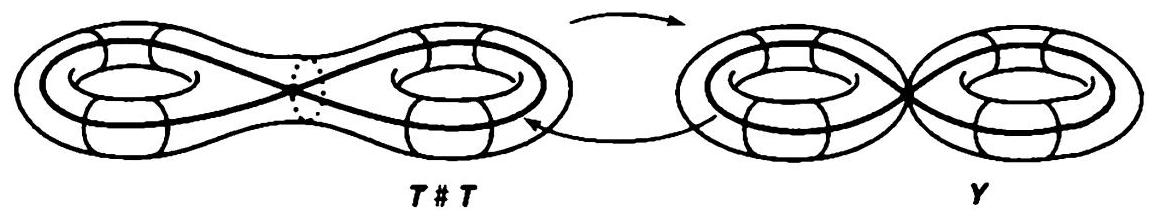
\includegraphics[width=1.0\textwidth]{images/60.2.jpg}
\end{center}
\hspace*{3em} 

Figure 60.2
\end{proof}
\begin{corollary}
	The 2-sphere, torus, projective plane, and double torus are topologically distinct.
\end{corollary}

\section*{Exercises}
\begin{enumerate}[itemsep=0.4em, parsep=0pt, topsep=0pt, partopsep=0pt, leftmargin=*, label=\arabic*., ref=\arabic*]
\item Compute the fundamental groups of the ``solid torus'' \({S}^{1} \times  {B}^{2}\) and the product space \({S}^{1} \times  {S}^{2}\) .
\item Let \(X\) be the quotient space obtained from \({B}^{2}\) by identifying each point \(x\) \index{Covering space!of \({S}^{1}\)}of \({S}^{1}\) with its \index{antipode@Antipode}antipode \(- x\) . Show that \(X\) is homeomorphic to the projective plane \({P}^{2}\) .
\item Let \(p : E \rightarrow  X\) be the map constructed in the proof of Lemma 60.5. Let \({E}^{\prime }\) be the subspace of \(E\) that is the union of the \(x\) -axis and the \(y\) -axis. Show that \(p \mid  {E}^{\prime }\) is not a covering map.
\item The space \({P}^{1}\) and the covering map \(p : {S}^{1} \rightarrow  {P}^{1}\) are familiar ones. What are they?
\item Consider the covering map indicated in Figure 60.3. Here, \(p\) wraps \({A}_{1}\) around \(A\) twice and wraps \({B}_{1}\) around \(B\) twice; \(p\) maps \({A}_{0}\) and \({B}_{0}\) homeomorphically onto \(A\) and \(B\) , respectively. Use this \index{Torus!covering space of}covering space to show that the fundamental group of the figure eight is not abelian. \begin{center} 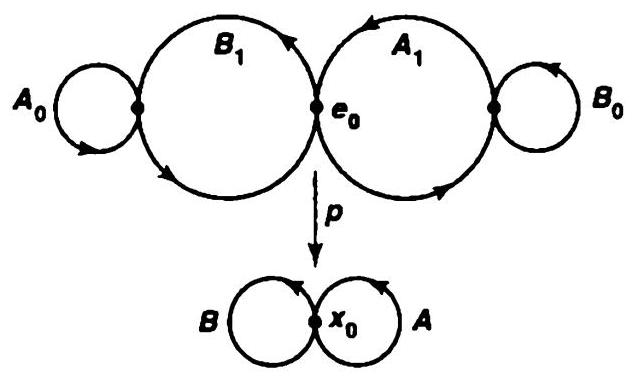
\includegraphics[width=0.5\textwidth]{images/60.3.jpg} \end{center} \hspace*{3em} Figure 60.3
\end{enumerate}